\documentclass[11pt,oneside]{book}
\usepackage{fontspec}
\usepackage{xeCJK}
\setmainfont{Latin Modern Roman}
\setCJKmainfont[ItalicFont={Noto Serif CJK JP},BoldItalicFont={Noto Serif CJK JP Bold}]{Noto Serif CJK JP}
\setCJKsansfont{Noto Sans CJK JP}
\setCJKmonofont{Noto Sans Mono CJK JP}
\newfontfamily\proseunicodefont{DejaVu Serif}
\usepackage[margin=1in]{geometry}
\usepackage{microtype}
\usepackage{amsmath,amssymb,amsthm,mathtools,bm}
\usepackage{graphicx}
\usepackage{xcolor}
\usepackage{booktabs}
\usepackage{array}
\usepackage{longtable}
\usepackage{enumitem}
\usepackage{float}
\usepackage{caption}
\usepackage{hyperref}
\usepackage{fancyhdr}
\usepackage{tikz}
\usetikzlibrary{arrows.meta,positioning,calc,decorations.pathmorphing}

\hypersetup{
  colorlinks=true,
  linkcolor=blue!50!black,
  urlcolor=blue!50!black,
  citecolor=blue!50!black
}

\setlength{\parskip}{0.5em}
\setlength{\parindent}{0pt}
\setlist[itemize]{topsep=0.25em,itemsep=0.2em}
\setlist[enumerate]{topsep=0.25em,itemsep=0.2em}
\setlength{\headheight}{40pt}
\numberwithin{equation}{chapter}

\newtheorem{theorem}{定理}[chapter]
\newtheorem{proposition}[theorem]{命題}
\newtheorem{lemma}[theorem]{補題}
\newtheorem{corollary}[theorem]{系}
\theoremstyle{definition}
\newtheorem{definition}[theorem]{定義}
\newtheorem{example}[theorem]{例}
\theoremstyle{remark}
\newtheorem{remark}[theorem]{注意}

\providecommand{\ket}[1]{\left\lvert#1\right\rangle}
\providecommand{\bra}[1]{\left\langle#1\right\rvert}
\providecommand{\braket}[2]{\left\langle#1\,\middle|\,#2\right\rangle}
\providecommand{\expect}[1]{\left\langle#1\right\rangle}
\newcommand{\lectureoverview}[1]{\paragraph{概観。} #1}
\newenvironment{classroomqa}{%
  \par\medskip
  \begin{minipage}{0.96\textwidth}
}{%
  \end{minipage}
  \par\medskip
}
\newcommand{\audiencequestion}[1]{\noindent\textbf{受講者からの質問。} #1\par\smallskip}
\newcommand{\lecturerresponse}[1]{\noindent\textbf{回答。} #1\par}
\newcommand{\lecturetimestamp}[1]{\footnote{講義時刻： #1.}}
\newcommand{\lectureframe}[1]{\par\smallskip{\centering\footnotesize\itshape 講義映像： #1.\par}}
\newcommand{\editorialnote}[1]{\footnote{編集上の補足： #1}}

\makeatletter
\newcommand{\course@headerfont}{\normalfont\small\itshape}
\newcommand{\course@pagefont}{\normalfont\small}
\newcommand{\course@headerraise}{14pt}
\newlength{\course@headerboxheight}
\setlength{\course@headerboxheight}{\dimexpr\headheight-\course@headerraise-9pt\relax}
\newcommand{\course@leftheadbox}[1]{%
  \raisebox{\course@headerraise}{%
    \parbox[t][\course@headerboxheight][t]{0.82\textwidth}{%
      \raggedright\course@headerfont\strut\MakeUppercase{#1}\strut%
    }%
  }%
}
\newcommand{\course@rightheadbox}[1]{%
  \raisebox{\course@headerraise}{%
    \parbox[t][\course@headerboxheight][t]{0.82\textwidth}{%
      \raggedleft\course@headerfont\strut\MakeUppercase{#1}\strut%
    }%
  }%
}
\renewcommand{\chaptermark}[1]{\markboth{\MakeUppercase{\chaptername\ \thechapter.\ #1}}{}}
\renewcommand{\sectionmark}[1]{\markright{\MakeUppercase{\thesection\hspace{0.4em}#1}}}
\fancyhf{}
\fancyhead[L]{\course@leftheadbox{\leftmark}}
\fancyhead[R]{\course@pagefont\thepage}
\renewcommand{\headrulewidth}{0.5pt}
\pagestyle{fancy}
\fancypagestyle{plain}{%
  \fancyhf{}
  \fancyhead[L]{\course@leftheadbox{\leftmark}}
  \fancyhead[R]{\course@pagefont\thepage}
  \renewcommand{\headrulewidth}{0.5pt}
}
\makeatother

\renewcommand{\contentsname}{目次}
\renewcommand{\chaptername}{章}
\renewcommand{\figurename}{図}
\renewcommand{\tablename}{表}
\renewcommand{\proofname}{証明}
\renewcommand{\bibname}{参考文献}
\emergencystretch=2em
\pdfstringdefDisableCommands{\def\proseunicodefont{}}

\hypersetup{
  pdftitle={Quantum Entanglement, Part 3},
  pdfauthor={Lectures by Leonard Susskind; companion edition by LazyingArt LLC},
  pdfsubject={Independently edited companion notes for the 2006 Fall lecture course},
  pdfcreator={LaTeX with hyperref}
}
\graphicspath{{../../../generated_course_notes/supplementary/quantum_entanglement/2006_fall_part_3/figures/}{../../../generated_course_notes/supplementary/quantum_entanglement/2006_fall_part_3/assets/}}
\begin{document}
\frontmatter
\hypersetup{pageanchor=false}
\begin{titlepage}
\thispagestyle{empty}
\begin{tikzpicture}[remember picture,overlay]
  \node[anchor=center,inner sep=0] at (current page.center) {%
    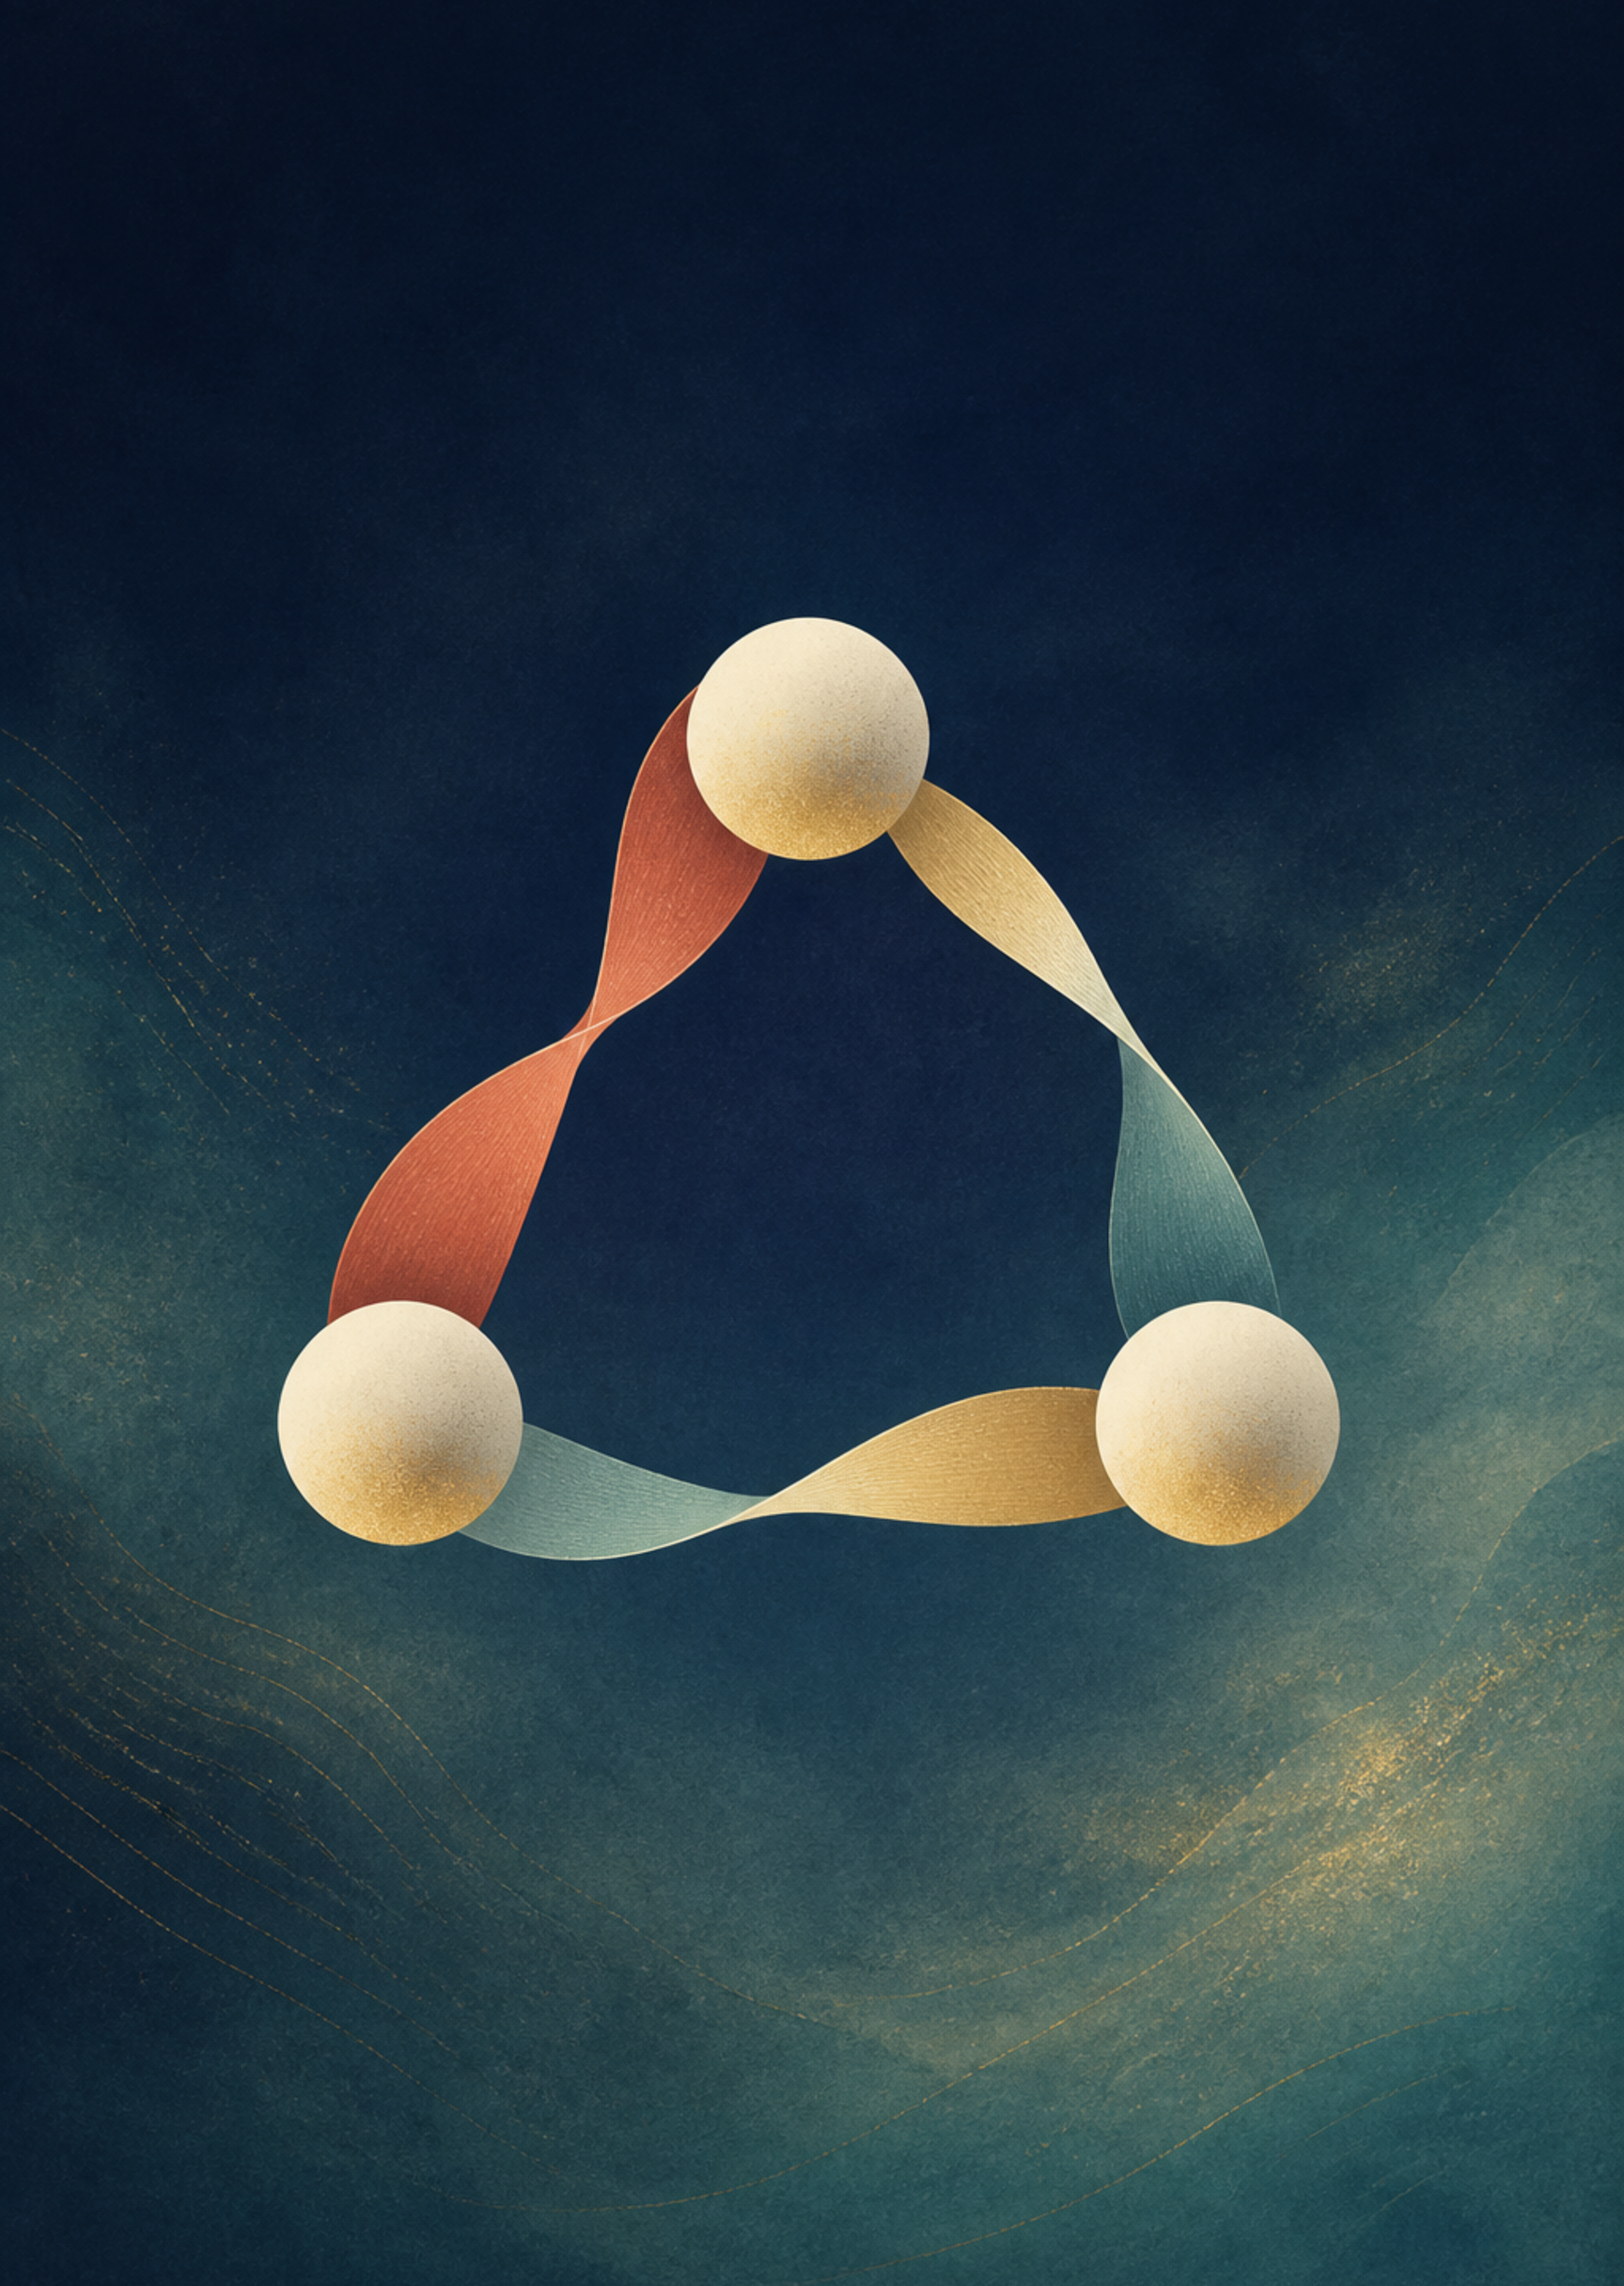
\includegraphics[height=\paperheight,keepaspectratio]{../../../generated_course_notes/supplementary/quantum_entanglement/2006_fall_part_3/assets/cover-art.png}%
  };
  \node[
    anchor=north west,
    align=left,
    text width=0.78\paperwidth,
    fill=white,
    fill opacity=0.9,
    rounded corners=8pt,
    inner xsep=10pt,
    inner ysep=8pt
  ] at ([xshift=0.08\paperwidth,yshift=-0.06\paperheight]current page.north west) {%
    {\fontsize{30}{33}\selectfont\bfseries\color{black!88} 量子もつれ 第3部\\[0.85em]}
    {\large\color{black!72} 日本語版 / 2006 fall part 3}
  };
  \node[
    anchor=south west,
    align=left,
    text width=0.68\paperwidth,
    fill=white,
    fill opacity=0.82,
    text opacity=1,
    rounded corners=6pt,
    inner sep=12pt
  ] at ([xshift=0.08\paperwidth,yshift=0.08\paperheight]current page.south west) {%
    {\normalsize\color{black!78} 原講義：Leonard Susskind\\[0.35em]}
    {\small\color{black!72} 講義補助版：\href{https://lazying.art}{LazyingArt LLC} / \href{https://github.com/lachlanchen/Video2Book}{Video2Book}}
  };
\end{tikzpicture}
\mbox{}
\end{titlepage}
\hypersetup{pageanchor=true}

\clearpage
\chapter*{本ノートについて}
本独立編集の補助ノートは、レナード・サスキンドによる量子もつれに関する2006年の講義コースの第3部を追うものである。これらは機械文字起こし、字幕、および選択された黒板画像から再構成され、その後、利用可能な原資料と照合された。これはサスキンド教授による原著ではなく、同教授による査読や承認を受けたものでもない。

本版は\href{https://lazying.art}{LazyingArt LLC}がオープンソースの\href{https://github.com/lachlanchen/Video2Book}{Video2Book}ツールキットを用いて作成した。機械文字起こしは別途利用可能であり、認識誤りを含む可能性がある。編集上の明確化および自明でない再構成は脚注で識別されている。
\clearpage
\tableofcontents
\mainmatter
\chapter{特殊相対性理論：基準系、同時性、ローレンツ変換}

相対性とは、物理法則がそれを記述するために用いる慣性系に依存しないという原理である。最初の課題は運動学である。すなわち、空間、時間、運動、同期の意味、および一つの慣性系から別の慣性系への変換である。力学はその後に来る。相対論的エネルギー、運動量、力、ニュートンの運動方程式の類似物、そして\(E=mc^2\)の意味である。その構造が確立すれば、一般相対性理論に概念的アプローチできる。曲がった時空、与えられた重力場中の粒子の運動、ブラックホール、宇宙の膨張を通じてであり、アインシュタインの場の方程式を解くという困難な問題から始めることなく。

概念的厳密さと数学的厳密さの区別は重要である。我々は故意に偽である近似を用いることはない。むしろ、重力場が時計、粒子、幾何学に何をするかに重点を置き、場の方程式の任意の解を構成するために必要な道具立ては後回しにする。特殊相対性理論はより明示的に扱わなければならない。その後の推論のすべてがその運動学に依拠しているからである。

したがって、出発すべき正しい場所は、有名な公式ではなく、観測者が場所と時間によって何を意味するかの正確な説明である。

\section{基準系とは物理的な座標系である}

空間が任意に細かい物差しの格子で満たされていると想像せよ。各格子点は三つの空間座標でラベル付けされ、各点には時計がある。棒と時計が一緒になって基準系を構成する。

\begin{definition}
\emph{事象}とは、一つの場所と一つの時間に起こるものである。一次元空間ではその座標は\((x,t)\)と書かれ、三次元では\((x,y,z,t)\)である。
\end{definition}

ニュートン物理学は強力な仮定を加える。すべての理想的な時計は一度で永久に同期できる。時間は普遍的である。時計は動かされてもよく、観測者は腕時計を持ち歩いてもよいが、誰もがどこでも同じ\(t\)に同意するとされる。これは絶対時間と呼ばれることがあり、神の時間、全世界のための一つの時計として思い描くことができる。

相対性原理はアインシュタインより古い。その自然な描像は、完全に滑らかなレールの上をあまりに一様に動くため何もガタガタ揺れない列車である。列車の中では、駅に停まっている列車でするのとまったく同じようにボールを投げて受け取ることができる。ジャグリングは驚くほど完全な小さな力学実験である。タイミング、重力、位置合わせ、軌道の繰り返し制御を必要とする。列車が一定速度で動くなら、それらの規則はどれも変わらない。真上に投げたボールは同じ手に戻る。列車がその下から滑り出ることはない。ガリレオはこの事実を認識し、ニュートンは運動法則において体系的に表現した。

ガリレオ以前には、動く列車はボールが空中にある間に進むはずであり、ジャグラーはそれを取り戻すために後ろや前へ手を伸ばさねばならないと推論する誘惑があった。誤りは、ボールが手を離れるときすでに列車の水平速度を共有していることを忘れることである。滑らかに動く車両内に限定された実験は、絶対的静止の特別な状態を明らかにしない。観測できるのは二つの列車の間の相対運動だけである。

したがって、静止した列車と一様に動く列車は二つの慣性系である。アインシュタイン以前には、それらはガリレイ変換によって関係づけられていた。

\section{時空を描く}

ここでは\(y\)と\(z\)を一時的に抑制し、時間を縦に、位置\(x\)を横に描く。図中の各点は事象である。線\(x=0\)は空間原点の履歴、すなわち\emph{世界線}である。隣接する縦線\(x=1,2,3,\ldots\)は他の格子点の世界線である。横線は共通の時間をもつ事象の集合である。

\begin{figure}[H]
\centering
\includegraphics[width=0.62\textwidth]{lecture_01_figure_02.png}
\caption{静止系の時間軸と空間格子の最初の世界線。}
\lectureframe{00:16:38}
\end{figure}

同じ構成は理想化された図ではより明確である：

\begin{figure}[H]
\centering
\begin{tikzpicture}[scale=0.95]
\draw[->] (-1.2,0) -- (5.2,0) node[right] {$x$};
\draw[->] (0,-0.2) -- (0,4.8) node[above] {$t$};
\foreach \x in {-1,1,2,3,4}
  \draw[gray!65] (\x,0) -- (\x,4.4);
\foreach \y in {1,2,3,4}
  \draw[gray!65] (-1.0,\y) -- (4.4,\y);
\fill (0,0) circle (1.5pt);
\node[below left] at (0,0) {$0$};
\node[left] at (0,1) {$1$};
\node[left] at (0,2) {$2$};
\node[left] at (0,3) {$3$};
\node[below] at (1,0) {$1$};
\node[below] at (2,0) {$2$};
\node[below] at (3,0) {$3$};
\end{tikzpicture}
\caption{静止した時空格子。縦線は一定の位置を、横線は一定の時間をもつ。}
\end{figure}

格子は想像上のものであり、その間隔は任意である。メートル、センチメートル、ミクロン、あるいは物理的に意味をなすさらに小さな間隔のいずれでもよい。その目的は、すべての事象に正確な座標を割り当てることである。

「基準系」という語は今や操作的な内容を持つ。それは単なる視点や、ある方向を見ている人ではない。それは拡張された座標装置である。事象が与えられれば、局所的な物差しがそれがどこで起こったかを指定し、局所的な時計がいつ起こったかを指定する。そうすれば他の物理量を系の間で比較できる。粒子の位置と速度、そのエネルギー、おそらく物体の温度、そして最終的にはその運動量と力である。最も単純な比較は\(x\)と\(t\)を含むものであるから、そこから始める。

次に、正の\(x\)方向に一定の速度\(v\)で運動する列車の上に第二の格子を置く。原点は\(t=0\)で一致するように選ぶ。運動する原点はそのとき次に従う。
\begin{equation}
x=vt.
\end{equation}
列車に固定された他のすべての点は、平行に傾いた世界線に従う。この傾きは、時間が経過するにつれて列車が位置を変えるという幾何学的な陳述にすぎない。

列車の後端の点がプライム付き原点であるとする。\(t=0\)においてそれは駅の原点と一致する。より後の時刻\(t\)において、その静止座標は\(vt\)である。したがって座標\(x\)にある近くの事象は、列車の原点からわずか\(x-vt\)しか離れていない。これが、この変換が恣意的な代数規則ではなく引き算である理由である。

\((x,t)\)を駅系における事象の座標、\((x',t')\)を列車系におけるその座標とする。ガリレオとニュートンは普遍時間を保持する。
\begin{equation}
t'=t.
\end{equation}
時間\(t\)の間に、運動する原点は\(vt\)だけ進むので、その原点から事象までの距離は
\begin{equation}
x'=x-vt.
\end{equation}
である。合わせると、
\begin{align}
t'&=t, & x'&=x-vt.
\label{eq:galilean-forward}
\end{align}
プライムなしの座標について解くと逆変換が得られる。
\begin{align}
t&=t', & x&=x'+vt'.
\label{eq:galilean-inverse}
\end{align}

\begin{figure}[H]
\centering
\includegraphics[width=0.72\textwidth]{lecture_01_figure_03.png}
\caption{二つの時空格子の隣に書かれたガリレイ変換。}
\lectureframe{00:21:57}
\end{figure}

最初の組は、運動する観測者に、静止した観測者から与えられた座標をどのように変換するかを教える。逆の組は逆に変換し戻す。記述間のこの相互的な変換が、ガリレイ相対性の数学的内容である。

逆の空間の式における置き換え\(t\to t'\)が無害であるのは、ガリレイ理論がすでに\(t=t'\)を宣言しているからにすぎない。この仮定に今気づいておくことは有用である。アインシュタインの理論では二つの時間座標が異なるものになり、そのような置き換えはもはや自動的にはできない。

\begin{classroomqa}
\audiencequestion{時計を持ち去ってから再び持ち帰ったとき、その運動が最初に時計を速め、次に遅くして、時計を比較するときに効果を隠したのではないと、どうして知ることができるだろうか。
\lecturetimestamp{00:23:09}}
\lecturerresponse{ガリレオは現代的な精度で普遍時間を確立できなかったであろう。それは物理的な推測であった。我々はその推測を多くの方法で検証できる。良い時計を反対方向に持ち運び、北--南の旅だけでなく東--西の旅も繰り返し、一方の時計を他方の周りで動かし、あるいは時計を一緒にすることなく時刻信号を交換する。通常の速度では、そのようなすべての検証は非常に高い精度で一致する。十分に正確な時計または十分に大きな速度では、小さな不一致が現れる。普遍時間のこの失敗は実験の欠陥ではなく、特殊相対性理論が説明しなければならない現象の一つである。}
\end{classroomqa}

\section{ガリレイ不変量とニュートンの法則}

不変量とは、議論しているすべての慣性観測者が一致する量である。座標それ自体は不変である必要はない。重要なのは、それらから組み立てられた法則が同じ形を保つかどうかである。

この語は名詞としても形容詞としても用いられる。数が不変量であり得るし、方程式が変換の下で不変であり得る。不変な量と不変な法則の区別は、よくある混乱を防ぐ。相対性理論は、すべての観測者がすべてについて同じ座標を得ると主張しているのではない。それは、彼らの測定を結びつける物理法則が同じ形を持つと主張しているのである。

位置\(x_1\)と\(x_2\)にある二つの同時事象を取る。式~\eqref{eq:galilean-forward}は次を与える。
\begin{align}
x_1'&=x_1-vt,\\
x_2'&=x_2-vt.
\end{align}
したがってそれらの隔たりは
\begin{equation}
x_2'-x_1'=(x_2-vt)-(x_1-vt)=x_2-x_1.
\end{equation}
である。ガリレイ物理学では、個々の位置は不変でなくても、同じ時刻に起こる事象間の距離は不変である。

\begin{classroomqa}
\audiencequestion{その引き算における\(t\)の二つの出現は本当に同じ時刻だろうか。
\lecturetimestamp{00:28:16}}
\lecturerresponse{はい。我々は二つの事象を意図的に\((x_1,t)\)と\((x_2,t)\)に選んだ。それらは一つの水平な等時刻線上にある。したがって共通項\(vt\)は相殺される。もし事象が異なる時刻に起こったなら、この議論は不変な空間的隔たりを確立しないであろう。}
\end{classroomqa}

次に、粒子を軌道\(x(t)\)によって記述する。列車の観測者は
\begin{equation}
x'(t)=x(t)-vt.
\end{equation}
を割り当てる。1回微分すると、おなじみの速度の加法則
\begin{equation}
\frac{dx'}{dt}=\frac{dx}{dt}-v.
\end{equation}
が得られる。位置と速度は座標系に依存する。矢のそばを移動する観測者は、線路のそばに立つ観測者よりも矢がゆっくり進むのを見る。

もう一度微分する。相対速度\(v\)は一定であるから、
\begin{equation}
\frac{d^2x'}{dt^2}=\frac{d^2x}{dt^2}.
\end{equation}
加速度はガリレイ変換の下で不変である。このことは、ニュートンの法則がなぜ位置や速度ではなく加速度を用いて書かれるのかを強く示唆している。

これは観測される物体の加速度であり、列車の観測者の加速度ではない。両方の座標系は慣性系であるから、どちらの座標系も他方に対して加速していない。物体はどちらの記述の中でも左または右に加速しうるし、2人の観測者は、物体の位置と速度については一致しないにもかかわらず、その加速度の値については一致する。

2つの粒子が互いに力を及ぼし合い、その力が同時的な隔たりのみに依存するとしよう。その隔たりは不変であるから、力も不変である。質量もまた本質的で座標系に依存しない性質であるならば、すべての慣性観測者は
\begin{equation}
F=ma
\end{equation}
をまったく同じ形で書くことができる。ニュートン力学はガリレイ変換の下で不変である。それは単にもっともらしいだけでなく、通常の速度の領域の全体にわたって極めて正確である。

この議論は、大きさが距離の関数であるような、ニュートン重力や静電場のようなおなじみの中心力に当てはまる。すべてのガリレイ観測者は共通の時刻におけるその距離について一致するので、力についても一致する。力と加速度が固定されれば、整合性は彼らが質量についても一致することを要求する。1キログラムの物体は、列車で運ばれても1キログラムの物体のままである。\(F=ma\)の中のすべての記号が同じ不変な構造に当てはまる。

\section{光はガリレイの規則に当てはまらない}

電磁気学が困難を生み出す。マクスウェル方程式は、空虚な空間を確定した速さ\(c\)で伝わる波を予言する。マクスウェル方程式が自然の法則であり、自然の法則がすべての慣性系で同じであるならば、すべての慣性観測者は同じ\(c\)を得なければならない。

ガリレイの運動学は別のことを予言する。静止系で右向きに進む光パルスは次を満たす。
\begin{equation}
x=ct.
\end{equation}
空間の変換を適用すると次が得られる。
\begin{equation}
x'=x-vt=(c-v)t.
\end{equation}
\(t'=t\)であるから、列車の観測者は速さ\(c-v\)を測定することになる。

矛盾は鋭く述べることができる。マクスウェル方程式がその形を保つならば、それらはプライム系で\(c\)を予言する。ガリレイ変換が保たれるならば、それは\(c-v\)を予言する。\(v\ne0\)であるとき、両方が厳密でありうることはない。

この結果は、光が媒質中の通常の波のように振る舞うならば、まったく自然に見える。水面波とともに動く船は、より低い相対波速度を測る。静止した空気中を動く聴者は、空気に対する聴者の運動だけずれた音速を測る。したがって19世紀の物理学者たちは、優先的な静止状態、すなわちマクスウェル方程式が最も単純な形をとり、光が\(c\)で進むエーテル系へと導かれた。そのような優先的な系に対する運動を検出するために設計された実験は、対応する効果を何も見いださなかった。

可能な実験配置はいくつかあったが、それらの共通の目的は、異なる運動状態または運動方向にある観測者について光の伝播を比較することであった。いずれも予想されたガリレイ的ずれを明らかにしなかった。この失敗は小さな技術的厄介事ではなかった。それは、相対性原理、マクスウェル方程式、そして受け継がれた空間と時間の概念の間の選択を迫った。

アインシュタインはこの対立にいっそう直接的に取り組んだ。若いころ彼は光波を追いかけることを想像した。もしそれに追いつくことができれば、その振動する電磁的パターンは空間に凍りついて静止するであろうが、マクスウェル方程式はそのような静止した光波を許さない。彼はマクスウェルの理論と相対性原理を基本的なものとして扱い、次にわれわれの座標に隠された仮定を再検討することを選んだ。

この再構成は2つの要請に基づいている。
\begin{enumerate}
\item 物理法則はすべての慣性系で同じ形をとる。
\item 真空中の光はすべての慣性系で同じ速さ\(c\)をもつ。
\end{enumerate}

第2の要請はガリレイ変換と共存できない。速度の加法則よりも深い何かが変わらなければならない。アインシュタインの経済的な選択は、2つの要請を保ち、一見無害なガリレイの式\(t'=t\)を再検討することである。

\section{遠方の時計の同期}

空間的な距離は棒で配置できるが、離れた時計には同期の規約が必要である。中点にいる観測者から等距離に二つの時計を置く。各端点の時計が定められた時刻を指したとき、その時計に閃光を発させるとする。二つの閃光が同時に中点へ届けば、端点の時計は同期していると呼ぶ。一方の閃光が先に届けば、対応する時計を調整し、手順を繰り返す。

\emph{中点}という語は、その座標系ですでに配置された棒を用いて定義される。したがってこの判定には二つの別個の要素が含まれる。端点からの空間的距離が等しいことと、信号の到着時刻が等しいことである。どちらの要素も落としてよいものではない。この手順を格子全体で繰り返すことで、ニュートンが単に仮定していた水平な等時線が与えられる。

この定義が光を用いるのは、公準がすべての慣性系で光に同じ速さを割り当てているからである。すべての隣接する対についてこのように扱えば、格子全体が同期した時計の族を備えることになる。

次に、第二の格子を第一の格子に対して運動させる。運動する装置の中点は、それ自身の座標系では二つの運動する端点の中間に留まる。しかし静止した装置に対しては、一方の到来する閃光へ向かい、他方から遠ざかる。静止した時計に従って同時に発せられた閃光は、運動する中点に同時には届かない。運動する観測者は同じ中点と光の規則を適用するので、その観測者はそれらの発光を同時とは呼べない。各座標系は自身の時計を首尾一貫して同期させるが、二つの同期は一致しない。

これは光の有限な伝播時間によって生じる目の錯覚ではない。各観測者は光が届くのに時間がかかることを知っており、同じ速さ\(c\)を用いてそれを補正する。それでも不一致は残る。なぜなら観測者たちは同じ遠方の事象の対を同時なものとして選ばないからである。同時性の見かけだけでなく、同時性そのものが相対的である。

\begin{classroomqa}
\audiencequestion{光ではなく音で時計を同期させれば、この結論を避けられるだろうか。
\lecturetimestamp{00:49:03}}
\lecturerresponse{音は空気が静止している座標系では同期信号として機能するが、その測定される速さはすべての慣性系で同じではない。静止した空気の中を進む開放的な列車は、音を伝える媒質に対して運動しているので、そこでは前方と後方の音信号は対称には振る舞わない。光は公準によって異なる。すなわち、その静止系が一人の観測者を選び出すような検出可能な光の媒質は存在しない。したがって我々は光を用い、その帰結を追う。}
\end{classroomqa}

定性的な不一致は明らかである。次に、運動する観測者がどの事象を同時と呼ぶかを正確に計算する。

\section{光線による作図}

作図には、次の単位を選ぶと便利である。
\begin{equation}
c=1.
\end{equation}
このとき距離の一単位は、光が時間の一単位で進む距離である。すなわち光秒と秒、あるいは光年と年を組にする。空間と時間は同じ単位を持ち、速度は無次元となり、光線は\(45^\circ\)に現れる。右向きの光線は
\begin{equation}
x=t+d,
\end{equation}
であり、左向きの光線は
\begin{equation}
x=-t+d'.
\end{equation}
である。原点を通る二つの光線は単に\(x=t\)と\(x=-t\)である。光より遅い物体に属する時間的軌道は、垂直軸に近い側にある。仮想的な超光速の軌道は、水平軸に近い側にある。

図中の角度は、この単位の選択によって初めて意味を持つ。メートルと秒では、光線は一秒間にほぼ\(3\times10^8\)メートルを進むので、ほとんど水平に見えるであろう。距離に光秒を選ぶと水平軸が再スケールされ、因果的な幾何学が見えるようになる。

運動する格子の中の三本の平行な世界線を考える。
\begin{equation}
x=vt,\qquad x=vt+L,\qquad x=vt+2L.
\label{eq:moving-worldlines}
\end{equation}
中央の世界線は、二つの外側の点の間で同時性を判定する観測者に属する。三つの点はすべて一様に運動し、プライム付きの座標系でそれらの相対的な配置を保つ。

\begin{figure}[H]
\centering
\includegraphics[width=0.72\textwidth]{lecture_01_figure_04.png}
\caption{前方の光線\(x=t\)が中央の運動する世界線と出会う。}
\lectureframe{01:02:33}
\end{figure}

完全な幾何学は、黒板の前に立つ人の妨げなしに描くことができる。

\begin{figure}[H]
\centering
\begin{tikzpicture}[scale=0.95]
\draw[->] (-0.5,0) -- (6.5,0) node[right] {$x$};
\draw[->] (0,-0.2) -- (0,4.3) node[above] {$t$};
\draw[blue] (0,0) -- (1.4,4.0);
\draw[blue] (2.0,0) -- (3.4,4.0);
\draw[blue] (4.0,0) -- (5.4,4.0);
\draw[red] (0,0) -- (3.08,3.08);
\draw[red] (3.08,3.08) -- (4.56,1.60);
\draw[red,dashed] (2.0,0) -- (4.56,1.60);
\fill (0,0) circle (1.5pt);
\fill (2.0,0) circle (1.5pt);
\fill (4.0,0) circle (1.5pt);
\fill (3.08,3.08) circle (1.5pt);
\fill (4.56,1.60) circle (1.5pt);
\node[left] at (0.55,1.55) {$x=vt$};
\node[left] at (2.45,1.9) {$x=vt+L$};
\node[right] at (4.72,1.9) {$x=vt+2L$};
\node[left] at (1.88,2.28) {$x=t$};
\node[above right] at (3.08,3.08) {$A$};
\end{tikzpicture}
\caption{光信号が運動する座標系の同時線を決定する。}
\end{figure}

原点から右向きの光線を送る。\(A\)を、それが中央の世界線と交わる点とする。\(A\)における二つの方程式は
\begin{align}
x&=t,\\
x&=vt+L.
\end{align}
である。代入すると
\begin{equation}
t=vt+L,
\end{equation}
となり、したがって
\begin{equation}
t_A=x_A=\frac{L}{1-v}.
\label{eq:point-a}
\end{equation}

\(A\)から、左向きに進む光線を右端の運動する世界線までさかのぼる。その方程式は次の形をとる。
\begin{equation}
x+t=b.
\end{equation}
\(A\)を通るので、式~\eqref{eq:point-a}が定数を定める。
\begin{equation}
b=x_A+t_A=\frac{2L}{1-v}.
\end{equation}
したがって後ろ向きの光線は次を満たす。
\begin{equation}
x+t=\frac{2L}{1-v}.
\label{eq:backward-ray}
\end{equation}

右端の世界線との交点は次から従う。
\begin{align}
x+t&=\frac{2L}{1-v},\\
x&=vt+2L.
\end{align}
\(x\)を消去すると、
\begin{align}
(1+v)t
  &=2L\left(\frac{1}{1-v}-1\right)\\
  &=\frac{2Lv}{1-v},
\end{align}
よって
\begin{equation}
t=\frac{2Lv}{1-v^2}.
\end{equation}
\(x=vt+2L\)に代入すると次が得られる。
\begin{equation}
x=\frac{2L}{1-v^2}.
\end{equation}
座標そのものよりもそれらの比の方が重要である。
\begin{equation}
\frac{t}{x}=v.
\end{equation}
したがって、運動する時計によれば原点と同時であるすべての事象は次上にあり、
\begin{equation}
t=vx,
\label{eq:simultaneity-c-one}
\end{equation}
一方、運動する原点は次に従う。
\begin{equation}
x=vt.
\label{eq:moving-time-axis}
\end{equation}
二つの軸は\(45^\circ\)の光線のまわりに対称的に傾いている。

\(x=vt\)上のすべての点は同じプライム付き位置\(x'=0\)をもち、一方それらのプライム付き時間は変化する。\(t=vx\)上のすべての点は同じプライム付き時間\(t'=0\)をもち、一方それらのプライム付き位置は変化する。したがって一方の線はプライム付き時間軸であり、他方はプライム付き空間軸である。長い信号の構成は二番目の線を決定するために必要であった。それは運動する世界線だけから推論することはできなかった。

式~\eqref{eq:simultaneity-c-one}で通常の単位を復元するには次が必要である。
\begin{equation}
t=\frac{v}{c^2}x.
\label{eq:simultaneity-dimensional}
\end{equation}
因子\(c^2\)は、ニュートン的な描像が日常生活で非常によく成り立つ理由を説明する。\(c\)に比べて極めて小さい速度では、運動する同時線の傾きはきわめて小さい。

\begin{figure}[H]
\centering
\includegraphics[width=0.72\textwidth]{lecture_01_figure_05.png}
\caption{\(c=1\)のもとで、プライム付き時間軸と同時軸は光線に関して対称である。}
\lectureframe{01:15:40}
\end{figure}

\begin{figure}[H]
\centering
\begin{tikzpicture}[scale=1.0]
\draw[->] (-2.2,0) -- (5.2,0) node[right] {$x$};
\draw[->] (0,-0.2) -- (0,4.9) node[above] {$t$};
\draw[red] (0,0) -- (3.9,3.9);
\draw[red] (0,0) -- (-1.8,1.8);
\draw[blue] (0,0) -- (1.8,4.5);
\draw[blue,dashed] (0,0) -- (4.5,1.8);
\node[right] at (3.9,3.9) {$x=t$};
\node[left] at (-1.8,1.8) {$x=-t$};
\node[above] at (1.8,4.5) {$x'=0$};
\node[right] at (4.5,1.8) {$t'=0$};
\end{tikzpicture}
\caption{\(c=1\)単位でのプライム付き軸と不変な光線。}
\end{figure}

\section{ローレンツ変換の導出}

幾何学は各プライム付き座標がどこで消えるかを定める。運動する時間軸\(x=vt\)に沿って、\(x'=0\)でなければならない。運動する同時軸\(t=vx\)に沿って、\(t'=0\)でなければならない。それらの零点集合をもつ最も一般的な線形関係は次のように書ける。
\begin{align}
x'&=\frac{x-vt}{F(v)},\\
t'&=\frac{t-vx}{G(v)}.
\label{eq:fg-ansatz}
\end{align}
因子\(F\)と\(G\)は、軸がすでに位置づけられていても、プライム付き座標の目盛りがガリレイ的な目盛りと異なることを許す。線形性は空間と時間の一様性から従う。実験を平行移動しても変換則は変わらないからである。\editorialnote{この短い線形性の議論は、黒板での導出で暗黙に用いられていた仮定を明示する。}

この段階で、幾何学は多くを教えてくれたが、すべてではない。分子は軸の傾きを定める。それらはそれらの軸に沿った単位間隔を定めない。その残りの目盛り情報こそが、まさに\(F(v)\)と\(G(v)\)が表すものである。

ここで光速度の不変性を課す。\(x=t\)に従う右向きの光線はまた\(x'=t'\)にも従わなければならない。その光線に沿って、
\begin{align}
x'&=\frac{(1-v)t}{F(v)},\\
t'&=\frac{(1-v)t}{G(v)}.
\end{align}
光線上のすべての点に対する等号は次を要求する。
\begin{equation}
F(v)=G(v).
\end{equation}
したがって次のように書いてよい。
\begin{align}
x'&=\frac{x-vt}{F(v)},\\
t'&=\frac{t-vx}{F(v)}.
\label{eq:common-f}
\end{align}

この段階は、この代数において最初の真にアインシュタイン的な要請を用いる。同じ幾何学的な線が両方の観測者にとって光線であるので、\(c=1\)のとき、二つのプライム付き座標はそれに沿って等しく増加しなければならない。二つの方程式で因子が異なれば、プライム付き速度は1と異なることになる。

未知の関数が一つ残る。式~\eqref{eq:common-f}に\(F(v)\)を掛けると、
\begin{align}
F(v)x'&=x-vt,\\
F(v)t'&=t-vx.
\end{align}
第二の方程式に\(v\)を掛けて第一の方程式に加えると\(t\)が消去され、次が得られる。
\begin{equation}
(1-v^2)x=F(v)(x'+vt').
\end{equation}
同様に、
\begin{equation}
(1-v^2)t=F(v)(t'+vx').
\end{equation}
したがって逆変換は次である。
\begin{align}
x&=\frac{F(v)}{1-v^2}(x'+vt'),\\
t&=\frac{F(v)}{1-v^2}(t'+vx').
\end{align}

相対性原理は二つの系を相互的にする。駅が列車の動きを\(+v\)で見るなら、列車は駅の動きを\(-v\)で見る。したがって逆方程式は、\(v\)の符号を反転させた、順方向の方程式と同じ形をもたなければならない。それらの前因子は次を満たさなければならない。
\begin{equation}
\frac{F(v)}{1-v^2}=\frac{1}{F(v)}.
\end{equation}
ゆえに
\begin{equation}
F(v)^2=1-v^2,
\end{equation}
であり、\(v=0\)における恒等変換との連続性が正の根を選ぶ。
\begin{equation}
F(v)=\sqrt{1-v^2}.
\end{equation}

特定の光パルスに何も合わせていない。結果は、同期によって定まる軸、光の共通速度、およびどちらの慣性系も他方より特権的でないという要請から従う。

\(c=1\)とする単位でのローレンツ変換は次である。
\begin{align}
x'&=\frac{x-vt}{\sqrt{1-v^2}},\\
t'&=\frac{t-vx}{\sqrt{1-v^2}}.
\label{eq:lorentz-c-one}
\end{align}
その逆変換は次である。
\begin{align}
x&=\frac{x'+vt'}{\sqrt{1-v^2}},\\
t&=\frac{t'+vx'}{\sqrt{1-v^2}}.
\end{align}

\begin{figure}[H]
\centering
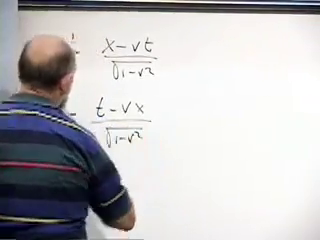
\includegraphics[width=0.76\textwidth]{lecture_01_figure_06.png}
\caption{黒板上で完成した\(c=1\)ローレンツ変換。}
\lectureframe{01:32:38}
\end{figure}

本質的な新しさはすでに時間の方程式に見えている。時間は単にある系から別の系へ変わらずに運ばれるのではない。プライム付き時間座標はプライムなしの時間と位置を混ぜ合わせる。したがって\(t=\text{constant}\)と\(t'=\text{constant}\)は異なる事象の集合を記述する。

混合項は、後から付け足される任意の補正ではない。これがなければ、直線 \(t'=0\) は水平のままであり、遠方の同時性は普遍的なものにとどまり、変換は光速を保つことができない。

\section{光速の回復と結果の確認}

\(c\ne1\) のとき、次元の整合性によって欠けていた因子が回復される。比 \(v^2/c^2\) は無次元であり、一方 \((v/c^2)x\) は時間の次元をもつ。したがって
\begin{align}
x'&=\frac{x-vt}{\sqrt{1-v^2/c^2}},\\
t'&=\frac{t-(v/c^2)x}{\sqrt{1-v^2/c^2}}.
\label{eq:lorentz-dimensional}
\end{align}
逆変換は \(v\) の符号を反転させることで得られる：
\begin{align}
x&=\frac{x'+vt'}{\sqrt{1-v^2/c^2}},\\
t&=\frac{t'+(v/c^2)x'}{\sqrt{1-v^2/c^2}}.
\end{align}

\begin{equation}
\gamma=\frac{1}{\sqrt{1-v^2/c^2}}
\end{equation}
を導入すれば、これらはおなじみの簡潔な形になるが、分母の形にしておくことで導出が見えるままになる。

数値的には \(c\simeq3\times10^8\,\mathrm{m/s}\) であるから、\(c^2\simeq9\times10^{16}\,\mathrm{m^2/s^2}\) となる。この大きな分母のため、同時性の傾きも因子 \(v^2/c^2\) も、ほとんどの力学実験では感知できない。それらが小さいことがガリレオの成功を説明するのであって、絶対時間が回復されるわけではない。

\begin{figure}[H]
\centering
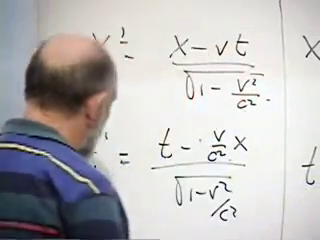
\includegraphics[width=0.76\textwidth]{lecture_01_figure_07.png}
\caption{\(c\) の因子を回復した後のローレンツ変換。}
\lectureframe{01:35:58}
\end{figure}

ただちに二つの確認ができる。まず \(v\ll c\) ととる。すると \(v^2/c^2\) は無視でき、通常の距離に対しては同時性の相対性の項 \(vx/c^2\) もまた無視できる。式~\eqref{eq:lorentz-dimensional}は
\begin{equation}
t'\approx t,\qquad x'\approx x-vt.
\end{equation}
に帰着する。ガリレイ相対性は低速近似として回復される。

第二に、光線を試す。\(c\) を回復すれば、右向きの光線は \(x=ct\) に従い、\(x=t\) ではない。代入すると
\begin{align}
x'&=\frac{(c-v)t}{\sqrt{1-v^2/c^2}},\\
t'&=\frac{(1-v/c)t}{\sqrt{1-v^2/c^2}}.
\end{align}
\(c-v=c(1-v/c)\) であるから、
\begin{equation}
x'=ct'.
\end{equation}
ダッシュ付きの観測者は同じ速さ \(c\) を測る。左向きの光線については、\(x=-ct\) を代入すれば同様に
\begin{equation}
x'=-ct'.
\end{equation}
が得られる。この変換はどちらの向きに進む光も正しく扱う。

\(x=t\) と \(x=ct\) の区別は、示唆に富む次元の確認である。前者は \(c=1\) となる単位系でのみ正しい。変換において通常の単位を回復しながら光線の方程式を自然単位のままにしておくと、二つの規約が混ざり、誤った結果を生む。次元の整合性はその誤りをただちに捉える。

\section{中点の判定基準}

\begin{classroomqa}
\audiencequestion{ある観測者が二つの閃光を同じ瞬間に受け取ったが、それらの光源の中間点にはいないとする。その観測者は、閃光が同時に発せられたと結論してよいだろうか。
\lecturetimestamp{01:42:55}}
\lecturerresponse{否。到着時刻が等しいことが発光時刻が等しいことを意味するのは、関連する座標系において二つの光源の空間的な中点にいる観測者だけである。一方の光源に近い受信者は、遠い方の閃光がより早く発せられていても、両方の閃光を一緒に受け取ることができる。運動する構成では、したがって中点の世界線 \(x=vt+L\) が本質的である。前方への光線 \(x=t\) をそれがその中点に出会うまで追い、次に後方への光線を \(x=vt+2L\) までたどる。その第二の端点の事象が、他の任意の等到着事象ではなく、運動する座標系によれば原点と同時である。}
\end{classroomqa}

われわれは完全な座標変換に到達したが、まだその最もよく知られた帰結には至っていない。次に続くのは長さの収縮、時間の遅れ、固有時間であり、さらに相対論的運動量とエネルギーが続く。基礎はすでに据えられている。各慣性系が同じ法則を用い、同じ光速を測ることができるのは、空間と時間が混ざり合い、遠方の同時性が世界に絶対的に属するのではなく座標系に属するからにほかならない。
\chapter{マクスウェル方程式、共変性、電磁波}

\lectureoverview{電場と磁場はローレンツ力を通じて荷電物質に作用するが、物質もまた場を生成し再配置しなければならない。本講義では、電磁気学のこの相互的な半分を定式化し、マクスウェル方程式がローレンツ共変であることを示し、その波動解を導出し、その後、局所的な保存を明白にする形で電荷と電流を復元する。講義全体を通じて\(c=1\)とする単位系を用いる。}

\section{電磁気学のもう半分}

すでに手元にある部分から始めよう。電荷\(q\)の粒子が速度\(\mathbf v\)で電場と磁場の中を運動するとき、力は
\begin{equation}
\mathbf F=q\bigl(\mathbf E+\mathbf v\times\mathbf B\bigr).
\label{eq:lorentz-force-three}
\end{equation}
である。因子\(q\)は不可欠である。荷電していない粒子は電磁気力を感じない。電場は粒子が瞬間的に静止しているときでも寄与するが、磁場の寄与はその運動に依存する。

式~\eqref{eq:lorentz-force-three}は、与えられた場が物質に何をするかを教える。しかし、何が場を決定するかは教えない。一方の物体の周りに電場を、他方の周りに磁場を、あるいは真空中を伝わる波を、何が生み出すのか。これらの問いに答える方程式がマクスウェル方程式である。

\begin{figure}[H]
\centering
\includegraphics[width=0.62\textwidth]{lecture_58_figure_02.png}
\caption{三ベクトルのローレンツ力とそのテンソル再定式化の始まり。}
\lectureframe{00:05:49}
\end{figure}

力の法則の相対論的形式は、我々が必要とする記法を先取りしている：
\begin{equation}
f^\mu=qF^\mu{}_{\nu}u^\nu.
\label{eq:lorentz-force-four}
\end{equation}
ここで\(u^\nu\)は四元速度、\(f^\mu\)は四元力、\(F^{\mu\nu}\)は\(\mathbf E\)と\(\mathbf B\)から組み立てられた反対称テンソルである。黒板にはまずこの表式の図式的な始まりのみが示される。\(u^\nu\)との縮約が、一つの自由な力の添字を残すために必要な欠けているベクトルを与える。

物質が場に反作用しなければならない物理的な理由がある。電磁波は電荷に当たり、それを加速し、エネルギーをそれに移すことができる。もし場が電荷に影響を与え得るのに、電荷が決して場に影響を与え得ないならば、そのエネルギーが引き出される場所が存在しないことになる。作用と反作用だけが議論のすべてではないが、エネルギー保存則はこの相互結合を不可避にする。

\section{変化する源が擾乱を送り出す}

点電荷はその位置から外向きまたは内向きの電場を生み出す。導線中の電流--荷電粒子の流れ--は、導線の周りを循環する磁場を生み出す。これらのよく知られた静的な描像はすでに二つの異なる幾何学的パターンを示している。電束は電荷から発散し、磁力線は電流の周りを巻く。

次に点電荷を突然動かす。その新しい位置の近くでは電場が再配置を始めなければならないが、遠方の観測者はその運動を即座に知ることはできない。信号が到着する時間ができるまで、古い場は遠方に残る。近傍領域と遠方領域の間には、場が変化している移動する前線が存在する。この移動する再配置が電磁的擾乱である。

電荷を前後に駆動すると、 successive な再配置が次々に続き、電磁波を形成する。これがアンテナの初等的な機能である。振動する電流が場の擾乱を外向きに送り出す。導線中の電流を反転させると、同じ議論の磁気版が得られる。\(\mathbf B\)の循環は反転しなければならないが、その反転は至る所に同時に現れるのではなく伝播する。

この因果的な描像はマクスウェル方程式に二つの目標を課す。それらは電荷と電流がどのように場を源として生み出すかを記述しなければならず、それらの場の変化が光より速く伝播しないことを許さなければならない。第二の目標は相対性の試金石でもある。もしマクスウェル方程式がすべての慣性系で同じ形を持ち、確定した波の速さを意味するならば、すべての慣性系がそれらから同じ速さを推論しなければならない。

\section{相対論的波動方程式の再検討}

ベクトル場に移る前に、スカラー場\(\phi(\mathbf x,t)\)、すなわち各時空点に一つの数を考える。一階微分の方程式
\begin{equation}
\partial_\mu\phi=0
\end{equation}
は、すべての時空微分が消えることを意味するであろう。場は定数となり、したがって波を運ぶことができない。非自明な相対論的波動方程式は二階微分を用いる：
\begin{equation}
\partial_\mu\partial^\mu\phi=0.
\end{equation}
ここで用いる符号規約では、
\begin{equation}
\left(\partial_t^2-\partial_x^2-\partial_y^2-\partial_z^2\right)\phi=0,
\label{eq:scalar-wave-four}
\end{equation}
あるいはより簡潔に、
\begin{equation}
\left(\partial_t^2-\nabla^2\right)\phi=0.
\end{equation}
である。\(c=1\)という選択により、時間と距離が両立する単位を持つ。通常の単位を復元すれば、\(1/c^2\)が二階時間微分の隣に置かれるであろう。

\(z\)軸に沿って伝わる波に対しては、場は\(z\)と\(t\)に依存し、\(x\)や\(y\)には依存しない。式~\eqref{eq:scalar-wave-four}は
\begin{equation}
\left(\partial_t^2-\partial_z^2\right)\phi=0.
\label{eq:scalar-wave-one}
\end{equation}
に帰着する。

\begin{figure}[H]
\centering
\includegraphics[width=0.56\textwidth]{lecture_58_figure_04.png}
\caption{電磁波のモデルとして用いられる一次元スカラー波動方程式。}
\lectureframe{00:47:03}
\end{figure}

その一般的な進行波の形は
\begin{equation}
\phi(z,t)=f(z-t)+g(z+t).
\end{equation}
である。プロファイル\(f(z-t)\)は\(z\)の増加する向きに進む。なぜなら、位相が固定された点は\(z-t=\text{constant}\)を満たすからである。プロファイル\(g(z+t)\)は反対向きに進む。どちらのプロファイルも正弦的である必要はなく、十分になめらかな任意の形状は形を変えずに平行移動する。

それでも正弦波は便利である：
\begin{equation}
\phi(z,t)=A\cos\!\bigl(k(z-t)\bigr).
\end{equation}
波数\(k\)は波長を決め、
\begin{equation}
\lambda=\frac{2\pi}{k}.
\end{equation}
\(k\)が大きいと空間的振動が速く波長が短くなり、\(k\)が小さいと波長が長くなる。これらの同じプロファイルはまもなく\(\mathbf E\)と\(\mathbf B\)の成分となる。

\section{マクスウェルに必要なベクトル解析}

マクスウェル方程式は内積、外積、発散、回転を用いて書かれる。後の成分計算ではまさにこれらのパターンを用いるので、ここで記法を一度立て直しておく価値がある。

通常の三次元ベクトル\(\mathbf a\)と\(\mathbf b\)に対し、内積はスカラー
\begin{equation}
\mathbf a\cdot\mathbf b
=a_xb_x+a_yb_y+a_zb_z.
\end{equation}
である。外積は別のベクトルであり、
\begin{align}
(\mathbf a\times\mathbf b)_x&=a_yb_z-a_zb_y,\\
(\mathbf a\times\mathbf b)_y&=a_zb_x-a_xb_z,\\
(\mathbf a\times\mathbf b)_z&=a_xb_y-a_yb_x.
\end{align}
残りの成分は巡回順序\(x\to y\to z\to x\)から従う。

微分演算子
\begin{equation}
\boldsymbol\nabla=
\left(\partial_x,\partial_y,\partial_z\right).
\end{equation}
を導入する。その成分は通常の数ではなく演算子であるが、内積と外積のパターンはなお用いることができる。ベクトル場\(\mathbf A\)に対し、
\begin{equation}
\boldsymbol\nabla\cdot\mathbf A
=\partial_xA_x+\partial_yA_y+\partial_zA_z
\label{eq:divergence}
\end{equation}
は発散であり、一方
\begin{align}
(\boldsymbol\nabla\times\mathbf A)_x
 &=\partial_yA_z-\partial_zA_y,\\
(\boldsymbol\nabla\times\mathbf A)_y
 &=\partial_zA_x-\partial_xA_z,\\
(\boldsymbol\nabla\times\mathbf A)_z
 &=\partial_xA_y-\partial_yA_x
\label{eq:curl}
\end{align}
は回転の成分である。

幾何学は式と同じくらい重要である。ベクトル場は、源から外へ流れ出るように見えるところで正の発散をもつ。循環するところで回転をもつ。点電荷の動径方向の電場は発散を例示し、電流を運ぶ導線の周りを巻く磁場は回転を例示する。空間的に一定のベクトル場はどちらももたない。

\section{真空中のマクスウェル方程式}

電荷と電流が存在しないとき、マクスウェル方程式は
\begin{align}
\boldsymbol\nabla\times\mathbf E&=-\partial_t\mathbf B,
\label{eq:faraday-vac}\\
\boldsymbol\nabla\cdot\mathbf B&=0,
\label{eq:gauss-b-vac}\\
\boldsymbol\nabla\times\mathbf B&=\partial_t\mathbf E,
\label{eq:ampere-vac}\\
\boldsymbol\nabla\cdot\mathbf E&=0.
\label{eq:gauss-e-vac}
\end{align}
である。二つの回転の方程式は\(\mathbf E\)と\(\mathbf B\)をほとんど交換するが、本質的な負符号がそれらを区別する。二つの発散の方程式は、考察している真空領域においてどちらの場も源をもたないことを述べている。電荷の源を復活させた後でも磁場の発散はゼロのままであり、通常の電磁気学には磁荷が含まれない。

\begin{figure}[H]
\centering
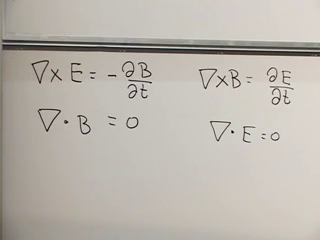
\includegraphics[width=0.76\textwidth]{lecture_58_figure_06.png}
\caption{四つの真空マクスウェル方程式。電場と磁場のほぼ対称性を示すように配置されている。}
\lectureframe{00:27:30}
\end{figure}

電荷密度\(\rho\)は最終的に式~\eqref{eq:gauss-e-vac}の右辺のゼロを置き換え、電流密度\(\mathbf J\)は式~\eqref{eq:ampere-vac}に入る。これらの項は一時的に延期する。源のない方程式は、変換構造と波動の仕組みを最も少ない雑多な要素で明らかにする。

それらはまたアインシュタインの難問を際立たせる。波を追いかけるガリレイ的観測者は、速度を差し引いてより小さな波の速さを測ることを期待するであろう。しかし、同じマクスウェル方程式がすべての慣性系で成り立つなら、各観測者は同じ単位波の速さを導く。打開策は、枠ごとに波動方程式を変えることではない。ローレンツ変換を用い、変換則がすでに知られている対象の中にマクスウェル方程式を示すことである。

\section{電場と磁場を一つのテンソルとして}

電場と磁場は反対称場テンソル
\begin{equation}
F^{\mu\nu}=
\begin{pmatrix}
0   & -E_x & -E_y & -E_z\\
E_x & 0    & -B_z & B_y\\
E_y & B_z  & 0    & -B_x\\
E_z & -B_y & B_x  & 0
\end{pmatrix},
\label{eq:l0203-field-tensor}
\end{equation}
に結合する。ここで行と列の順序は\(t,x,y,z\)である。反対称性
\begin{equation}
F^{\mu\nu}=-F^{\nu\mu},
\end{equation}
は対角成分をゼロにし、行列の下半分を上半分から決定する。時間-空間成分は\(\mathbf E\)を含み、純粋に空間的な成分は\(\mathbf B\)を含む。

\begin{figure}[H]
\centering
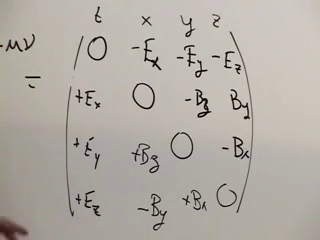
\includegraphics[width=0.58\textwidth]{lecture_58_figure_03.png}
\caption{完成した電磁場テンソル。その電場成分と磁場成分を含む。}
\lectureframe{00:32:05}
\end{figure}

\(F^{\mu\nu}\)の重要性は、六つの場の成分が一つの行列に収まることだけではない。ローレンツ変換の下で、それは二階のテンソルとして変換する。したがって、異なる観測者が測定する電場と磁場は、対象全体が整合的に変換するために必要な仕方で正確に混ざり合う。

第二の反対称テンソル、双対場テンソル\(\widetilde F^{\mu\nu}\)がある。現在の規約では、それは式~\eqref{eq:l0203-field-tensor}から置き換え
\begin{equation}
\mathbf E\longmapsto-\mathbf B,
\qquad
\mathbf B\longmapsto\mathbf E.
\label{eq:dual-replacement}
\end{equation}
によって得られる。したがって
\begin{equation}
\widetilde F^{\mu\nu}=
\begin{pmatrix}
0    & B_x  & B_y  & B_z\\
-B_x & 0    & -E_z & E_y\\
-B_y & E_z  & 0    & -E_x\\
-B_z & -E_y & E_x  & 0
\end{pmatrix}.
\label{eq:dual-tensor}
\end{equation}
である。式~\eqref{eq:dual-replacement}の符号は重要である。講義はまず電場と磁場の交換を言葉で試み、符号の不一致に気づき、行列を完成させる前にそれを訂正する。

\begin{figure}[H]
\centering
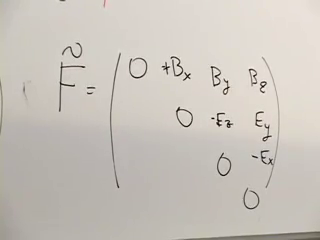
\includegraphics[width=0.58\textwidth]{lecture_58_figure_07.png}
\caption{必要な符号とともに電場と磁場の成分を交換して組み立てられる双対テンソル。}
\lectureframe{00:35:45}
\end{figure}

\section{共変形の真空方程式}

各マクスウェル方程式は1つの微分を含む。2階のテンソルから出発し、1つの微分添字を縮約すると1つの自由添字が残るので、自然な共変的候補は
\begin{align}
\partial_\mu F^{\mu\nu}&=0,
\label{eq:maxwell-covariant-vac}\\
\partial_\mu\widetilde F^{\mu\nu}&=0.
\label{eq:maxwell-dual-vac}
\end{align}
である。\(\nu\)の各固定値に対して、式~\eqref{eq:maxwell-covariant-vac}は1つの方程式である。\(\nu\)は\(t,x,y,z\)であり得るので、これは4つのスカラー方程式をまとめたものである。式~\eqref{eq:maxwell-dual-vac}は残りの4つをまとめたものである。これは元のリストにおける2つのベクトル回転方程式と2つのスカラー発散方程式に対応する。

簡潔な記法は、それがよく知られた方程式を再現する場合にのみ有用である。\(\nu=z\)とすると、
\begin{align}
\partial_\mu F^{\mu z}
&=\partial_tF^{tz}
  +\partial_xF^{xz}
  +\partial_yF^{yz}
  +\partial_zF^{zz}\\
&=-\partial_tE_z+\partial_xB_y-\partial_yB_x\\
&=-\partial_tE_z+
  \bigl(\boldsymbol\nabla\times\mathbf B\bigr)_z.
\end{align}
項\(F^{zz}\)は反対称性により消える。結果をゼロと置くと、
\begin{equation}
\boldsymbol\nabla\times\mathbf B=\partial_t\mathbf E.
\end{equation}
の\(z\)成分が得られる。\(x\)成分と\(y\)成分は添字を巡回させることで従う。

\begin{figure}[H]
\centering
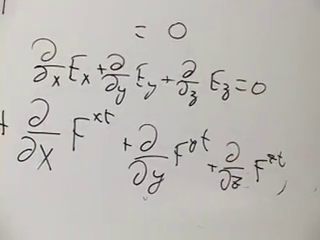
\includegraphics[width=0.76\textwidth]{lecture_58_figure_08.png}
\caption{共変場の方程式の成分展開。対角テンソル成分は消え、残りの項がマクスウェル方程式を再構成する。}
\lectureframe{00:43:30}
\end{figure}

次に時間成分を取る：
\begin{align}
\partial_\mu F^{\mu t}
&=\partial_tF^{tt}
  +\partial_xF^{xt}
  +\partial_yF^{yt}
  +\partial_zF^{zt}\\
&=\partial_xE_x+\partial_yE_y+\partial_zE_z\\
&=\boldsymbol\nabla\cdot\mathbf E.
\end{align}
したがってこれは式~\eqref{eq:gauss-e-vac}を与える。双対テンソルについて同じ検査を行うと、
\(\boldsymbol\nabla\cdot\mathbf B=0\) および
\(\boldsymbol\nabla\times\mathbf E=-\partial_t\mathbf B\) が得られる。

簡潔な方程式は今や単に推測されたのではなく確立された。それらの自由添字構造はそれらを4元ベクトル方程式にするので、ローレンツ変換はそれらの成分を変えるが形は変えない。これが、真空マクスウェル方程式がすべての慣性系で同じであるという正確な意味である。

\section{一次方程式から波動へ}

マクスウェル方程式は1階微分のみを含むのに対し、波動方程式は2階微分を含む。この見かけの不一致は、マクスウェルの理論が2つの場を結合するために解消される。\(\mathbf E\)と\(\mathbf B\)に対する1階方程式の対は、どちらか一方の場だけに対する2階方程式に組み合わせることができる。

式~\eqref{eq:ampere-vac}を時間で微分する：
\begin{equation}
\partial_t^2\mathbf E
=\boldsymbol\nabla\times\partial_t\mathbf B.
\end{equation}
ファラデーの法則が\(\mathbf B\)の時間微分を与え、
\begin{equation}
\partial_t\mathbf B=-\boldsymbol\nabla\times\mathbf E,
\end{equation}
したがって
\begin{equation}
\partial_t^2\mathbf E
=-\boldsymbol\nabla\times
  \bigl(\boldsymbol\nabla\times\mathbf E\bigr).
\label{eq:double-curl}
\end{equation}

黒板では記憶した恒等式を呼び出すのではなく、1つの成分を計算する。\(x\)成分について、
\begin{align}
\bigl[\boldsymbol\nabla\times
(\boldsymbol\nabla\times\mathbf E)\bigr]_x
&=\partial_y(\boldsymbol\nabla\times\mathbf E)_z
 -\partial_z(\boldsymbol\nabla\times\mathbf E)_y\\
&=\partial_y(\partial_xE_y-\partial_yE_x)\\
&\quad-\partial_z(\partial_zE_x-\partial_xE_z)\\
&=\partial_x(\partial_yE_y+\partial_zE_z)
 -\partial_y^2E_x\\
&\quad-\partial_z^2E_x.
\end{align}
\(\partial_x^2E_x\)を加えて引くことで発散をあらわにする：
\begin{align}
\bigl[\boldsymbol\nabla\times
(\boldsymbol\nabla\times\mathbf E)\bigr]_x
&=\partial_x(\boldsymbol\nabla\cdot\mathbf E)
 -\nabla^2E_x.
\label{eq:double-curl-x}
\end{align}
真空中では\(\boldsymbol\nabla\cdot\mathbf E=0\)。式~\eqref{eq:double-curl}と\eqref{eq:double-curl-x}を組み合わせると
\begin{equation}
\left(\partial_t^2-\nabla^2\right)E_x=0.
\label{eq:ex-wave}
\end{equation}

\begin{figure}[H]
\centering
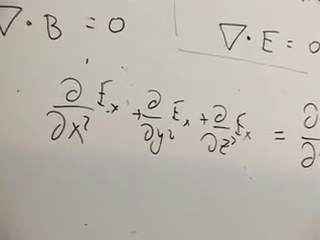
\includegraphics[width=0.72\textwidth]{lecture_58_figure_09.png}
\caption{成分計算により\(E_x\)に対する波動方程式に到達する。}
\lectureframe{00:57:10}
\end{figure}

同じ計算が\(E_y\)と\(E_z\)にも適用され、同様の消去により
\begin{equation}
\left(\partial_t^2-\nabla^2\right)\mathbf B=0.
\end{equation}
が得られる。したがって電場と磁場は真空中を波として伝播することができる。ここで用いた単位ではそれらの速さは1であり、これは通常の単位に戻すと速さが\(c\)であることを意味する。

\section{平面波とその偏光}

正の\(z\)方向に進む単純な波を構成する：
\begin{equation}
\mathbf E(z,t)
=\widehat{\mathbf x}\,E_0
  \cos\!\bigl(k(z-t)\bigr).
\label{eq:plane-e}
\end{equation}
そのプロファイルは形を変えずに\(z\)に沿って平行移動する。電場が\(x\)軸に沿って向くので、波は\(x\)方向に直線偏光している。例を単純に保つために\(E_y=0\)を選んだだけであり、第2の横偏光を含めることもできた。

縦成分は同じようには自由ではない。波は\(z\)と\(t\)のみに依存するので、
\begin{equation}
\boldsymbol\nabla\cdot\mathbf E
=\partial_zE_z=0.
\end{equation}
したがって\(E_z\)は定数であり得るが、変動する波のプロファイルを含むことはできない。一様な背景場は独立に重ね合わせたり取り除いたりできる；それは伝播する放射の一部ではない。波自体は横波である：
\begin{equation}
\mathbf E_{\mathrm{wave}}\cdot\widehat{\mathbf z}=0.
\end{equation}

ファラデーの法則が磁場を定める。式~\eqref{eq:plane-e}に対して、\(\boldsymbol\nabla\times\mathbf E\)の唯一の非零成分は\(y\)成分であり、
\begin{equation}
(\boldsymbol\nabla\times\mathbf E)_y=\partial_zE_x.
\end{equation}
したがって\(\partial_t\mathbf B\)は\(y\)に沿って向き、整合する選択は
\begin{equation}
\mathbf B(z,t)
=\widehat{\mathbf y}\,E_0
  \cos\!\bigl(k(z-t)\bigr).
\label{eq:plane-b}
\end{equation}
である。これらの単位では電場と磁場の振幅は等しい。それらの向きは
\begin{equation}
\mathbf E\perp\mathbf B,
\qquad
\mathbf E\perp\widehat{\mathbf z},
\qquad
\mathbf B\perp\widehat{\mathbf z},
\qquad
\mathbf E\times\mathbf B\parallel\widehat{\mathbf z}.
\end{equation}
に従う。

\begin{figure}[H]
\centering
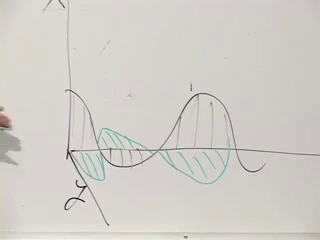
\includegraphics[width=0.70\textwidth]{lecture_58_figure_05.png}
\caption{横電磁波の完成した黒板スケッチ：電場と磁場の振動は互いに垂直であり、伝播方向にも垂直である。}
\lectureframe{01:05:25}
\end{figure}

\begin{figure}[H]
\centering
\scalebox{0.90}{%
\begin{tikzpicture}[x=1cm,y=1cm,>=Latex]
  \draw[->,thick] (0,0) -- (8.2,0) node[right] {$z$};
  \draw[->,thick] (0,-1.6) -- (0,1.7) node[above] {$x$};
  \draw[->,thick] (0,0) -- (-1.15,-0.8) node[below left] {$y$};
  \draw[blue!70!black,thick,domain=0:7.5,samples=120]
    plot (\x,{0.95*sin(90*\x)});
  \foreach \z/\s in {0.8/1,2.8/-1,4.8/1,6.8/-1}{
    \draw[->,green!45!black,thick]
      (\z,0) -- ++({-0.55*\s},{-0.38*\s});
  }
  \node[blue!70!black] at (6.9,1.25) {$\mathbf E$};
  \node[green!45!black] at (5.2,-1.05) {$\mathbf B$};
  \draw[->,very thick] (6.2,1.55) -- (7.7,1.55)
    node[midway,above] {propagation};
\end{tikzpicture}
}
\caption{場\(\mathbf E\)と\(\mathbf B\)は互いに垂直であり、伝播方向にも垂直である。}
\end{figure}

これが光および真空中のすべての電磁放射の特徴である。波を生み出した方程式がローレンツ共変であるので、別の慣性観測者もまた、\(c\)で進み、横方向の電場と磁場をもつ電磁波を記述する。

\section{電荷密度と電流密度}

ここで、一時的に脇に置いていた源を復元する。多数の荷電粒子が領域を占めるとき、それらを連続的な電荷密度に粗視化すると便利である。
\begin{equation}
\rho(\mathbf x,t)=\frac{dQ}{dV}.
\end{equation}
この近似は、水が分子から成るにもかかわらず連続的な流体として扱うことに似ている。正電荷と負電荷は逆の符号で寄与するので、\(\rho\) は単位体積あたりの正味の電荷である。

選んだ領域 \(V\) 内の電荷は
\begin{equation}
Q_V(t)=\int_V\rho(\mathbf x,t)\,dV.
\label{eq:charge-volume}
\end{equation}
である。密度は位置と時間によって変化しうる。電荷の山はある点から離れて移動し、そこでの局所的な密度を変化させうる。しかし、それが任意の仕方で変化することはできない。自然は電荷を保存する。

大域的な保存だけでは弱すぎる。それは、全電荷が変わらないまま、電荷が地球から消えて同時に火星に現れることを許してしまう。より強い主張は局所的なものである。電荷は、一つの場所を離れて別の場所に到達するには、その間の空間における流れを通じてのみ可能である。

その流れを記述するために、無限小の向き付けられた面要素
\begin{equation}
d\boldsymbol\sigma=\widehat{\mathbf n}\,d\sigma.
\end{equation}
を取る。その大きさは面積であり、その向きは面に垂直である。電流密度 \(\mathbf J\) は、単位時間あたりにその要素を横切る電荷が
\begin{equation}
\frac{dQ}{dt}=\mathbf J\cdot d\boldsymbol\sigma.
\label{eq:current-flux-element}
\end{equation}
となるように定義される。\(\mathbf J\) の大きさは単位面積・単位時間あたりの電荷であり、その向きは正電荷の流れの向きである。

\begin{figure}[H]
\centering
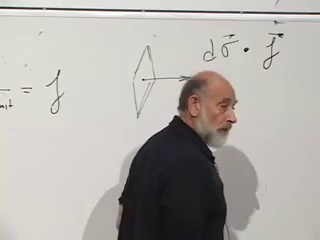
\includegraphics[width=0.64\textwidth]{lecture_58_figure_10.png}
\caption{向き付けられた面積要素とフラックス因子 \(d\boldsymbol\sigma\cdot\mathbf J\)。}
\lectureframe{01:18:15}
\end{figure}

内積は面に垂直な成分を選び出す。面に接する電流はどちらの側も横切らず、寄与はゼロである。法線に平行な電流は、大きさを固定すれば最大のフラックスを与える。導線の電流は一つの特別な場合であるが、\(\mathbf J\) はシートを通って流れる電荷や三次元空間全体を流れる電荷も記述しうる。

\section{局所保存と連続の方程式}

空間内の領域 \(V\) を固定し、その閉境界 \(\partial V\) のすべての要素を外向きに配向する。正味の外向き電流があれば、内部の電荷は減少する：
\begin{equation}
\frac{dQ_V}{dt}
=-\oint_{\partial V}\mathbf J\cdot d\boldsymbol\sigma.
\label{eq:integral-conservation}
\end{equation}
負号は慣習ではなく物理的である。正の外向きフラックスは領域から正電荷を取り除く。式~\eqref{eq:charge-volume} を用いると、
\begin{equation}
\int_V\partial_t\rho\,dV
=-\oint_{\partial V}\mathbf J\cdot d\boldsymbol\sigma.
\label{eq:integral-continuity-one}
\end{equation}

\begin{figure}[H]
\centering
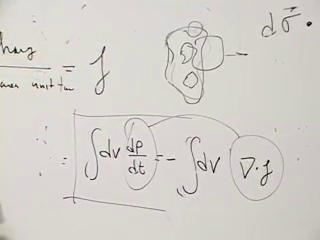
\includegraphics[width=0.72\textwidth]{lecture_58_figure_11.png}
\caption{表面フラックスを体積に関する表現に変換した後の固定領域の保存則。}
\lectureframe{01:29:00}
\end{figure}

ガウスの定理は、発散定理とも呼ばれ、閉曲面を通るフラックスとその内部の発散を関係づける：
\begin{equation}
\oint_{\partial V}\mathbf A\cdot d\boldsymbol\sigma
=\int_V\boldsymbol\nabla\cdot\mathbf A\,dV.
\label{eq:divergence-theorem}
\end{equation}
容器の内部の点で水を注入する隠れたパイプを思い描くことができる。発散は、パイプの端から水が現れる局所的な割合を測り、面積分は容器を出る水の総量を測る。内部で外向きの流れとして生成されるものは、最終的に境界を横切らなければならない。

式~\eqref{eq:divergence-theorem} を \(\mathbf J\) に適用すると
\begin{equation}
\int_V
\left(\partial_t\rho+\boldsymbol\nabla\cdot\mathbf J\right)dV=0.
\end{equation}
が得られる。この関係はあらゆる可能な領域 \(V\) に対して成り立つ。したがって被積分関数は点ごとに消えなければならない：
\begin{equation}
\boxed{\partial_t\rho+\boldsymbol\nabla\cdot\mathbf J=0.}
\label{eq:continuity-three}
\end{equation}

\begin{figure}[H]
\centering
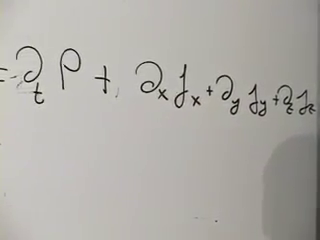
\includegraphics[width=0.72\textwidth]{lecture_58_figure_12.png}
\caption{成分ごとに書いた局所的な連続の方程式。}
\lectureframe{01:29:50}
\end{figure}

式~\eqref{eq:continuity-three} は、局所保存が要求することを正確に述べている。ある点または小さな領域内で電荷密度が減少するならば、電流はそこから外向きに発散しなければならない。電流が内向きに収束するならば、電荷密度は増加する。

密度と電流は自然に四元電流
\begin{equation}
J^\mu=(\rho,J_x,J_y,J_z)
\label{eq:four-current}
\end{equation}
を \(c=1\) 単位で形成する。連続の方程式はローレンツスカラー方程式
\begin{equation}
\partial_\mu J^\mu=0.
\label{eq:continuity-four}
\end{equation}
となる。相対論的な分布の流れは、一つの粒子の四元速度がそうであるように、四元ベクトルとして変換されるべきである。式~\eqref{eq:continuity-four} は、局所的な電荷保存をすべての慣性系で有効にする。

\section{源を含むマクスウェル方程式}

電荷と電流を復元すると
\begin{align}
\boldsymbol\nabla\cdot\mathbf E&=\rho,
\label{eq:gauss-e-source}\\
\boldsymbol\nabla\cdot\mathbf B&=0,\\
\boldsymbol\nabla\times\mathbf E&=-\partial_t\mathbf B,\\
\boldsymbol\nabla\times\mathbf B&=\partial_t\mathbf E+\mathbf J.
\label{eq:ampere-source}
\end{align}
が得られる。電気的な源を含む方程式は
\begin{equation}
\boxed{\partial_\mu F^{\mu\nu}=J^\nu,}
\label{eq:maxwell-source-covariant}
\end{equation}
にまとまり、源のない磁気的な対は
\begin{equation}
\boxed{\partial_\mu\widetilde F^{\mu\nu}=0.}
\label{eq:maxwell-dual-source}
\end{equation}
のままである。

\begin{figure}[H]
\centering
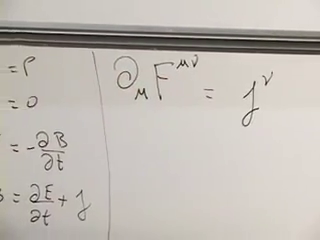
\includegraphics[width=0.78\textwidth]{lecture_58_figure_13.png}
\caption{源を含むマクスウェル方程式とその共変形 \(\partial_\mu F^{\mu\nu}=J^\nu\)。}
\lectureframe{01:34:00}
\end{figure}

式~\eqref{eq:maxwell-source-covariant} の時間成分は
\begin{equation}
\partial_\mu F^{\mu t}=J^t=\rho,
\end{equation}
と読め、すでに行った成分計算によりその左辺は
\(\boldsymbol\nabla\cdot\mathbf E\) となる。三つの空間成分は
\(\boldsymbol\nabla\times\mathbf B=\partial_t\mathbf E+\mathbf J\)
を再現する。

有用な整合性の検査もある。\(\partial_\nu\) を
式~\eqref{eq:maxwell-source-covariant} に適用すると
\begin{equation}
\partial_\nu J^\nu
=\partial_\nu\partial_\mu F^{\mu\nu}=0,
\end{equation}
が得られる。なぜなら二つの導関数は \(\mu\leftrightarrow\nu\) の下で対称であるのに対し、\(F^{\mu\nu}\) は反対称だからである。\editorialnote{この短い整合性の検査は共変方程式から従い、マクスウェル方程式が源を含む形で連続の方程式を自動的に尊重する理由を明示する。}

相反構造はこれで完成した。テンソル的な力の法則
\(f^\mu=qF^\mu{}_\nu u^\nu\) は場が電荷にどのように作用するかを記述し、
式~\eqref{eq:maxwell-source-covariant} は電荷と電流が場をどのように生成するかを記述する。両者はテンソル方程式である。真空中では、同じ場の方程式から \(c\) で進む横波が得られる。したがって、ローレンツ共変性と電磁波方程式は、この構成の動機となった点で一致する。すなわち、すべての慣性観測者が同じ電磁気学の法則と同じ光速度を得るのである。
\chapter{固有時、時間の遅れ、長さの収縮}

我々はしばしば光速が$c=1$である単位系を選ぶ。この単位系では、年で表した時間と光年で表した距離を直接比較でき、式はずっと読みやすくなる。$c$が物理的に重要になる場合は常に、それを復元する。次元解析だけでそれを特定するのに十分である。

\section{ガリレイ的時空格子}

静止系と、$x$軸に沿って速度$v$で運動する列車との間のアインシュタイン以前の関係から始めよう：
\begin{align}
x' &= x-vt, & t'&=t.
\label{eq:l4-galilean}
\end{align}
第2の式にはニュートンの絶対時間の仮定が含まれている。空間原点が互いに相対的に動いていても、すべての観測者は同じ同時刻のスライスを用いる。

プライムなしの観測者が線路のそばに立ち、プライム付きの観測者が列車に乗っているとしよう。列車の原点は$x'=0$であるから、プライムなし座標におけるその世界線は
\begin{equation}
x=vt.
\end{equation}
である。この傾いた直線が$t'$軸である。対照的に、$t'=t$は、$t'$が一定のすべての直線が$t$が一定の直線と同じ水平線であることを述べている。

\begin{figure}[H]
\centering
\includegraphics[width=0.72\textwidth]{lecture_04_figure_02.png}
\caption{ガリレイ変換と初期の$t$-$x$格子。運動する原点は$x=vt$を描くが、二つの系は共通の等時間線を保つ。}
\lectureframe{00:03:06}
\end{figure}

式~\eqref{eq:l4-galilean}をプライムなし座標について解くと
\begin{align}
x&=x'+vt'=x'+vt, & t&=t'.
\end{align}
が得られる。逆変換は$v$を$-v$に置き換えた同じ形をしている。列車が駅に対して前進するなら、駅は列車に対して後退する。この相互性は特殊相対性理論でも生き残るが、絶対時間は生き残らない。

\section{ローレンツ補正}

ガリレイ変換は、すべての慣性系で光速を同じにすることはできない。修正された関係は、まず$c=1$単位で、
\begin{align}
x'&=\frac{x-vt}{\sqrt{1-v^2}}, &
t'&=\frac{t-vx}{\sqrt{1-v^2}}.
\label{eq:l4-lorentz-natural}
\end{align}
である。通常の単位を復元すると
\begin{align}
x'&=\frac{x-vt}{\sqrt{1-v^2/c^2}}, &
t'&=\frac{t-vx/c^2}{\sqrt{1-v^2/c^2}}.
\label{eq:l4-lorentz-c}
\end{align}
となる。

\begin{figure}[H]
\centering
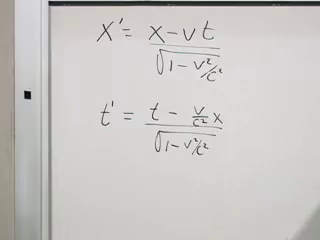
\includegraphics[width=0.74\textwidth]{lecture_04_figure_05.png}
\caption{$c$の因子を復元したローレンツ変換。}
\lectureframe{00:09:10}
\end{figure}

$v\ll c$では、ニュートン力学が用いられる状況において$v^2/c^2$と$vx/c^2$はどちらも微小である。そのとき式~\eqref{eq:l4-lorentz-c}はガリレイ的結果に帰着する。相対性理論はニュートン的運動学を捨て去るのではなく、その有効範囲を特定するのである。

$v=c$では、分母が消える。一つの慣性系が別の慣性系に対して光速で運動することはできない。その極限より十分下では補正は小さいが、その近くでは$x$と$t$の混合が避けられなくなる。

運動は$x$に沿って選ばれたので、横方向の座標は変化しない：
\begin{equation}
y'=y,\qquad z'=z.
\end{equation}
その理由を見る一つの方法は、列車とプラットフォームに同一の横方向の物差しを置くことである。二つの系の中間を運動する観測者は、棒が等しく反対向きの速度で近づいてくるのを見る。この設定には、一方の横方向の棒を他方より短くしうる特徴が何もない。

\section{光円錐に沿ったローレンツ変換}

式~\eqref{eq:l4-lorentz-natural}を読む幾何学的な方法がある。その二つの式を加える：
\begin{align}
t'+x'
&=\frac{(t-vx)+(x-vt)}{\sqrt{1-v^2}}\\
&=(t+x)\frac{1-v}{\sqrt{1-v^2}}\\
&=(t+x)\sqrt{\frac{1-v}{1+v}}.
\label{eq:l4-null-plus}
\end{align}
補完的な順序で引く：
\begin{align}
t'-x'
&=\frac{(t-vx)-(x-vt)}{\sqrt{1-v^2}}\\
&=(t-x)\frac{1+v}{\sqrt{1-v^2}}\\
&=(t-x)\sqrt{\frac{1+v}{1-v}}.
\label{eq:l4-null-minus}
\end{align}

\begin{figure}[H]
\centering
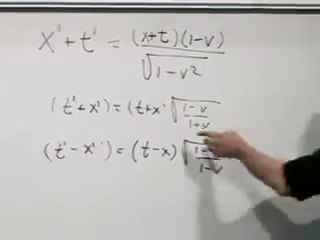
\includegraphics[width=0.75\textwidth]{lecture_04_figure_06.png}
\caption{ローレンツ変換をヌル結合$t+x$と$t-x$で書き直したもの。それらのスケール因子は互いに逆数である。}
\lectureframe{00:18:45}
\end{figure}

結合$t+x$と$t-x$は、二つの$45^\circ$光的方向に沿った座標である。ブーストはこれらの方向の一方を縮め、他方を逆因子で伸ばす。どちらかを$45^\circ$から回転させて離すことはない。したがって光線は光線のままであり、これが光速不変の時空的な描像である。

\begin{classroomqa}
\audiencequestion{中間の観測者は対称な実験を見るが、それによって列車とプラットフォームの観測者に対する結果がどのように確立されるのか。\lecturetimestamp{00:20:48}}
\lecturerresponse{もう一つの事実が用いられている：事象の一致は不変である。棒の端が出会うなら、その出会いは一つの時空事象である。すべての慣性観測者はそれに異なる座標を割り当ててよいが、一つの一致を二つの異なる位置に分けることはできない。対応する端点が出会う場所で発せられる閃光は、それらの事象を操作的に検出可能にする。中間系の対称性と二つの端点一致の不変性が、横方向の長さが一致することを確立する。}
\end{classroomqa}

\begin{classroomqa}
\audiencequestion{中間の慣性系を代表する自転車乗りは、棒の中点に物理的に位置していなければならないのか。\lecturetimestamp{00:22:25}}
\lecturerresponse{いいえ。基準系とは観測者と時計からなる一つの網全体であり、ある一点にある一つの目ではない。自転車乗りは端点の発光を後で受け取り、それらがどこから発せられたかを推論してもよい。重要なのは各発光事象の時空上の位置であり、光が最終的にどこで受信されるかではない。}
\end{classroomqa}

逐次的な速度の合成も同じ変換のもう一つの帰結であるが、それは意図的に次の講義に残される。現在の課題は、運動する時計が測る不変量を特定することである。

\section{不変間隔}

通常のデカルト軸の回転では、量$x^2+y^2$は不変である。ローレンツ変換は異なる二次形式を保存する。式~\eqref{eq:l4-lorentz-natural}より、
\begin{align}
t'^2-x'^2
&=\frac{(t-vx)^2-(x-vt)^2}{1-v^2}\\
&=\frac{t^2-2vtx+v^2x^2-x^2+2vtx-v^2t^2}{1-v^2}\\
&=t^2-x^2.
\label{eq:l4-interval}
\end{align}
混合項は相殺され、残った分子は共通因子$1-v^2$を含む。

\begin{figure}[H]
\centering
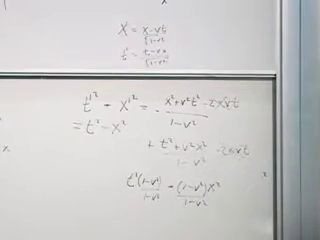
\includegraphics[width=0.76\textwidth]{lecture_04_figure_07.png}
\caption{$t'^2-x'^2=t^2-x^2$の板書による導出。}
\lectureframe{00:33:15}
\end{figure}

3つの空間次元がある場合、不変量は
\begin{equation}
t'^2-x'^2-y'^2-z'^2=t^2-x^2-y^2-z^2
\end{equation}
であり、$c=1$単位で表される。より一般には、2つの事象に対して座標差を用いる：
\begin{equation}
\Delta s^2
=c^2\Delta t^2-\Delta x^2-\Delta y^2-\Delta z^2.
\label{eq:l4-spacetime-interval}
\end{equation}
すべての慣性観測者は、その時間項と空間項を別々には一致させないが、この数については一致する。

\section{固有時と運動する時計}

光信号を交換して同期された時計を持つ静止観測者の格子を想像せよ。それらの読みは座標時$t$を定義する。次に、一つの腕時計をその格子の中を運んでいこう。その時計自身の読みは世界線に沿って時計に従う。その読みが固有時である。

時間的に分離された2つの事象に対して、
\begin{equation}
c^2\Delta\tau^2
=c^2\Delta t^2-\Delta x^2-\Delta y^2-\Delta z^2.
\label{eq:l4-proper-time}
\end{equation}
と定義する。$c=1$である1つの空間次元では、これは単に
\begin{equation}
\Delta\tau=\sqrt{\Delta t^2-\Delta x^2}.
\end{equation}
となる。平方根は通常の距離の公式と類似しているが、マイナス符号が幾何学を変える。

3つの場合がある：
\begin{align}
\Delta t^2-\Delta x^2 &>0 &&\text{timelike},\\
\Delta t^2-\Delta x^2 &=0 &&\text{lightlike},\\
\Delta t^2-\Delta x^2 &<0 &&\text{spacelike}.
\end{align}
光円錐の内部では固有時は実である。光円錐上では、$x=\pm t$であり、事象が一致する必要はないにもかかわらず、固有時はゼロである。光線はまさにそのような事象を結ぶことができる。光円錐の外部では分離は空間的であり、虚数の時計時間よりも実の固有距離$\sqrt{\Delta x^2-\Delta t^2}$で記述する方がよい。

\begin{figure}[H]
\centering
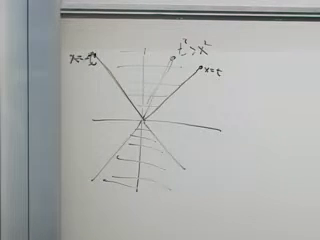
\includegraphics[width=0.73\textwidth]{lecture_04_figure_08.png}

\vspace{0.8em}

\begin{tikzpicture}[x=1.0cm,y=1.0cm]
\draw[->] (-3.3,0) -- (3.3,0) node[right] {$x$};
\draw[->] (0,-0.4) -- (0,4.0) node[above] {$t$};
\draw[thick] (0,0) -- (3.0,3.0) node[above right] {$x=t$};
\draw[thick] (0,0) -- (-3.0,3.0) node[above left] {$x=-t$};
\node at (0,2.0) {timelike};
\node at (2.25,1.05) {spacelike};
\node at (-2.25,1.05) {spacelike};
\end{tikzpicture}
\caption{板書の光円錐と、時間的、光的、空間的分離の明確な分類。}
\lectureframe{00:38:40}
\end{figure}

なぜ式~\eqref{eq:l4-proper-time}は時計の読みに等しいのか。静止している時計では$\Delta x=0$なので、$\Delta\tau=\Delta t$である。一様に運動する時計では、その時計が静止しているプライム付きの系を選ぶ。そこでは$\Delta x'=0$であり、不変性により
\begin{equation}
\Delta\tau
=\sqrt{\Delta t'^2-\Delta x'^2}
=\Delta t'.
\end{equation}
したがって、運動する時計は固有時を刻む。

\begin{classroomqa}
\audiencequestion{``事象間の間隔''と``時計の読み''は、同じものの2つの名前として使われているのか。
\lecturetimestamp{00:44:49}}
\lecturerresponse{理想的な時計が一方の事象から他方の事象へ慣性運動で進むとき、それらは一致する。不変間隔は幾何学的量であり、共動時計の端点の読みの差はその物理的測定である。静止した座標時計は一般に異なる座標時間間隔を記録する。}
\end{classroomqa}

\section{時間の遅れと同時性}

運動する系の原点を考えよ。その世界線は
\begin{equation}
x'=0,\qquad x=vt.
\end{equation}
に従う。同じ傾いた直線は、運動する時計の経路でもあり、$t'$軸でもある。

\begin{figure}[H]
\centering
\includegraphics[width=0.72\textwidth]{lecture_04_figure_03.png}
\caption{運動する原点：$x=vt$、$x'=0$、および$t'$軸は、同じ世界線の3つの記述である。}
\lectureframe{00:48:18}
\end{figure}

共通の原点とその世界線上の後の点との間に不変間隔を適用する：
\begin{align}
t'^2-x'^2&=t^2-x^2,\\
t'^2&=t^2-v^2t^2,\\
t'&=t\sqrt{1-v^2}.
\label{eq:l4-time-dilation-natural}
\end{align}
$c$を復元すると、
\begin{equation}
\Delta\tau=\Delta t\sqrt{1-\frac{v^2}{c^2}}
=\frac{\Delta t}{\gamma},
\qquad
\gamma=\frac{1}{\sqrt{1-v^2/c^2}}.
\label{eq:l4-time-dilation}
\end{equation}

\begin{figure}[H]
\centering
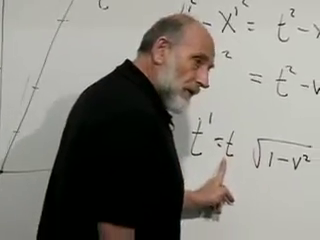
\includegraphics[width=0.73\textwidth]{lecture_04_figure_09.png}
\caption{板書の時間の遅れの結果：運動する時計は、$c=1$である単位で$t'=t\sqrt{1-v^2}$を蓄積する。}
\lectureframe{00:50:45}
\end{figure}

静止観測者は、運動する時計が遅れると言う。相互性により、運動する観測者も静止した時計について同じことを言わなければならない。2つの記述は異なる遠方の事象の対を比較するので、矛盾はない。

実際、式~\eqref{eq:l4-lorentz-natural}において$t'$が一定であることは
\begin{equation}
t-vx=\text{constant}.
\label{eq:l4-simultaneity}
\end{equation}
を満たす。運動する観測者の同時線は、水平線$t=\text{constant}$に対して傾いている。各観測者は、異なる遠方の時計の読みの集合を同時であると呼ぶ。その違いを可視化しておけば、時計の相互的な遅れは整合している。

\begin{figure}[H]
\centering
\begin{tikzpicture}[x=1cm,y=1cm]
\draw[->] (0,0) -- (0,4.2) node[above] {$t$};
\draw[->] (0,0) -- (5.2,0) node[right] {$x$};
\draw[thick,->] (0,0) -- (2.4,3.8) node[above] {$x'=0$};
\draw[dashed] (0,2.8) -- (4.8,2.8)
  node[right] {$t=\mathrm{const}$};
\draw[thick] (0.15,1.05) -- (4.7,2.35)
  node[right] {$t'=\mathrm{const}$};
\draw[thick] (3.4,0) -- (3.4,3.8);
\fill (3.4,2.8) circle (0.045);
\fill (3.4,1.98) circle (0.045);
\end{tikzpicture}
\caption{相互的な時間の遅れは、異なる同時面における時計の読みを比較する。}
\end{figure}

\section{双子の経路}

二人の双子が同じ事象から出発する。一方は$x=0$にとどまる。他方は速さ$v$で外へ向かって進み、向きを反転して同じ速さで戻る。再会したとき、彼らは時計として働きうるあらゆる物理過程を比較する。腕時計、心拍、代謝、あるいは老化そのものである。

旅行の各半分が、家にいる系で座標時間$T$かかるとする。家にいる双子の固有時間は
\begin{equation}
\tau_{\mathrm{home}}=2T.
\end{equation}
である。折り返しの事象の座標は$(vT,T)$である。したがって行きの脚は
\begin{align}
\tau_{\mathrm{leg}}
&=\sqrt{T^2-v^2T^2}
=T\sqrt{1-v^2}.
\end{align}
に寄与する。帰りの脚も同じ量に寄与するので、
\begin{equation}
\tau_{\mathrm{travel}}=2T\sqrt{1-v^2}<2T.
\label{eq:l4-twin}
\end{equation}
となる。

\begin{figure}[H]
\centering
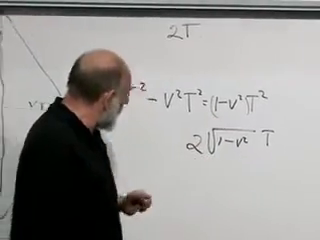
\includegraphics[width=0.73\textwidth]{lecture_04_figure_10.png}

\vspace{0.8em}

\begin{tikzpicture}[x=1.1cm,y=1cm]
\draw[->] (-0.2,0) -- (3.4,0) node[right] {$x$};
\draw[->] (0,-0.1) -- (0,4.4) node[above] {$t$};
\draw[very thick] (0,0) -- (0,4);
\draw[very thick] (0,0) -- (2.2,2) -- (0,4);
\draw[dashed] (0,2) -- (2.2,2);
\node[left] at (0,2) {$T$};
\node[left] at (0,4) {$2T$};
\node[below right] at (1.1,1.0) {$v$};
\node[above right] at (1.1,3.0) {$-v$};
\end{tikzpicture}
\caption{家にいる世界線と二つの旅行の脚。それらの固有時間が異なるのは、それらが時空を通る異なる経路だからである。}
\lectureframe{00:59:35}
\end{figure}

年齢が等しくないことに矛盾はない。旅行の経路は折り返しを含み、まっすぐな家の経路とは単一の慣性系の対称性によって関係づけられない。通常のユークリッド幾何学でも、二点間のまっすぐな経路と折れ曲がった経路は異なる長さをもつ。ミンコフスキー幾何学では、どちらの経路がより大きな間隔をもつかは逆になるが、比較は依然として幾何学的である。

\section{加速度と理想時計}

\begin{classroomqa}
\audiencequestion{折り返しでは物理が異なり、旅行者は加速する。それは時計の計算を無効にするのだろうか。
\lecturetimestamp{01:02:19}}
\lecturerresponse{加速度は実在し、非対称性を特定するのに役立つ。それを議論で消し去るべきではない。鋭い角は単に理想化された作図であり、有限の折り返しに丸めてもよい。さらなる物理的仮定は、十分に小さく、よく作られた時計は適度な加速度に敏感でなく、固有時間を記録し続けるというものである。大きな時計や壊れやすい時計は変形したり壊れたりするかもしれないが、それは時空間隔の欠陥ではなく、機構の欠陥である。}
\end{classroomqa}

この理想時計の仮定は、ローレンツ変換だけから導かれるものではない。それは実際の時計機構の振る舞いを通じて検証される。原子は、何百マイルもの大きさの時計よりもはるかに良い近似である。なぜなら、コンパクトな機構は加速度や重力のもとで歪みにくいからである。一般相対性理論の名を挙げても、この物理的問題は解消しない。選んだ機構がその環境にどう応答するかを、依然として知らなければならないのである。

\begin{classroomqa}
\audiencequestion{加速された軌道を、慣性解析が有効なままである短い区間に還元できるだろうか。\lecturetimestamp{01:09:08}}
\lecturerresponse{できる。曲線を短くほぼまっすぐな線分に分割し、各区間で固有時間を計算し、その結果を足し合わせる。これは、通常の曲線の長さを多くの小さな線分から求めることの時空版である。連続極限では、
\[
\tau=\int \sqrt{1-\frac{v(t)^2}{c^2}}\,dt,
\]
となる。これは、慣性座標系で記述された平坦な時空内の運動に対するものである。}
\end{classroomqa}

\section{双子が見るもの}

最終的な時計の読みは、光パルスを送ることによって操作的に定められる。両方の世界線上に固有時間の1秒間隔を印し、各双子が各印でパルスを放出するとする。行きの脚では、相手の双子から受け取るパルスは間隔が広がる。帰りの脚では、それらは詰まって到着する。これは時空図の上で直接表された相対論的ドップラー効果である。

\begin{figure}[H]
\centering
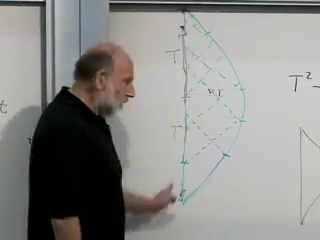
\includegraphics[width=0.73\textwidth]{lecture_04_figure_11.png}
\caption{家の世界線と旅行の世界線の間で交換される光信号。行きの脚でのまばらな到着と帰りの脚での圧縮された到着が、放出されたすべてのパルスを説明する。}
\lectureframe{01:12:55}
\end{figure}

この話のどの系も消え去らない。各観測者は最終的に相手が放出したすべてのパルスを受け取るが、その受信率は相対運動に依存する。行きの赤方偏移と帰りの青方偏移は、二つの経路にとって等しい持続時間の効果ではない。したがって、受け取ったすべてのパルスを数えることは固有時間の比較と一致する。

\begin{classroomqa}
\audiencequestion{戻ってくる旅行者が青方偏移した光を受け取るなら、旅行者は光源が放出したよりも多くのエネルギーを集められるだろうか。
\lecturetimestamp{01:13:50}}
\lecturerresponse{その問いには、エネルギーの相対論的定義と系依存性が必要であり、それらはまだ展開されていない。もっともではあるが、座標とパルス数だけでは、特に加速された観測者について、エネルギーの収支を決着させるのに十分ではない。したがって、答えは推測するのではなく後回しにすべきである。}
\end{classroomqa}

\section{閉じた空間方向}

\begin{classroomqa}
\audiencequestion{空間方向の一つがコンパクトであるとしよう。双子の一方はその方向に沿って一様に運動し、出発点に戻り、加速度をまったく避けることができるだろうか。そのとき、何が双子を区別するのか。\lecturetimestamp{01:15:14}}
\lecturerresponse{空間は、より大きな空間の中に曲げ込まれた一枚の紙としてではなく、内在的に円筒として想像されるべきである。動径方向の加速度は必要ない。それでも、戻ってくる観測者は、同じ場所が再び現れるという大域的な事実に遭遇する。これは非対称性を示しているが、完全な答えには、空間的同一視を伴う特殊相対性理論の注意深い取り扱いが必要である。この問いは、その場しのぎで答えるのではなく、ここでは未解決のままにしておく。}
\end{classroomqa}

\begin{figure}[H]
\centering
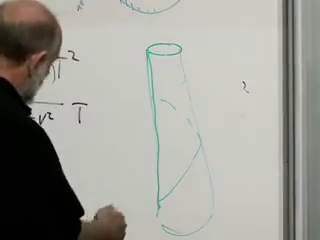
\includegraphics[width=0.72\textwidth]{lecture_04_figure_04.png}

\vspace{0.8em}

\begin{tikzpicture}[x=1cm,y=1cm]
\draw[thick] (0,0) ellipse (1.3 and 0.35);
\draw[thick] (-1.3,0) -- (-1.3,-3.1);
\draw[thick] (1.3,0) -- (1.3,-3.1);
\draw[thick] (0,-3.1) ellipse (1.3 and 0.35);
\draw[->,very thick] (0.0,0.38) arc (90:-210:1.38 and 0.42);
\node[right] at (1.65,-1.5) {compact spatial direction};
\end{tikzpicture}
\caption{黒板に描かれたコンパクト空間の問い。清潔な内在的円筒とともに。これは、余分な動径次元に埋め込まれた円筒の周りを運動することではなく、大域的同一視に関する問いである。}
\lectureframe{01:17:56}
\end{figure}

\section{長さは同時刻面で測られる}

特殊相対性理論の問題では、まず時空図を描く。プライムなしの系で静止しているメートル棒を取り、その端点を$x=0$と$x=1$に置く。時間が経つにつれて、二つの端点は垂直な世界線を描く。棒はそれらの間にリボンを掃き出す。

運動している観測者は、運動している時間$t'$の一つの値で両方の端点を測らなければならない。式~\eqref{eq:l4-simultaneity}から、原点を通り$t'=0$である面は、$c=1$単位で
\begin{equation}
t=vx
\end{equation}
を満たす。それは右の端点$x=1$と$t=v$で交わる。

\begin{figure}[H]
\centering
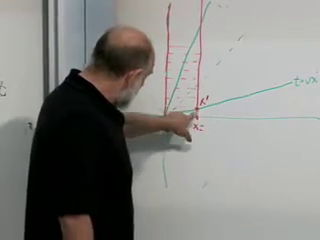
\includegraphics[width=0.73\textwidth]{lecture_04_figure_12.png}

\vspace{0.8em}

\begin{tikzpicture}[x=1.55cm,y=1.15cm]
\draw[->] (-0.5,0) -- (3.1,0) node[right] {$x$};
\draw[->] (0,0) -- (0,3.8) node[above] {$t$};
\draw[very thick,red] (0,0) -- (0,3.3);
\draw[very thick,red] (2.15,0) -- (2.15,3.3);
\fill[red!12] (0,0) rectangle (2.15,3.3);
\draw[very thick,green!50!black] (0,0) -- (1.2,3.1)
  node[above] {$x=vt$};
\draw[very thick,blue] (0,0) -- (2.15,1.15)
  node[right] {$t'=0$};
\fill (2.15,1.15) circle (0.045);
\node[right] at (2.22,1.35) {$(x,t)=(1,v)$};
\node[below] at (2.15,0) {$1$};
\end{tikzpicture}
\caption{静止している棒は時空のリボンを掃き出す。運動している観測者にとっての長さは、一つの$t'=\mathrm{const}$面におけるその端点間の隔たりである。}
\lectureframe{01:24:20}
\end{figure}

選ばれた端点の隔たりは空間的であるから、不変量の正の空間的形式を用いる：
\begin{equation}
x'^2-t'^2=x^2-t^2.
\end{equation}
選ばれた端点では、$t'=0$、$x=1$、そして$t=v$である。したがって
\begin{align}
x'^2&=1-v^2,\\
x'&=\sqrt{1-v^2}.
\end{align}
よって、静止長$L$は、運動している系で
\begin{equation}
L'=L\sqrt{1-v^2/c^2}=\frac{L}{\gamma}.
\label{eq:l4-length-contraction}
\end{equation}
と測られる。

\begin{figure}[H]
\centering
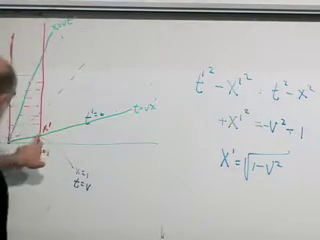
\includegraphics[width=0.76\textwidth]{lecture_04_figure_13.png}
\caption{完成した長さの収縮の作図と、単位静止長に対する黒板の結果$x'=\sqrt{1-v^2}$。}
\lectureframe{01:28:10}
\end{figure}

逆の主張もまた成り立つ：プラットフォームの観測者は、列車の縦方向のメートル棒により短い長さを割り当てる。ここでもまた、二人の観測者は異なる同時的な端点事象を選ぶので、相互性は矛盾ではない。

\section{最後の質問}

\begin{classroomqa}
\audiencequestion{光以外に光速で伝播するものはあるか。特に、重力はどうか。\lecturetimestamp{01:29:29}}
\lecturerresponse{一般相対性理論は、$c$で伝播する重力波を予言する。この講義の時点では、証拠は連星パルサーなどの系から間接的に得られており、重力波はまだ直接検出されていなかった。\editorialnote{実験状況はこの2006年の講義の後に変わった。LIGOは2015年にGW150914を直接検出し、2017年におけるGW170817とその電磁対応物の同時観測は、重力と光の伝播速度が$10^{15}$分の数以内で一致することを示した。\url{https://ligo.org/detections/gw150914/}と
\url{https://doi.org/10.1103/PhysRevLett.119.251302}を参照。}}
\end{classroomqa}

\begin{classroomqa}
\audiencequestion{宇宙飛行士は、何光年もの距離を、その距離を光年で表した値よりも短い固有時間で横切ることができるだろうか。それは光より速く動くことを意味するだろうか。\lecturetimestamp{01:30:38}}
\lecturerresponse{宇宙飛行士の固有時間は
$\sqrt{\Delta t^2-\Delta x^2}$であり、これは座標時間
$\Delta t$より小さい。宇宙飛行士の慣性系では、星々の間の距離はローレンツ収縮している。星々は速度$-v$で動いており、光より速くはない。横切るべき収縮した距離が単に小さいだけである。}
\end{classroomqa}

宇宙飛行士が静止から始めて加速する場合、記述は一連の瞬間的慣性系の間で変化する。星々に割り当てられる距離は、その移行の間に変化しうる。一つの固定したローレンツ変換を加速された全履歴に適用することはできないが、全固有時間は依然として世界線に沿った寄与を足し合わせることによって得られる。同じことは、巡航速度で生まれるのではなく、打ち上げ、方向転換、減速する現実的な双子にも当てはまる。

\begin{classroomqa}
\audiencequestion{これらの難問は、時間を特別なものとして扱うことから生じるのだろうか。それを第4の次元と呼ぶべきなのだろうか。\lecturetimestamp{01:36:43}}
\lecturerresponse{時間は第4の次元であるというスローガンから出発する必要はない。ローレンツ変換それ自体が空間と時間を混ぜ合わせることを強制する一方で、不変間隔$t^2-x^2-y^2-z^2$は、時間と空間で符号が異なる一つの幾何学の部分としてそれらを扱う。低速度ではこの混合は無視できるほどになり、おなじみのニュートン的な直観が戻ってくる。しかし相対論的な速度では、空間と時間を根本的に切り離されたものと見なすことはできない。}
\end{classroomqa}

したがって、時間の遅れ、長さの収縮、双子の比較、短縮された旅行時間は、別々のトリックではない。それらはすべて三つの習慣から導かれる。すなわち、比較している事象を特定し、それらの時空幾何学を描き、不変間隔を用いることである。

\chapter{火の玉、座標系、そして四元ベクトル}

高エネルギー衝突の議論から残った一つの問いから始めよう。二つの重い原子核の衝突は、静かな天体物理的黑洞ではなく、激しく変化する対象を生み出す。では、その衝突を事象の地平面によって記述することは何を意味しうるのか。その答えは、強結合物質の五次元的な描像、加速器に関するいくつかの実践的な問い、そして最終的には特殊相対性理論の幾何学へと導く。最後には、速度と運動量は四元ベクトルとなり、エネルギーは運動量の三成分と並ぶ位置を占めることになる。

\section{五次元の中の火の玉}

\begin{classroomqa}
\audiencequestion{衝突で生成される対象は不安定であり、形を変える。そのような複雑な対象を、どうしてブラックホールと呼べるのか。}
\lecturerresponse{床と天井の間に走る第五の空間方向を思い描こう。その方向の重力は励起を床へと引き寄せる。衝突はそこに高温のエネルギー塊を堆積させる。その塊は広がり形を変えるが、それでも地平面、温度、エントロピーを持ちうる。}
\end{classroomqa}

この五次元世界を運動する粒子、あるいはより絵画的には小さな弦を想像しよう。床へ落ちる励起は、四次元ではハドロンとして現れる。陽子、中性子、中間子、その他の拡がった複合対象である。天井の近くに付着した励起は、より素粒子的に現れる。したがって、垂直方向の位置はスケールを符号化する幾何学的な方法である。床は長距離のハドロン的領域を表し、天井は短距離の自由度を表す。

二つのハドロンが衝突すると、床の近くの二つの対象が互いにぶつかり、大量のエネルギーを撒き散らす。結果は剛体ではない。それは高温で地平面を伴う塊であり、五次元重力場の中のある種の水たまりである。それは通常の四次元空間における天体物理的黑洞でもなく、天井に付着したプランクスケールのブラックホールでもない。それは床の近くの強結合火の玉の重力による記述である。

高エネルギーでは、入射する原子核はローレンツ収縮して薄いパンケーキになる。それらは衝突し、小さな領域にエネルギーを堆積させ、平衡へと広がる流体を生成する。その小さな粘性は、クォーク--グルーオン・プラズマの驚くべき特徴の一つであった。五次元的な記述では、同じ発展が歪んだ地平面の緩和である。

\begin{figure}[H]
\centering
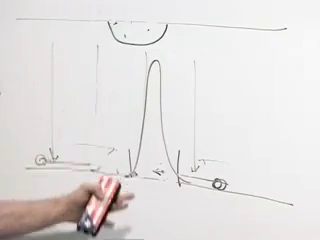
\includegraphics[width=0.82\textwidth]{lecture_05_figure_01.png}
\caption{第五次元の床と天井の描像。中心の地平面を伴う塊が、衝突後に床に沿って広がる。}
\lectureframe{00:04:22}
\end{figure}

地平面は永遠に残るわけではない。ホーキング放射がエネルギーを運び去り、四次元的な記述では、その放射は衝突から現れる通常のハドロンのシャワーである。検出器の事象における数千の飛跡は、この言葉では、双対ブラックホールから沸騰して出てくる粒子である。

\subsection{余分な次元は実在するのか。}

\begin{classroomqa}
\audiencequestion{第五の次元は空間的な次元であり、床と天井の間に描かれた線は文字通りその方向に延びているのか。}
\lecturerresponse{はい。それは空間的であり、その五次元幾何学に描かれた面は地平面である。余分な方向を``実在する''と呼ぶか、等価な数学的記述とみなすかは、より深い問いである。}
\end{classroomqa}

有用な主張は、重力が量子色力学を置き換えるということではない。むしろ、二つの言語が同じ物理を記述しうるということである。四次元的な言語では、通常の重力場を持たない、クォークとグルーオンの高温火の玉がある。五次元的な言語では、重力と地平面がある。対応が正しければ、正直なQCD計算と双対な重力計算は、両方が実行できるあらゆる場所で一致しなければならない。

\begin{classroomqa}
\audiencequestion{QCDには重力も地平面もない。ブラックホール描像は新しい物理を加えているのか、それとも単に火の玉を別の仕方で記述し直しているだけなのか。}
\lecturerresponse{四次元ではそれはクォークとグルーオンのプラズマであり、五次元的な姿では地平面を伴う重力による記述を持つ。利点は計算にある。強結合QCDは極めて難しいが、いくつかの地平面の性質---特に粘性---は比較的容易に計算できる。}
\end{classroomqa}

``実在の次元''と``数学的類推''の区別は、その記述が有用であるためにあらかじめ決着させる必要はない。ある構造は、他の変数とともに、より単純でより首尾一貫した法則の集合へと統合されるときに、物理的解釈を得る。とはいえ、事態を過大に述べるべきではない。観測されたクォーク--グルーオン・プラズマへのゲージ／重力双対性の応用は、強結合ダイナミクスの模型であって、現実世界のQCDが既知の厳密な重力双対をもつことの証明ではない。\editorialnote{この限定は、QCD応用の現代的な位置づけを明示するものであり、ここで展開した五次元の機構を変えるものではない。}

\section{なぜ衝突型加速器はビームを衝突させるのか}

ここで問いは実際的になる。なぜ単一のビームと静止標的ではなく、二つの運動するビームを用いるのか。なぜ円形加速器はそれほど大きいのか。なぜ電子と陽子は異なる扱いを受けるのか。これらの問いはすべて、相対論的エネルギーに関する問いである。

\begin{classroomqa}
\audiencequestion{なぜ一つの高エネルギー・ビームを静止標的に当てるのではなく、二つのビームを衝突させるのか。}
\lecturerresponse{新しい粒子を生み出すのは、重心系で利用可能なエネルギーである。等しく逆向きの二つの相対論的ビームは正味の運動量をもたないので、そのエネルギーの本質的にすべてが衝突に利用できる。固定標的では、入射エネルギーの多くが重心の運動として残ることを強いられる。}
\end{classroomqa}

大きさ\(p\)の逆向きの運動量をもつ二つの超相対論的粒子について、\(c=1\)単位での講義レベルの見積もりは
\begin{equation}
E_{\mathrm{cm}}^{\mathrm{collider}}\simeq 2p.
\end{equation}
である。対応する固定標的の見積もりは、ビーム運動量の平方根としてのみ増大する。
\begin{equation}
E_{\mathrm{cm}}^{\mathrm{fixed}}\sim \sqrt{mp}.
\end{equation}
重要なのは、省略された数因子ではなく、このスケーリングである。ビームエネルギーを二倍にすると衝突型加速器のエネルギーは二倍になるが、固定標的の重心エネルギーは平方根の分だけしか増加しない。

不変量の計算はこの比較を精密にする。\(P_1\)と\(P_2\)が入射四元運動量であるならば、
\begin{equation}
s=(P_1+P_2)^2,
\qquad E_{\mathrm{cm}}=\sqrt{s}.
\end{equation}
である。エネルギー\(E\)の等しい逆向きビームでは、空間的運動量が相殺し、\(\sqrt{s}=2E\)となる。エネルギー\(E\gg m\)の入射粒子が静止した等質量の標的に当たる場合、
\begin{equation}
s=2m^2+2mE,
\qquad
\sqrt{s}\simeq \sqrt{2mE}
\qquad (c=1).
\end{equation}
である。この短い不変量による導出は、口頭の見積もりで省略された因子を与える。\editorialnote{この導出は、講義のスケーリングの議論を再現可能にするために含められている。}

\begin{classroomqa}
\audiencequestion{円形加速器がこれほど大きくなくてはならない根本的な理由はあるのだろうか。同じビームを、より小さな装置の中でもっと何度も周回させることはできないのだろうか。}
\lecturerresponse{場と物質が限界を課す。粒子がメートルあたりに受け取るエネルギー増加は有限であるため、より高エネルギーの装置にはより大きな実効加速長が必要となる。また、きつい円はより大きな横方向の加速度を要求し、加速された電荷は放射する。リングが小さすぎれば、ビームは装置が供給するのと同じ速さでエネルギーを放射してしまう。}
\end{classroomqa}

曲げの関係は近似的に
\begin{equation}
p=qBR,
\end{equation}
である。したがって、磁場\(B\)を固定すれば、より大きな運動量\(p\)にはより大きな半径\(R\)が必要である。高周波空洞がビームエネルギーを高める仕事を行い、磁石がビームを曲げて集束する。広い教訓は黒板で与えられたもののままである。すなわち、場の強さと放射損失のため、任意に高エネルギーの加速器を小さなリングに圧縮することはできない。

円運動は、速さが一定でも速度が向きを変えるため加速度をもつ。加速された電荷はシンクロトロン放射を放出する。線形加速器は連続的な曲げによる損失を避けるが、短い加速の押し自体が文字通り放射を伴わないわけではない。円形機械は、同じ装置を各周回で再利用することと引き換えに、曲げのコストを受け入れる。

\begin{classroomqa}
\audiencequestion{なぜ電子はSLACの直線機械と結びつけられ、一方で円形高エネルギー衝突型加速器は陽子や他のハドロンを用いるのか。}
\lecturerresponse{電子ははるかに軽い。与えられた高エネルギーでは、そのローレンツ因子ははるかに大きく、円運動の加速度は電子をはるかに強く放射させる。より重い陽子は、シンクロトロン損失が手に負えなくなる前に、繰り返し周回して各周回でエネルギーを獲得できる。}
\end{classroomqa}

固定されたエネルギーとリング半径に対して、放射されるパワーは粒子質量とともに非常に急峻にスケールする。
\begin{equation}
P_{\mathrm{sync}}\propto \frac{E^4}{m^4R^2}.
\end{equation}
これが、電子--陽子の区別が、``軽い粒子の方が速く動く''という言葉が示唆するよりもはるかに鋭い理由である。両方のビームはすでに\(c\)に極めて近づき得るが、それらのローレンツ因子と放射損失は大きく異なる。\editorialnote{曲げの関係とシンクロトロンのスケーリングは、講義の定性的な加速器の議論を精密にする。それらは黒板では導出されなかった。}

\begin{classroomqa}
\audiencequestion{なぜハドロンも直線で加速しないのか。}
\lecturerresponse{それは可能である。困難は長さである。リングでは同じ粒子が加速構造を何度も通過する。等価な線形ハドロン機械は途方もなく長くなければならない。有用な妥協は大きなリングであり、陽子放射が許容できる程度に十分大きい。}
\end{classroomqa}

これらの加速器の問いは、ニュートンの規則がなぜ不十分であるかをまさに明らかにする。ここで特殊相対性理論に戻り、そのような比較を体系的にする言語を構築する。

\section{ガレージとリムジン}

約12フィートの長さのガレージと約20フィートの長さのストレッチリムジンを考える。運転手はリムジンがローレンツ収縮するまで加速し、それが収まることを期待する。ガレージの系では動いているリムジンは短いので、可能に見える。しかしリムジンの系では動いているガレージが短いので、不可能に見える。リムジン全体がガレージの中に入ることができるか。

壁との衝突が我々の注意をそらさないように、両方の扉を開ける。リムジンが中にあると言うことは、その前端と後端が\emph{同時に}中にあることを意味する。その最後の言葉にパズルのすべてが含まれている。

\(t\)を縦軸、\(x\)を横軸として時空図を描く。光線は\(c=1\)単位で\(45^\circ\)の光円錐を形成する。ガレージは静止しているので、その二つの扉の世界線は垂直である。リムジンの前端と後端は二本の平行な傾斜した世界線を描く。動いている系の\(t'\)軸は光円錐の方向に傾き、その同時線は傾いた\(x'\)軸に平行である。

\begin{figure}[H]
\centering
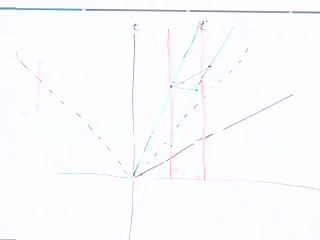
\includegraphics[width=0.82\textwidth]{lecture_05_figure_02.png}
\caption{完成したガレージ--リムジン時空図。垂直線がガレージを囲み、傾斜線がリムジンの両端を描く。水平および傾斜した切断は、二つの系の異なる同時スライスを表す。}
\lectureframe{00:31:05}
\end{figure}

ガレージの系では、水平線が二つのガレージ世界線の間で両方のリムジン世界線を横切ることができる。そのガレージ時刻では、後端は入っており、前端はまだ出ていない。収縮したリムジンは完全に中にある。

リムジンの系では、関連する同時事象は傾斜した線上にある。後端が入る事象を通るそのような線を描く。それは前端がすでに遠い扉を通過した後に前端世界線と交わる。リムジンはそれ自身の同時性によれば決して完全に中にはない。両方の主張は、異なる事象の対を比較しているので真である。

\begin{classroomqa}
\audiencequestion{二本の緑の世界線とそれらの間の水平線分は平行四辺形を形成するか。その黒い線分は車両の長さか。}
\lecturerresponse{水平線分はローレンツ収縮した長さである。なぜならその端点はガレージの系で同時だからである。固有長はリムジンの系で同時な端点から、\(x'\)に平行な線上で得られる。二つの測定は同じ世界線の対を通る異なる切断を用いる。}
\end{classroomqa}

\(L_0\)が固有長なら、水平なガレージ系の切断は長さ
\begin{equation}
L=\frac{L_0}{\gamma},
\qquad
\gamma=\frac{1}{\sqrt{1-v^2/c^2}}.
\end{equation}
を持つ。式だけではパラドックスを解決しない。図が解決する。なぜならどの事象が比較されたかを示すからである。相対性理論のパズルが二つの両立しない答えを生むように見えるときはいつでも、``同時に''の暗黙の使用を探せ。

\section{四つの座標と二つの添字位置}

パズルから運動法則へ移るために、幾何学を記憶する記法が必要である。座標を
\begin{equation}
(X^1,X^2,X^3,X^0)=(x,y,z,t),
\qquad X^\mu=(x,y,z,t),
\end{equation}
としてまとめる。ここで\(\mu\)は\(1,2,3,0\)を走る。この順序は、その添字が\(0\)であっても時間をページの最後に置き、黒板で用いられた慣習に一致する。

\begin{classroomqa}
\audiencequestion{我々は\(c=1\)と設定しているのか。通常の単位を復元すれば、時間座標は\(ct\)であるべきか。}
\lecturerresponse{はい。幾何学を展開する間は\(c=1\)と設定し、次元や非相対論的極限が問題になるときに\(c\)の因子を戻す。従来の長さの単位では、時間座標は\(ct\)である。}
\end{classroomqa}

同じベクトルは下付き添字で書くこともできる。ここで用いる符号の規約では、
\begin{equation}
X_\mu=(-x,-y,-z,t).
\end{equation}
したがって、添字を下げると3つの空間成分の符号が反転し、時間成分は変わらない。例えば、
\begin{equation}
X^\mu=(3,2,4,10)
\quad\Longrightarrow\quad
X_\mu=(-3,-2,-4,10).
\end{equation}
これらは2つの時空点ではなく、1つの幾何学的対象の2つの成分表示である。

\begin{classroomqa}
\audiencequestion{どの成分が共変でどれが反変か、また添字は上付きと下付きのどちらを意味するのか。}
\lecturerresponse{上付き添字の成分は反変であり、下付き添字の成分は共変である。教室で役立つ記憶法は``coは下、contraは上''である。物理学者はしばしば単に「上」と「下」と言う。}
\end{classroomqa}

この記法は不変な縮約
\begin{equation}
X_\mu X^\mu=t^2-x^2-y^2-z^2.
\label{eq:l5-interval}
\end{equation}
においてその価値を発揮する。微分形式ではこれは
\begin{equation}
d\tau^2=dt^2-dx^2-dy^2-dz^2
\qquad (c=1).
\label{eq:l5-proper-time}
\end{equation}
である。時間的運動では、\(d\tau\)は世界線に沿って動く時計が記録する時間である。

同じ添字が上に1回、下に1回現れるときはいつでも、和をとるものと理解される。アインシュタインの規約により
\begin{equation}
\sum_{\mu}X_\mu X^\mu
\end{equation}
は式~\eqref{eq:l5-interval}のより短い表現になる。これは単に活字上の節約ではない。ミンコフスキー幾何学の交代する符号が、あらゆる式で手作業で書き直されるのを防ぐのである。

\begin{classroomqa}
\audiencequestion{\(\tau\)は固有時間の標準的な記号か。}
\lecturerresponse{はい。記号\(s\)も使われることがあるが、\(\tau\)は固有時間の標準的な選択である。}
\end{classroomqa}

\section{容易な対称性としての回転}

ローレンツブーストは空間と時間を混ぜ合わせる。その行列を調べる前に、より馴染み深い空間軸の回転という操作を考えよう。相対運動が任意の方向を向いているなら、その方向が新しい\(x\)軸になるまで軸を回転させ、それから既知のブーストを適用すればよい。したがって回転は構成の一部であり、装飾的な回り道ではない。

\(z\)軸のまわりの角度\(\theta\)の回転では、
\begin{align}
x'&=x\cos\theta+y\sin\theta,\nonumber\\
y'&=-x\sin\theta+y\cos\theta,\label{eq:l5-rotation}\\
z'&=z.\nonumber
\end{align}
\(\theta=0\)ではこれらの式は\(x'=x\)と\(y'=y\)を与え、\(\theta=\pi/2\)では期待される符号で軸を交換する。

この変換はユークリッド距離を保つ。
\(c_\theta=\cos\theta\)および\(s_\theta=\sin\theta\)と書くと、
\begin{align}
x'^2+y'^2
&=(xc_\theta+ys_\theta)^2+(-xs_\theta+yc_\theta)^2\nonumber\\
&=x^2(c_\theta^2+s_\theta^2)
  +y^2(s_\theta^2+c_\theta^2)\nonumber\\
&\quad+2xyc_\theta s_\theta-2xyc_\theta s_\theta\nonumber\\
&=x^2+y^2.
\end{align}
交差項は相殺され、\(c_\theta^2+s_\theta^2=1\)となる。\(z'=z\)であるから、全長\(x^2+y^2+z^2\)は不変である。

同じ式は1つの行列方程式になる：
\begin{equation}
\begin{pmatrix}x'\\y'\\z'\end{pmatrix}
=
\underbrace{\begin{pmatrix}
\cos\theta&\sin\theta&0\\
-\sin\theta&\cos\theta&0\\
0&0&1
\end{pmatrix}}_{M}
\begin{pmatrix}x\\y\\z\end{pmatrix}.
\label{eq:l5-rotation-matrix}
\end{equation}
添字記法では、
\begin{equation}
x'^i=M^i{}_{j}x^j,
\qquad i,j=1,2,3.
\end{equation}

\begin{figure}[H]
\centering
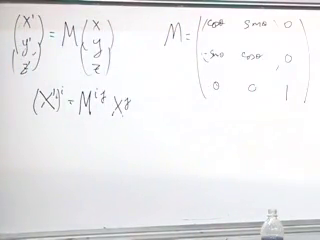
\includegraphics[width=0.82\textwidth]{lecture_05_figure_03.png}
\caption{行列方程式としても添字記法でも書かれた空間回転。}
\lectureframe{01:00:40}
\end{figure}

\section{ローレンツ行列と合成速度}

\(x\)に沿った運動について、\(c=1\)単位でのローレンツ変換は
\begin{align}
x'&=\gamma_v(x-vt), & y'&=y,\nonumber\\
z'&=z, & t'&=\gamma_v(t-vx),
\end{align}
ここで
\begin{equation}
\gamma_v=\frac{1}{\sqrt{1-v^2}}.
\end{equation}
成分の順序を\((x,y,z,t)\)とすると、これは
\begin{equation}
\begin{pmatrix}x'\\y'\\z'\\t'\end{pmatrix}
=
\begin{pmatrix}
\gamma_v&0&0&-\gamma_vv\\
0&1&0&0\\
0&0&1&0\\
-\gamma_vv&0&0&\gamma_v
\end{pmatrix}
\begin{pmatrix}x\\y\\z\\t\end{pmatrix}.
\label{eq:l5-lorentz-matrix}
\end{equation}
となる。

\begin{figure}[H]
\centering
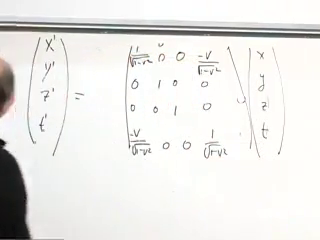
\includegraphics[width=0.82\textwidth]{lecture_05_figure_04.png}
\caption{\(4\times4\)ローレンツ行列。\(x\)成分と\(t\)成分だけが混ざり合い、\(y\)と\(z\)は変わらない。}
\lectureframe{01:04:40}
\end{figure}

行列の積が今や物理的な問いに答える。ある観測者が我々に対して速度\(v\)で運動し、第三の観測者がその観測者に対して速度\(u\)で運動しており、すべて同じ軸に沿っているとしよう。ニュートン力学の運動学では\(w=u+v\)を与え、それでは\(3c/4\)の2つの速度が合成されて\(3c/2\)になることが許されてしまう。相対性理論は異なる規則を与えなければならない。

ブーストの実質的な部分は\(2\times2\)行列
\begin{equation}
B(v)=\gamma_v
\begin{pmatrix}1&-v\\-v&1\end{pmatrix}.
\end{equation}
である。2つのブーストを合成すると
\begin{align}
B(u)B(v)
&=\gamma_u\gamma_v
\begin{pmatrix}1&-u\\-u&1\end{pmatrix}
\begin{pmatrix}1&-v\\-v&1\end{pmatrix}\nonumber\\
&=\gamma_u\gamma_v
\begin{pmatrix}
1+uv&-(u+v)\\
-(u+v)&1+uv
\end{pmatrix}.
\label{eq:l5-composed-boost}
\end{align}
非対角成分と対角成分の比が、結果として得られるブーストの速度を特定する：
\begin{equation}
w=\frac{u+v}{1+uv}
\qquad(c=1).
\end{equation}
次元を復元すると、
\begin{equation}
w=\frac{u+v}{1+uv/c^2}.
\label{eq:l5-velocity-addition}
\end{equation}

\begin{figure}[H]
\centering
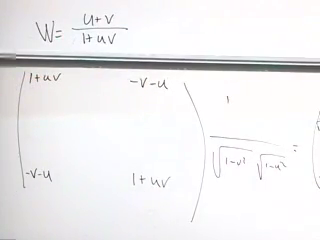
\includegraphics[width=0.82\textwidth]{lecture_05_figure_05.png}
\caption{合成ブースト行列と自然単位での速度
\(w=(u+v)/(1+uv)\)。}
\lectureframe{01:15:35}
\end{figure}

\(u\)と\(v\)がそれぞれ\(c\)に近いなら、分子は\(2c\)に近づき、分母は\(2\)に近づくので、\(w\)は\(2c\)ではなく\(c\)に近づく。より一般には、式~\eqref{eq:l5-velocity-addition}は光速以下の入力を光速以下の結果に写す。行列の積が速度限界を自動的に組み込んでいるのである。

\section{4元ベクトルと通常の速度の破綻}

4元ベクトルとは、その4つの成分が時空座標と同じように回転とローレンツブーストの下で変換するような対象である。\(V^\mu\)が4元ベクトルなら、ここでの符号の規約では
\begin{equation}
V_\mu=(-V^1,-V^2,-V^3,V^0),
\end{equation}
であり、その不変ノルムは
\begin{equation}
V_\mu V^\mu=(V^0)^2-(V^1)^2-(V^2)^2-(V^3)^2.
\end{equation}
である。2つの4元ベクトル\(V^\mu\)と\(W^\mu\)について、縮約
\begin{equation}
W_\mu V^\mu
=W^0V^0-W^1V^1-W^2V^2-W^3V^3
\end{equation}
も同様に不変である。成分は座標系の間で変化するが、縮約は変化しない。

通常の速度は3つの成分しか持たない。
\begin{equation}
\mathbf v=\left(\frac{dx}{dt},\frac{dy}{dt},\frac{dz}{dt}\right).
\end{equation}
\(dt/dt=1\)を付け加えても、それは有用な4元ベクトルにはならない。第4成分は自明なものになり、得られる対象はローレンツ変換の下で線形に変換されない。座標時間\(t\)は慣性系ごとに変わるので、\(t\)で微分すると望ましい変換則が損なわれる。

固有時間がその解決を与える。世界線に沿って
\begin{equation}
u^\mu=\frac{dX^\mu}{d\tau}.
\label{eq:l5-four-velocity}
\end{equation}
と定義する。微分\(dX^\mu\)は4元ベクトルであり、\(d\tau\)は不変量であるから、その比は4元ベクトルである。``固有''という形容詞は分母にある時計を指す。

連鎖律により、この対象は通常の速度と関係づけられる：
\begin{equation}
\frac{dx}{d\tau}=\frac{dx}{dt}\frac{dt}{d\tau},
\end{equation}
であり、\(y\)および\(z\)についても同様である。式~\eqref{eq:l5-proper-time}より
\begin{align}
\left(\frac{d\tau}{dt}\right)^2
&=1-\left(\frac{dx}{dt}\right)^2
    -\left(\frac{dy}{dt}\right)^2
    -\left(\frac{dz}{dt}\right)^2\nonumber\\
&=1-v^2
\qquad(c=1),
\end{align}
したがって
\begin{equation}
\frac{dt}{d\tau}=\gamma_v=\frac{1}{\sqrt{1-v^2}}.
\end{equation}
4つの成分は
\begin{equation}
u^i=\gamma_v v^i,
\qquad
u^0=\gamma_v
\qquad(c=1).
\label{eq:l5-four-velocity-components}
\end{equation}
である。低速では\(u^i\simeq v^i\)および\(u^0\simeq1\)である。光速に近づくと、\(\gamma_v\)は際限なく増大し、固有速度は通常の速度と著しく異なる。

\begin{figure}[H]
\centering
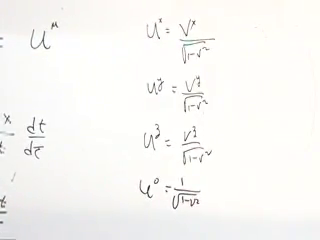
\includegraphics[width=0.82\textwidth]{lecture_05_figure_06.png}
\caption{通常の速度とローレンツ因子によって表された固有速度の4成分。}
\lectureframe{01:34:40}
\end{figure}

従来の単位を復元し、\(X^0=ct\)を用いると、ここで採用している空間成分を先に置く順序で標準的な形
\begin{equation}
U^\mu=(\gamma_v\mathbf v,\gamma_v c)
\end{equation}
が得られる。その不変ノルムは
\begin{equation}
U_\mu U^\mu=c^2.
\end{equation}
である。したがって、すべての質量を持つ粒子は、その空間速度が慣性系に依存しても、同じ不変的大きさの4元速度を持つ。

\section{世界線の接線}

式~\eqref{eq:l5-four-velocity}には、よく知られたユークリッド的な模型がある。通常の3次元空間内の曲線に沿って
\begin{equation}
ds^2=dx^2+dy^2+dz^2.
\end{equation}
である。微分変位\((dx,dy,dz)\)は曲線に沿う方向を向くが、単位ベクトルではない。弧長で割ると
\begin{equation}
\mathbf T=
\left(\frac{dx}{ds},\frac{dy}{ds},\frac{dz}{ds}\right),
\qquad
\mathbf T\cdot\mathbf T=1.
\end{equation}
が得られる。相対論的な構成は、ユークリッド的弧長の代わりに固有時間を用いた同じ考え方である。ベクトル\(u^\mu=dX^\mu/d\tau\)は世界線に接している。

\begin{figure}[H]
\centering
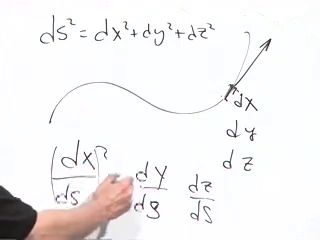
\includegraphics[width=0.82\textwidth]{lecture_05_figure_07.png}
\caption{ユークリッド的な接ベクトルの構成：微分変位を弧長要素\(ds\)で割る。固有時間は時間的向きの世界線に沿って同様の役割を果たす。}
\lectureframe{01:39:30}
\end{figure}

\begin{classroomqa}
\audiencequestion{もし\(c=1\)ならば、固有時間と固有距離は同じものか。}
\lecturerresponse{\(c=1\)と置くと時間と距離が同じ単位になるが、時空幾何学の負号が消えるわけではない。ユークリッド的な類推では、\(s\)は空間的曲線に沿って測った通常の距離である。時間的向きの世界線に沿っては、\(\tau\)は時計によって測られた経過時間である。構成は類似しているが、幾何学は異なる。}
\end{classroomqa}

もう一度微分すると固有加速度が定義される：
\begin{equation}
a^\mu=\frac{du^\mu}{d\tau}.
\end{equation}
これは、ニュートンの第2法則を相対論的にする際に\(d^2\mathbf x/dt^2\)を置き換えなければならない量である。\(u_\mu u^\mu\)は定数であるから、
\begin{equation}
\frac{d}{d\tau}(u_\mu u^\mu)=2u_\mu a^\mu=0,
\end{equation}
であり、したがって4元加速度は4元速度とミンコフスキー直交する。\editorialnote{この直交性は不変ノルムから直ちに従い、定義の次に来る数学的帰結として含められている。}

\section{4元運動量とエネルギー}

運動量を最後の例とするのは、それが衝突や崩壊において保存されるからである。粒子は固定された固有質量\(m\)を持ち、これはしばしば静止質量と呼ばれる。それは速度によって変化しない。相対論的運動量は、その固定された質量と4元速度の積である：
\begin{equation}
p^\mu=mu^\mu.
\label{eq:l5-four-momentum}
\end{equation}
\(c=1\)単位では
\begin{equation}
p^i=\gamma_v m v^i,
\qquad
p^0=\gamma_v m.
\end{equation}
である。小さな速度では\(\gamma_v\simeq1\)であるから、空間成分はニュートン的な運動量\(m\mathbf v\)に帰着する。高速ではそれらは\(m\mathbf v\)よりも急速に増大する。

時間成分はエネルギーである。従来の単位と\(X^0=ct\)を用いると
\begin{equation}
P^\mu=(\mathbf p,E/c)
=(\gamma_v m\mathbf v,\gamma_v mc),
\end{equation}
であり、したがって
\begin{equation}
E=\gamma_v mc^2
=mc^2\left(1-\frac{v^2}{c^2}\right)^{-1/2}.
\label{eq:l5-relativistic-energy}
\end{equation}
である。

通常の力学を回復するために、
\(\epsilon=v^2/c^2\ll1\)とおく。二項展開により
\begin{equation}
(1-\epsilon)^p=1-p\epsilon+O(\epsilon^2).
\end{equation}
が得られる。\(p=-1/2\)ととると、
\begin{align}
E
&=mc^2\left(1-\frac{v^2}{c^2}\right)^{-1/2}\nonumber\\
&=mc^2\left[1+\frac12\frac{v^2}{c^2}
  +O\!\left(\frac{v^4}{c^4}\right)\right]\nonumber\\
&=mc^2+\frac12mv^2+O\!\left(\frac{mv^4}{c^2}\right).
\label{eq:l5-energy-expansion}
\end{align}

\begin{figure}[H]
\centering
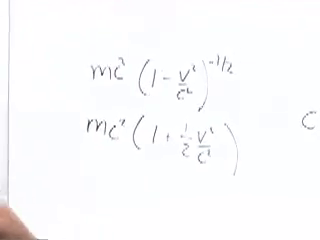
\includegraphics[width=0.82\textwidth]{lecture_05_figure_08.png}
\caption{相対論的エネルギーの低速展開。静止エネルギーとニュートン的運動エネルギーが現れる。}
\lectureframe{01:51:30}
\end{figure}

最初の項\(mc^2\)は、静止していても存在する。質量が変化しない固定された粒子の集まりを扱うニュートン的な問題では、その項は運動の前後で同じ定数を加えるだけなので、よく知られた収支に影響するのは\(\tfrac12mv^2\)だけである。相対論は、捨てられていたその定数が実はずっと物理的なエネルギーであったことを明らかにする。

したがって、エネルギーと運動量は無関係な保存則ではない。それらは1つの保存ベクトルの4つの成分である。ローレンツブーストはそれらを混合する：ある観測者がエネルギーと呼ぶものは、別の観測者の運動量に部分的に寄与し、その逆も成り立つ。それにもかかわらず、孤立系では、全4元運動量はすべての慣性系においてあらゆる衝突や崩壊の前後で同じである。

ここが相対論的力学の閾値である。次の課題は、力を固有加速度によって表すこと、および相対論的波動方程式、とりわけ電磁気学と光を支配する方程式を理解することである。
\chapter{不変な法則、四元ベクトル、場のテンソル}

まず、自然が従ってもよかったのに従っていない法則から始めよう。その失敗は、物理法則がどのように書かれるべきかを教えてくれる。同じ試練は、まず座標成分から通常のベクトルへ、次に通常のベクトルから四元ベクトルへ、最後に四元ベクトルからテンソルへと導く。最終的には、電場と磁場はもはや別々の対象ではなくなる。それらは共に、一つの反対称テンソルの6つの独立な枠を占めるのである。

特に断らない限り、\(c=1\) とする単位系を用い、時空成分を \((1,2,3,0)=(x,y,z,t)\) の順に並べ、計量の符号を \((-,-,-,+)\) とする。

\section{誤った対称性をもつ可能な法則}

空間に \(x\) 軸と \(y\) 軸を永久に固定する。次に、二つの粒子の \(x\) 座標が一致するときはいつでも相互作用すると定めよう。相互作用はそれらの運動を逆転させるかもしれないし、新しい方向へと送り出すかもしれない。その詳細な力学は問題ではない。提案された引き金は単に
\begin{equation}
  x_1-x_2=0,
\end{equation}
である。ここで添字は座標成分ではなく粒子を表す。この規則には数学的矛盾はない。問題は、何がこれを物理的にありそうにないものにするのかである。

\begin{classroomqa}
\audiencequestion{この規則は空間の一様性に反するか。}
\lecturerresponse{反しない。原点を平行移動すると両方の座標が同じ量だけ変わり、\(x_1-x_2\) は変わらない。この規則は特別な場所を指定していない。その欠陥は等方性である。すなわち、一つの特別な方向を選び出している。}
\end{classroomqa}

軸を \(90^\circ\) 回転させる。古い \(x\) 方向は今や \(y\) と呼ばれるので、同じ物理的出来事は \(y\) 座標の等しさによって記述されることになる。一般の角度では、条件は \(x\) と \(y\) の線形結合を含むことになる。したがって、法則の形は黒板がどのように向けられていたかに依存する。それは平行移動不変であるが、回転不変ではない。

通常、物理法則は直交座標において最も簡単な形で与えられる。より一般の座標を用いてもよいが、その場合には計量と公式はより簡単でなくなる。直交デカルト系の範囲内では、いかなる向きも特権的であってはならない。

修正は即座である。二次元では両方の座標が一致することを要求し、三次元では三つすべてが一致することを要求する。
\begin{equation}
  x_1=x_2,
  \qquad y_1=y_2,
  \qquad z_1=z_2.
\end{equation}
そのとき粒子は、たとえ異なる直線に沿って近づいても、同じ点に到達したときにのみ相互作用できる。

\begin{classroomqa}
\audiencequestion{\(z\) 座標と時間も一致しなければならないか。}
\lecturerresponse{三次元空間では \(z\) 座標も一致しなければならない。時間は今のところ抑えている。空間についての議論が完了し次第、復元される。}
\end{classroomqa}

\(\boldsymbol r_a\) を粒子 \(a\) の位置とする。三つの成分条件は一つのベクトル方程式になる。
\begin{equation}
  \boldsymbol r_1-\boldsymbol r_2=\boldsymbol 0.
\end{equation}
成分はある回転された系では消え、別の系では消えないかもしれない。ベクトル全体は異なる。ある系で全ての成分がゼロならば、どの回転された系でも全ての成分がゼロである。同様に、二つのベクトルがある系で等しければ、両方を変換した後でも等しいままである。

\begin{figure}[H]
\centering
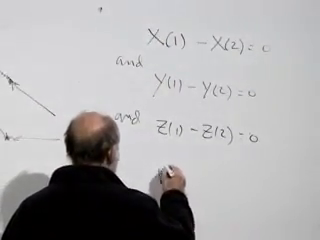
\includegraphics[width=0.78\textwidth]{lecture_06_figure_01.png}
\caption{衝突が一つの特権的な軸に沿った一致ではなく空間的な同時位置を意味するようにする三つの座標の等しさ。}
\lectureframe{00:09:00}
\end{figure}

これがベクトル方程式が有用である理由である。その成分は変化するが、対象は首尾一貫して変換する。完全な対象について書かれた法則は、座標が回転されてもその形を保つことができる。

\section{時空における同時位置}

次に、垂直な空間軸を時間で置き換える。ニュートン的な規則では、二つの運動の変化は等しい時間にのみ起こると言うかもしれない。ニュートン力学では同時性はすべての慣性観測者に共有されるので、そのような規則は可能である。特殊相対性理論では、それは特権的な系を選び出す。ある系で同時である出来事は、別の系でも同時である必要はない。

空間座標のみの等しさを要求するのも同様に良くない。時空変位は空間成分がゼロで時間成分が非ゼロでありうる。
\begin{equation}
  \Delta X^\mu=(0,0,0,\Delta t),
\end{equation}
そしてブーストは \(\Delta t\) を空間成分と混合する。不変な局所的言明は、二つの運動の変化が同じ事象で起こるということである。したがって、単純な衝突は次を要求する。
\begin{equation}
  X_1^\mu=X_2^\mu,
  \qquad\text{or}\qquad
  X_1^\mu-X_2^\mu=0.
\end{equation}
四つの座標すべてが一致する。すなわち、粒子は同じ時刻に同じ場所を占める。

衝突の例は、物理学を書くための一般的な規則を与える。すべてを一方の側に置いて完全な四元ベクトルをゼロに等しいと置くか、あるいは一つの完全な四元ベクトルを別のものに等しいと置けばよい。四元ベクトルの無関係な部分を等置することは、それ自体ではローレンツ不変な言明を与えない。

\section{ブースト、回転、行列記法}

4元ベクトルとは、時空変位と同じように変換する対象である。この定義を有用なものにするために、まず座標そのものの変換を思い出そう。\(x\)方向の速さ\(v\)のブーストに対して、
\begin{align}
  x'&=\gamma(x-vt), & y'&=y, & z'&=z,
  & t'&=\gamma(t-vx),                                      \label{eq:l6-boost}
\end{align}
ここで
\begin{equation}
  \gamma(v)=\frac{1}{\sqrt{1-v^2}}.
\end{equation}

\begin{classroomqa}
\audiencequestion{これらの式では光速が1に等しいと置かれているのか。}
\lecturerresponse{はい。単位を復元するには、\(X^0=ct\)とし、\(1-v^2\)を\(1-v^2/c^2\)に置き換え、混合した空間--時間の項に対応する\(c\)の因子を復元すればよい。}
\end{classroomqa}

\(z\)軸まわりの回転は\(x\)と\(y\)を混合し、\(z\)と\(t\)はそのままにする：
\begin{equation}
\begin{pmatrix}
  x'\\ y'\\ z'\\ t'
\end{pmatrix}
=
\begin{pmatrix}
  \cos\theta & \sin\theta & 0 & 0\\
  -\sin\theta & \cos\theta & 0 & 0\\
  0 & 0 & 1 & 0\\
  0 & 0 & 0 & 1
\end{pmatrix}
\begin{pmatrix}
  x\\ y\\ z\\ t
\end{pmatrix}.
\end{equation}
ゼロは表示する価値がある。それらは、与えられた変換後の座標にどの成分が入らないかを明示的に示している。同じ順序で、式~\eqref{eq:l6-boost}のブーストは
\begin{equation}
\begin{pmatrix}
  x'\\ y'\\ z'\\ t'
\end{pmatrix}
=
\begin{pmatrix}
  \gamma & 0 & 0 & -\gamma v\\
  0 & 1 & 0 & 0\\
  0 & 0 & 1 & 0\\
  -\gamma v & 0 & 0 & \gamma
\end{pmatrix}
\begin{pmatrix}
  x\\ y\\ z\\ t
\end{pmatrix}.
\end{equation}

回転とブーストは行列の積によって合成できる。元の\(x\)軸と一致しない方向にブーストするには、その方向を\(x\)軸へ回転し、ブーストを適用し、必要に応じて回転すればよい。これら基本行列の積は、より一般的なローレンツ変換を生成する。

\begin{classroomqa}
\audiencequestion{先に回転してからブーストするか、先にブーストしてから回転するかは重要か。}
\lecturerresponse{はい。最初の操作の後では、2番目の操作が作用する軸が変わっている。2つの行列の積は一致する必要がないので、操作の順序が重要である。}
\end{classroomqa}

これらすべての線形変換は一度に
\begin{equation}
  X'^{\mu}=\Lambda^{\mu}{}_{\nu}X^{\nu}.                  \label{eq:l6-vector-transform}
\end{equation}
と書ける。繰り返された添字\(\nu\)は\(1,2,3,0\)について和をとる。これは行列の積における通常の行ごとの列和を、添字記法で表したものにすぎない。

\begin{figure}[H]
\centering
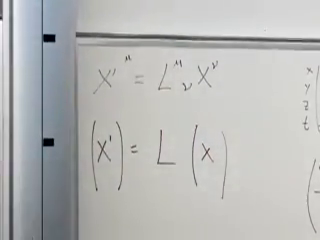
\includegraphics[width=0.78\textwidth]{lecture_06_figure_02.png}
\caption{その列ベクトル形式の冒頭より上の添字付きローレンツ変換。}
\lectureframe{00:31:55}
\end{figure}

式~\eqref{eq:l6-vector-transform}は一般の反変4元ベクトルの定義でもある。\(A^\mu\)がそのようなベクトルならば、
\begin{equation}
  A'^{\mu}=\Lambda^{\mu}{}_{\nu}A^{\nu}.
\end{equation}
その4つの成分は位置を表す必要はない。その対象を4元ベクトルにするのは、その変換則である。

\section{スカラー、計量、不変な積}

さらに4元ベクトルを使う前に、より単純なスカラーの概念に立ち返ると役に立つ。空間回転の下で、指定された点における温度はスカラーであり、指定された2点間の距離も同様である。どちらも1つの数であり、軸の向きに依存しない。センチメートルで測った距離が華氏度で測った室温に等しいという、わざとばかげた数値的主張をすることさえできる。この主張には物理的な深みはないが、両辺が回転スカラーであるため、その真偽は軸をどのように回しても依存しない。

ベクトルの成分はスカラーではない。したがって、それらをスカラーに組み合わせる体系的な方法が必要である。一般の反変4元ベクトルを
\begin{equation}
  A^\mu=(A^1,A^2,A^3,A^0).
\end{equation}
と書く。共変成分は、同じ幾何学的対象を下付き添字で表す。我々の符号では、それらはミンコフスキー計量を用いて得られ、
\begin{equation}
  A_\mu=\eta_{\mu\nu}A^\nu,
  \qquad
  \eta_{\mu\nu}=
  \begin{pmatrix}
    -1&0&0&0\\
    0&-1&0&0\\
    0&0&-1&0\\
    0&0&0&1
  \end{pmatrix},                                          \label{eq:l6-metric}
\end{equation}
したがって
\begin{equation}
  A_\mu=(-A^1,-A^2,-A^3,A^0).
\end{equation}

\begin{classroomqa}
\audiencequestion{ボード上の2つの添字と符号は矛盾しているのか。}
\lecturerresponse{はい。表示された列の空間成分には対応する負号が必要であり、添字下げの式の右辺の成分は\(\eta_{\mu\nu}\)を掛ける前に上付き添字を持つ。時間のラベルは\(4\)ではなく\(0\)である。}
\end{classroomqa}

\begin{figure}[H]
\centering
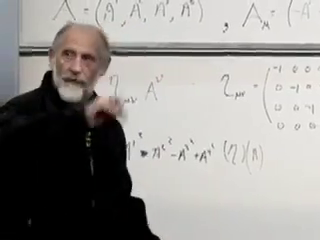
\includegraphics[width=0.8\textwidth]{lecture_06_figure_03.png}
\caption{反変成分と共変成分、計量行列、そして不変な縮約の冒頭。}
\lectureframe{00:45:00}
\end{figure}

添字下げは飾りではない。それはローレンツ不変なノルムに必要な符号をまとめる：
\begin{align}
  A_\mu A^\mu
  &=-(A^1)^2-(A^2)^2-(A^3)^2+(A^0)^2,                    \label{eq:l6-norm}\\
  X_\mu X^\mu
  &=t^2-x^2-y^2-z^2.
\end{align}
2番目の式は原点からの不変な時空間隔である。\(A^\mu\)は\(X^\mu\)と同じように変換するので、その縮約も同じ不変性を持つ。

この記法はまた、有用な勘定規則を教えてくれる。繰り返される総和添字は上付きに一度、下付きに一度現れる。例えば、
\begin{equation}
  A_\mu A^\mu
  =\eta_{\mu\nu}A^\mu A^\nu.
\end{equation}
総和される添字、すなわちダミー添字の名前は、その量を変えることなく変更してよい。

\begin{classroomqa}
\audiencequestion{これらのベクトルの一方を行、他方を列と見なすべきか、またそれらの順序は重要か。}
\lecturerresponse{現在の計算では、添字付きの量を成分と見なし、計量に縮約を行わせればよい。議論を行対列の演算子代数に変える必要はない。これらは通常の数なので、その順序は重要ではない。非可換な演算子ならばより注意が必要だが、それはここでの主題ではない。}
\end{classroomqa}

同じ構成により、異なる二つの四元ベクトルの間の内積が得られる。
\begin{equation}
  A\mathbin{\cdot}B=A_\mu B^\mu=A^\mu B_\mu.
\end{equation}
その不変性は、ローレンツ行列を陽に書くことなく従う。\(A+B\) と \(A-B\) は四元ベクトルであるから、それらのノルムの二乗はいずれも不変である：
\begin{align}
  (A+B)^2&=A^2+B^2+2A\mathbin{\cdot}B,\\
  (A-B)^2&=A^2+B^2-2A\mathbin{\cdot}B.
\end{align}
差を取ると
\begin{equation}
  (A+B)^2-(A-B)^2=4A\mathbin{\cdot}B,                    \label{eq:l6-polarization}
\end{equation}
したがって \(A\mathbin{\cdot}B\) もまた不変である。因子の4は展開から直接に従う。\editorialnote{黒板での議論がこの偏極恒等式を与える。因子を書き下すことで、口頭での相殺が曖昧でなくなる。}

\begin{figure}[H]
\centering
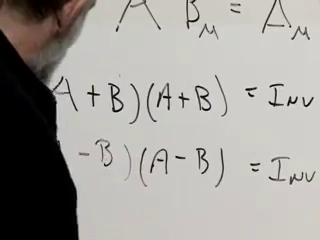
\includegraphics[width=0.8\textwidth]{lecture_06_figure_04.png}
\caption{異なる四元ベクトルの内積を分離するために用いられた二つの不変な平方。}
\lectureframe{00:52:20}
\end{figure}

不変量は物理法則の自然な構成要素である。孤立した成分と異なり、それらは座標系から座標系へと同じ値をもたらす。

\section{固有速度と四元運動量}

粒子の世界線上の隣接する二つの事象を考える。それらの隔たりは無限小四元ベクトル
\begin{equation}
  dX^\mu=(dx,dy,dz,dt).
\end{equation}
である。時間的 worldline に対して、固有時間は
\begin{equation}
  d\tau^2=dX_\mu dX^\mu
  =dt^2-dx^2-dy^2-dz^2.                                  \label{eq:l6-proper-time}
\end{equation}
により定義される。固有四元速度は
\begin{equation}
  U^\mu=\frac{dX^\mu}{d\tau}.                            \label{eq:l6-four-velocity}
\end{equation}
であり、これは選ばれた座標系の座標時間ではなく、粒子自身の固有時間に関する時空位置の変化率を測る。

\(U^\mu\) は4つの成分をもつが、独立なのは3つだけである。式~\eqref{eq:l6-proper-time} を \(d\tau^2\) で割ると
\begin{equation}
  U_\mu U^\mu=1.
\end{equation}
が得られる。したがって四元速度は単位時間的ベクトルである。未来向きの選択がその時間成分の符号を定める。

\begin{classroomqa}
\audiencequestion{\(c\) よりずっと小さい速さでは、四元速度は通常の速度に帰着するか。}
\lecturerresponse{その3つの空間成分は通常の速度に近づき、時間成分は \(c=1\) 単位で1に近づく。この関係は連鎖律を適用し \(dt/d\tau\) を計算することから従う。}
\end{classroomqa}

各空間成分について、
\begin{equation}
  U^i=\frac{dx^i}{d\tau}
     =\frac{dx^i}{dt}\frac{dt}{d\tau}
     =v^i\frac{dt}{d\tau}.
\end{equation}
式~\eqref{eq:l6-proper-time} を \(dt^2\) で割る：
\begin{equation}
  \left(\frac{d\tau}{dt}\right)^2
  =1-v_x^2-v_y^2-v_z^2
  =1-\boldsymbol v^2.
\end{equation}
したがって
\begin{equation}
  \frac{dt}{d\tau}=\frac{1}{\sqrt{1-\boldsymbol v^2}}
  =\gamma(\lvert\boldsymbol v\rvert),
\end{equation}
であり、
\begin{equation}
  U^\mu=(\gamma v_x,\gamma v_y,\gamma v_z,\gamma).
                                                                  \label{eq:l6-u-components}
\end{equation}

\begin{figure}[H]
\centering
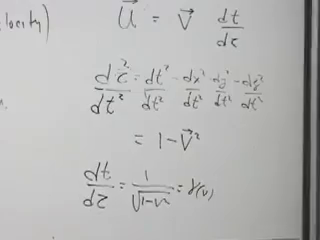
\includegraphics[width=0.8\textwidth]{lecture_06_figure_05.png}
\caption{\(dt/d\tau=\gamma\) を生み出し、固有速度を通常の速度と関係づける固有時間の計算。}
\lectureframe{01:02:00}
\end{figure}

\begin{classroomqa}
\audiencequestion{\(dx^2/dt^2\) は二階微分を意味するのか、またベクトルを二乗すると交差項が生じるべきか。}
\lecturerresponse{ここでは \((dx/dt)^2\)、すなわち一階微分の二乗を意味する。さらに \(\boldsymbol v^2\) はユークリッド内積
\(v_x^2+v_y^2+v_z^2\)
を意味し、形式和
\(v_x+v_y+v_z\)
の二乗ではない。交差項は存在しない。}
\end{classroomqa}

\begin{classroomqa}
\audiencequestion{\(\gamma(v)\) における \(v\) は二つの座標系の相対速度か、それとも粒子の速さか。}
\lecturerresponse{ここでは選ばれた座標系における粒子の速さである。関数 \(\gamma(v)=1/\sqrt{1-v^2}\) は任意の速さに対して評価できる。ブーストでは相対的な座標系の速さで評価され、四元速度では粒子の速さで評価される。}
\end{classroomqa}

\(v\ll1\) に対して \(\gamma\simeq1\) であるから、\(U^\mu\) の空間成分は \(\boldsymbol v\) に近づき、\(U^0\) は1に近づく。通常の速さが光速に近づくにつれて、\(\gamma\) および四元速度のすべての非零成分は際限なく増大する。

\begin{classroomqa}
\audiencequestion{\(U^0\) は1という数に近いのではなく、速度の単位をもつべきではないか。}
\lecturerresponse{\(c\) を1と置いたときに単位は消えた。\(X^0=ct\) では
\(U^\mu=(\gamma\boldsymbol v,\gamma c)\)
であるから、時間成分は \(c\) に近づき、\(U_\mu U^\mu=c^2\) となる。}
\end{classroomqa}

静止質量 \(m\) の粒子に対して、四元運動量を
\begin{equation}
  P^\mu=mU^\mu.
\end{equation}
により定義する。自然単位では、
\begin{equation}
  P^\mu=(\gamma m\boldsymbol v,\gamma m).
\end{equation}
である。最初の3つの成分は低速でニュートン的運動量 \(m\boldsymbol v\) に近づく。単位を復元すると
\begin{equation}
  P^\mu=(\gamma m\boldsymbol v,E/c),
  \qquad E=\gamma mc^2,
\end{equation}
が得られ、したがって
\begin{equation}
  E=mc^2+\frac{1}{2}m\boldsymbol v^2+O(mv^4/c^2).
\end{equation}
となる。時間成分は \(c=1\) 単位でのエネルギー、すなわち4つの成分すべてに運動量の単位を割り当てた場合には \(c\) で割ったエネルギーである。

\begin{classroomqa}
\audiencequestion{通常の \(\boldsymbol v\) に第4の成分を付け加えたものは、それ自体が四元ベクトルか。}
\lecturerresponse{いいえ。通常の三次元速度は四元ベクトルとして変換しない。因子 \(\gamma\) と固有時間の定義が本質的であり、四元ベクトルは \(U^\mu\) であって \(\boldsymbol v\) ではない。}
\end{classroomqa}

\section{なぜ電場と磁場は混ざり合わなければならないのか}

ここで、相対性理論からの短い休暇と呼ばれていたものに移る。アインシュタイン以前の運動方程式から出発し、それがすべての慣性系で有効であるためにはどのように再編成されなければならないかを問う。通常の加速度は通常の速度の時間微分である。その四次元的な類似物は自然に
\begin{equation}
  A^\mu=\frac{dU^\mu}{d\tau}.
\end{equation}
である。低速ではその空間成分は通常の加速度に近づく。完全な相対論的方程式は後回しにし、まず古い力の法則を調べる。

電場と磁場の中にある電荷\(q\)に対して、
\begin{equation}
  \boldsymbol F=m\boldsymbol a
  =q\left(\boldsymbol E+\boldsymbol v\times\boldsymbol B\right).
                                                                  \label{eq:l6-lorentz-force}
\end{equation}
電気の項は粒子の速度に依存しないが、磁気の項はそうではない。

\begin{figure}[H]
\centering
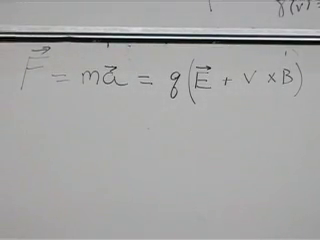
\includegraphics[width=0.8\textwidth]{lecture_06_figure_06.png}
\caption{\(\boldsymbol E\)と\(\boldsymbol B\)を組み合わせる動機となる、相対論以前の形のローレンツ力の法則。}
\lectureframe{01:18:20}
\end{figure}

ある観測者が電場を見ずに磁場と運動する電荷を見ているとしよう。その電荷は磁気的な力を受ける。しかし、その電荷の瞬間静止系では\(\boldsymbol v=0\)であるから、式~\eqref{eq:l6-lorentz-force}の磁気の項は消える。座標が変わったからといって物理的な世界線が慣性になっているわけではない。したがって、新しい系における力には電気的な寄与が含まれなければならない。より注意深く言えば、非零の四元加速度は、慣性系を変えても零に変換することはできない。ただし、三次元加速度とその成分は変換される。\editorialnote{この四元加速度についての主張は、教室での議論の不変形であり、通常の三次元加速度そのものを系に不変なものとして扱うことを避けている。}

したがって、電場と磁場は互いに変換し合わなければならない。両者を合わせると六つの成分をもつので、一つのスカラーでも一つの四元ベクトルでもない。新たな変換する対象が必要である。

\section{テンソル：各添字に一つの変換}

スカラーは階数零のテンソルと呼ばれることがある。添字をもたない。四元ベクトルは階数一のテンソルであり、四つの可能な値をもつ添字を一つもつ。最も簡単な階数二の例は積
\begin{equation}
  A^\mu B^\nu.
\end{equation}
である。各添字が四つの値をとるので、この対象は\(4^2=16\)個の成分をもち、\(4\times4\)の配列として表示できる。三つのベクトルの積
\begin{equation}
  A^\mu B^\nu C^\sigma,
\end{equation}
は\(4^3=64\)個の成分をもち、階数三のテンソルである。より高い階数もこのパターンに従う。名称よりも、その対象を定義する規則の方が重要である。

もし
\begin{equation}
  A'^{\mu}=\Lambda^\mu{}_{\nu}A^\nu,
  \qquad
  B'^{\sigma}=\Lambda^\sigma{}_{\tau}B^\tau,
\end{equation}
ならば、それらの積は
\begin{equation}
  A'^{\mu}B'^{\sigma}
  =\Lambda^\mu{}_{\nu}\Lambda^\sigma{}_{\tau}
   A^\nu B^\tau.
\end{equation}
と変換する。これにより、反変階数二テンソルの定義則が与えられる：
\begin{equation}
  T'^{\mu\sigma}
  =\Lambda^\mu{}_{\nu}\Lambda^\sigma{}_{\tau}T^{\nu\tau}.
                                                                  \label{eq:l6-tensor-transform}
\end{equation}
各添字に対して一つのローレンツ行列がある。繰り返された\(\nu\)と\(\tau\)は和をとられ、開いた\(\mu\)と\(\sigma\)はプライム系で計算される成分を表す。

\begin{figure}[H]
\centering
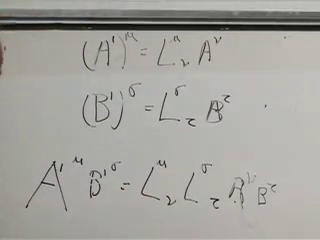
\includegraphics[width=0.82\textwidth]{lecture_06_figure_07.png}
\caption{二つのベクトルの変換と、それから得られる階数二テンソルの二行列変換則。}
\lectureframe{01:27:15}
\end{figure}

テンソルはベクトルの単一の積である必要はない。\(A^\mu B^\nu\)も\(A^\nu B^\mu\)もテンソル変換則を満たし、それらの和や
\begin{equation}
  A^\mu B^\nu+C^\mu D^\nu.
\end{equation}
のような任意の和も同様である。定義となるのは変換則であり、特定の因数分解ではない。階数三のテンソルは三つ目のローレンツ行列を獲得し、以下同様である。

\section{対称テンソルと反対称テンソル}

階数二のテンソルのうち二つのクラスが特に有用である。対称テンソルは
\begin{equation}
  T^{\mu\nu}=T^{\nu\mu},
\end{equation}
を満たすので、対角線を挟んで反射した成分は一致する。四つの対角成分と対角線の片側にある六つの成分が残りを決定し、\begin{equation}
  4+6=10
\end{equation}
個の独立成分を与える。

反対称テンソルは
\begin{equation}
  T^{\mu\nu}=-T^{\nu\mu}.                                \label{eq:l6-antisymmetry}
\end{equation}
を満たす。式~\eqref{eq:l6-antisymmetry}で\(\mu=\nu\)と置くと
\(T^{\mu\mu}=-T^{\mu\mu}\)となるので、すべての対角成分は消える。一方の三角形の半分にある六つの成分が、符号を変えることでもう六つを決定する。したがって、独立成分はちょうど六つである。

\begin{figure}[H]
\centering
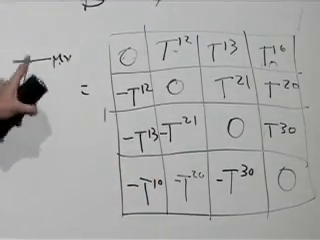
\includegraphics[width=0.82\textwidth]{lecture_06_figure_08.png}
\caption{完成した反対称\(4\times4\)配列：対角線上は零で、対角線を挟んで符号が反対。}
\lectureframe{01:34:25}
\end{figure}

この数が手がかりである。三つの電場成分と三つの磁場成分は、一つの反対称階数二テンソルに収めることができる。

\section{電磁場テンソル}

時空のラベルが\((1,2,3,0)=(x,y,z,t)\)の順で行と列に並ぶとしよう。黒板に書かれた配置は
\begin{equation}
  F_{\mu\nu}=
  \begin{pmatrix}
    0    & -B_3 & B_2  & E_1\\
    B_3  & 0    & -B_1 & E_2\\
    -B_2 & B_1  & 0    & E_3\\
    -E_1 & -E_2 & -E_3 & 0
  \end{pmatrix}.                                         \label{eq:l6-field-tensor}
\end{equation}
である。純粋に空間的な位置には磁場が入り、一つの空間添字と一つの時間添字をもつ位置には電場が入る。反対称性により、上三角成分が分かれば下三角成分が与えられる。

\begin{classroomqa}
\audiencequestion{磁気の成分はすべて負であり、ラベルは\(x,y,z\)に対応するのか。}
\lecturerresponse{上側の空間三角形における符号は示されたように交互になる：\(-B_3,+B_2,-B_1\)。ラベル\(1,2,3\)は\(x,y,z\)に対応し、一方\(0\)は時間を表す。対角線を挟んだ反射はすべての符号を逆にする。}
\end{classroomqa}

\begin{figure}[H]
\centering
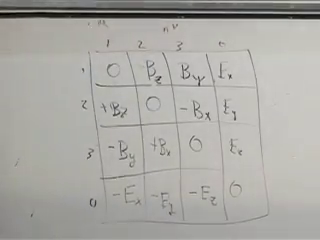
\includegraphics[width=0.82\textwidth]{lecture_06_figure_09.png}
\caption{講義の空間優先の成分順序における、完成した電磁場テンソル。}
\lectureframe{01:41:05}
\end{figure}

この記法は慣例的に\(F_{\mu\nu}\)であり、一般的な\(T_{\mu\nu}\)ではない。講師は、この文字はFaradayを指すのではないかと推測しつつも、この記法の歴史については知らないと明言している。ここで重要なのは、この文字についてのその推測ではなく、その反対称性と6つの場の成分である。

\begin{classroomqa}
\audiencequestion{各行列成分は、示された座標平面における場の強さを表しているのか。}
\lecturerresponse{それは電磁場テンソルの成分である。時間を含む成分は電場成分であり、空間--空間の成分は磁場成分を表す。}
\end{classroomqa}

時間指数をもつ行と列を切り分ける。残る\(3\times3\)の反対称ブロックが磁場である。その独立な成分は巡回的に覚えられる：
\begin{equation}
  F_{12}=-B_3,
  \qquad F_{23}=-B_1,
  \qquad F_{31}=-B_2.                                   \label{eq:l6-magnetic-cycle}
\end{equation}
最初の関係から出発し、すべてのラベルを\(1\to2\to3\to1\)に沿って進める。等価的には、
\begin{equation}
  F_{ij}=-\epsilon_{ijk}B_k,
\end{equation}
ただし\(\epsilon_{123}=+1\)とする。\editorialnote{Levi--Civitaの公式は、黒板で明示的に展開された巡回規則の簡潔な標準形である。}

\begin{figure}[H]
\centering
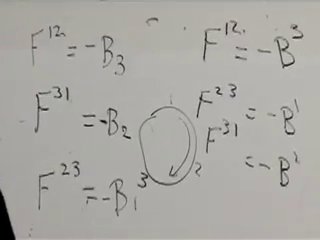
\includegraphics[width=0.82\textwidth]{lecture_06_figure_10.png}
\caption{反対称テンソルにおいて磁場を表す巡回的な空間成分。}
\lectureframe{01:46:20}
\end{figure}

電場の同定はより直接的である：
\begin{equation}
  E_1=F_{10},
  \qquad E_2=F_{20},
  \qquad E_3=F_{30}.
\end{equation}

したがって磁場には2つの有用な同一視がある。3次元空間内では、3成分の軸性ベクトルを\(3\times3\)の反対称テンソルと対応させることができる。しかし時空では、それは6成分テンソル\(F_{\mu\nu}\)の空間部分にすぎない。この対応は3次元に特有である：反対称な\(4\times4\)テンソルは6つの独立な成分をもち、4元ベクトルと同一視することはできない。\editorialnote{固有回転の下で磁場はベクトルとして振る舞うが、反射の下ではより正確には軸性ベクトル、すなわち擬ベクトルである。}

この構成の目的は、成分を数えること自体ではない。\(F_{\mu\nu}\)がテンソルとして変換するため、ローレンツブーストは自動的にその電場成分と磁場成分を混合する。次の講義では、これを4元速度および4元加速度と組み合わせて、式~\eqref{eq:l6-lorentz-force}を共変な運動方程式に置き換えることができる。

\section{EinsteinとMinkowskiに関する質問}

最後の数分は、形式論からそれが歴史的にどのように生じたかに移る。答えは確定した歴史ではなく回想として述べられ、その留保はこのやり取りの一部である。

\begin{classroomqa}
\audiencequestion{Einsteinは概念的根拠からローレンツ不変な定式化を求めていたのか、それとも特定の観測に突き動かされていたのか。}
\lecturerresponse{自然法則はすべての慣性系で同じ形をとるべきであるという原理が、彼の推論の中心にあった。光に関する実験的証拠や、エーテルを通る運動が検出されなかったこともあったが、講師は、Einsteinがどの結果を知っていたのか、あるいはそれらがどれほど強く彼に影響したのかについては明示的に不確かであると述べている。概念的圧力は、Maxwell方程式とローレンツ力が相対性原理に従うべきであり、それには電場、磁場、速度成分がともに変換することが要求されるという点にあった。}
\end{classroomqa}

Einsteinの1905年の発表は、ここで用いられている簡潔な4元ベクトル記法を使っていなかった。それは成分ごとに進められ、必要な\(\gamma\)の因子と速度が明示的に書かれていた。その後Minkowskiが、同じ構造を4次元時空として幾何学的に整理した。

\begin{classroomqa}
\audiencequestion{EinsteinはMinkowskiの時空定式化に抵抗したのか、またMinkowskiはどれほど早くそれを導入したのか。}
\lecturerresponse{授業で述べられた回想によれば、Einsteinは当初4次元幾何学的言語を歓迎しなかったが、その価値をすぐに取り入れた。時期は、1905年の論文のおよそ2年後、おそらく1907年ごろと暫定的に示され、話し手は、歴史を確定しているのではなく回想しているのだと強調する。}
\end{classroomqa}

\begin{classroomqa}
\audiencequestion{Minkowskiは数学者だったのか物理学者だったのか、他に何に貢献したのか、またLorentzやFitzGeraldの影響を受けたのか。}
\lecturerresponse{確信をもった答えは主張されない。数学者と物理学者の区別は追及されず、Minkowskiの他の仕事についての広い発言は聴衆からの訂正によって中断され、影響の可能性のある筋道は明示的に不確かなままにされる。この議論にとって確かな点は、Minkowskiが相対性理論を4次元幾何学的記法で決定的に整理したことである。}
\end{classroomqa}

\begin{classroomqa}
\audiencequestion{\(\boldsymbol E\)と\(\boldsymbol B\)を混合する変換は、すでにアインシュタインの1905年の仕事に存在していたのであろうか。}
\lecturerresponse{はい、しかし一つの場のテンソル方程式としてではなく、成分ごとに書かれていた。授業で行った比較はマクスウェルの成分方程式との比較である。内容は、その共通構造を明らかにする簡潔な記法より前に存在しうる。ミンコフスキーの貢献は、その構造を時空の言葉で体系的にしたことであった。}
\end{classroomqa}

これで、我々が出発点とした数学的な論点に戻る。成分は計算には不可欠であるが、それらの成分が一つの変換する対象の部分であると認識されるとき、法則は理解可能になる。次の課題は、\(F_{\mu\nu}\)を用いて、荷電粒子の運動方程式を、すべての慣性系で同じ形になるように書くことである。

\chapter{荷電粒子、場の変換、相対論的波動}

前回、相対性原理を課したとき、荷電粒子が電場と磁場の中でどのように運動するかを問い始めた。よく知られたローレンツ力の法則にはすでに手がかりが含まれている。その磁気的な項は粒子の速度に依存するので、異なる観測者が何が電場で何が磁場であるかについて別々に一致することはできない。我々の課題は、場と粒子の速度が座標系ごとに変わるにもかかわらず、すべての慣性観測者が同じ方程式を用いるようにこの法則を定式化することである。

特に断らない限り、\(c=1\) と計量の符号 \((-,-,-,+)\) をとる単位系を用いる。時空の成分は三つの空間成分を先にして並べる：
\begin{equation}
  \mu=(1,2,3,0)=(x,y,z,t).
\end{equation}
ラテン添字 \(m,n\) は三つの空間方向のみを走る。

\section{ニュートンの力の法則から何が生き残るか}

ニュートン力学では、
\begin{equation}
  \boldsymbol F=m\boldsymbol a
\end{equation}
はガリレイ的観測者が加速度について一致するため、すべての慣性系で同じ形をとる。彼らはまた粒子に同じ質量と同じ力を割り当てる。運動学が変われば、力と通常の加速度の間のこの特定の関係がそのまま生き残ると期待する理由はない。

電磁気学と重力はすでに、相対論的拡張が互いに似ている必要はないことを警告している。クーロンの法則とニュートンの重力の法則はどちらも逆二乗の法則であるが、重力は時空の幾何学に深い変更を加えなければ特殊相対性理論に自然に組み込むことができない。電磁気学は組み込むことができる。実際、磁気はそれ自体が相対論的効果である。\(c\) の因子を復元すると、磁気力は速度を \(c\) で割った因子を伴い、形式的な極限 \(c\to\infty\) で消える。

ニュートンの法則の耐久性のある部分は、力が運動量の変化率であるという主張である。静止質量が一定の場合、
\begin{equation}
  \boldsymbol F
  =m\frac{d\boldsymbol v}{dt}
  =\frac{d}{dt}(m\boldsymbol v)
  =\frac{d\boldsymbol p}{dt}.
\end{equation}
相対性理論は運動量と速度の関係を変えるが、この方程式の整理の仕方は保存する。

\begin{figure}[H]
\centering
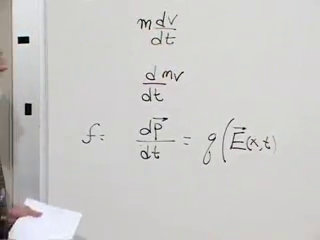
\includegraphics[width=0.64\textwidth]{lecture_07_figure_01.png}
\caption{ローレンツの法則の電気的な部分が黒板に書かれている間に、力を \(d\boldsymbol p/dt\) として書き直したもの。}
\lectureframe{00:08:20}
\end{figure}

単位 \(c=1\) では、相対論以前のローレンツ力の法則は
\begin{equation}
  \frac{d\boldsymbol p}{dt}
  =q\bigl(\boldsymbol E+\boldsymbol v\times\boldsymbol B\bigr).
  \label{eq:lorentz-three}
\end{equation}
である。両方の場は位置と時間に依存してよい。非相対論的極限は今や \(v\ll 1\) の極限であり、数値定数 \(c=1\) が何らかの形で変化する極限ではない。\eqref{eq:lorentz-three} の電気的な項はすでに通常のベクトルである。磁気的な項を時空に持ち込める形で理解するには、外積をもう一度見なければならない。

\section{反対称テンソルとしての外積}

二つの三次元ベクトル \(\boldsymbol A\) と \(\boldsymbol B\) をとる。それらの外積
\begin{equation}
  T_{mn}=A_mB_n
\end{equation}
は九つの成分をもつ二階のテンソルである。一般には対称性をもたない。反対称化すると
\begin{equation}
  K_{mn}=A_mB_n-A_nB_m,
  \qquad K_{mn}=-K_{nm}.
  \label{eq:antisym-product}
\end{equation}
が得られる。対角成分は消え、対角より下の各成分はそれに対応する上の成分によって定まる。したがって \(3\times3\) の反対称テンソルは三つの独立な成分しかもたない。

この数え上げは示唆的であるが、それだけでは十分ではない。三つの量が自動的にベクトルとして変換するわけではない。しかし三次元では、\eqref{eq:antisym-product} の三つの独立な成分を外積
\(\boldsymbol C=\boldsymbol A\times\boldsymbol B\) の成分と同一視することができる。黒板ではまず \(C_2\) を右上の位置に暫定的に置く：

\begin{figure}[H]
\centering
\includegraphics[width=0.75\textwidth]{lecture_07_figure_02.png}
\caption{その三つの独立な成分が \(\boldsymbol C\) の成分と対応づけられている間の反対称積。ここでは右上のラベルはまだ暫定的である。}
\lectureframe{00:17:33}
\end{figure}

\(1\to2\to3\to1\) を巡回させると成分の公式
\begin{align}
  C_3 &= A_1B_2-A_2B_1, \\
  C_1 &= A_2B_3-A_3B_2, \\
  C_2 &= A_3B_1-A_1B_3.
  \label{eq:cross-components}
\end{align}
が得られる。最後の行は、右上の成分が \(C_2\) ではなく \(-C_2\) であることを示している。この修正は隠すべき細部ではなく、議論の一部である。

\begin{figure}[H]
\centering
\includegraphics[width=0.62\textwidth]{lecture_07_figure_03.png}
\caption{反対称配列における暫定的な符号を確定する、完成した巡回的な成分の恒等式。}
\lectureframe{00:21:54}
\end{figure}

得られる行列は
\begin{equation}
  K_{mn}=
  \begin{pmatrix}
    0 & C_3 & -C_2 \\
    -C_3 & 0 & C_1 \\
    C_2 & -C_1 & 0
  \end{pmatrix}.
  \label{eq:cross-matrix}
\end{equation}
である。

この記法の背後には有用な幾何学がある。添字 \(1,2\) をもつ成分は自然に \(xy\) 平面に属し、それに垂直な \(z\) 軸に沿ったベクトル成分と同一視される。同じ向きづけられた対象を、平面によって記述しても、その平面に垂直な矢印によって記述してもよい。矢印による記述は三次元に特有である。より高い次元では反対称二階テンソルは依然として存在するが、もはやベクトルと同じ数の成分をもたない。したがって一般化するのは垂直な矢印ではなく、テンソルのほうである。

同値的には、向きを選んだ後で、
\begin{equation}
  C_k=\frac12\epsilon_{kmn}K_{mn}.
\end{equation}
向きを選ぶ必要があることが、右手の法則と、極性ベクトルと軸性ベクトルの間のよく知られた区別の源である。
\editorialnote{Levi--Civitaの公式と軸性ベクトルという用語は、講義で明示的に展開された平面対法線の幾何学に対する標準的な記法である。}

\section{テンソル形式の磁場}

同じ双対的な記述が磁場にも当てはまる。その反対称空間テンソルを次で定義する：
\begin{equation}
  B_{mn}=
  \begin{pmatrix}
    0 & -B_3 & B_2 \\
    B_3 & 0 & -B_1 \\
    -B_2 & B_1 & 0
  \end{pmatrix}.
  \label{eq:magnetic-tensor}
\end{equation}
\eqref{eq:cross-matrix}に対する余分な全体符号は慣習である。ひとたびそれを選べば、一貫して用いなければならない；三つのベクトル成分すべての符号を変えることは、反対の向きの慣習で同じテンソルとベクトルの同一視を記述することになる。

\begin{figure}[H]
\centering
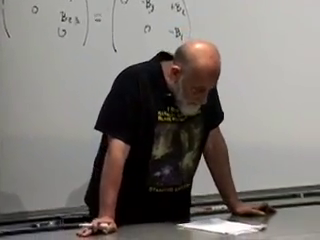
\includegraphics[width=0.72\textwidth]{lecture_07_figure_04.png}
\caption{反対称空間配列として、またその三つのベクトル成分によって書かれた磁場。}
\lectureframe{00:24:40}
\end{figure}

次に、クロス積の第3成分を取る：
\begin{align}
  (\boldsymbol v\times\boldsymbol B)_3
  &=v_1B_2-v_2B_1 \\
  &=v_1B_{13}+v_2B_{23}+v_3B_{33}.
\end{align}
最後の項は\(B_{33}=0\)であるため加えることができる。自由成分を巡回させると、次の簡潔な規則が得られる：
\begin{equation}
  (\boldsymbol v\times\boldsymbol B)_m=v_nB_{nm},
  \label{eq:cross-contraction}
\end{equation}
ここで、繰り返される添字\(n\)は和を取る。したがって、磁気力は
\begin{equation}
  F_m^{(B)}=qv_nB_{nm}.
\end{equation}

\begin{figure}[H]
\centering
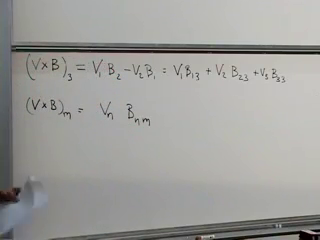
\includegraphics[width=0.78\textwidth]{lecture_07_figure_05.png}
\caption{\(\boldsymbol v\times\boldsymbol B\)の第3成分と、\(B_{nm}\)との縮約としてのその一般式。}
\lectureframe{00:28:30}
\end{figure}

\begin{classroomqa}
\audiencequestion{自由添字\(m\)は力の別個の磁気成分を表すのか？}
\lecturerresponse{いいえ。それは、計算されている力の空間成分を表す。電場は現在の議論のために単にゼロに設定されており、ここでのすべての添字は三つの空間方向にのみ走る。}
\end{classroomqa}

テンソル記法は、磁場の仕事をしない性質をほとんど自動的にする。速度の二乗を微分する：
\begin{align}
  \frac{d}{dt}(v_mv_m)
  &=2\dot v_m v_m \\
  &\propto 2(\boldsymbol v\times\boldsymbol B)_m v_m \\
  &=2v_nB_{nm}v_m.
  \label{eq:speed-derivative}
\end{align}
\(m=n\)を含む項は、\(B_{nm}\)の対角成分がゼロであるため消える。すべての非対角項には、\(m\)と\(n\)を入れ替えた相棒があり、\(v_nv_m\)は対称である一方で\(B_{nm}\)は反対称であるため、二つは相殺する。したがって
\begin{equation}
  \frac{d}{dt}(v_mv_m)=0.
\end{equation}
純粋な磁気力は、速度や運動エネルギーを変えずに軌道を曲げる。

\begin{figure}[H]
\centering
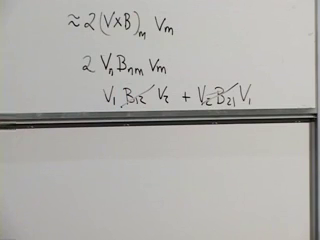
\includegraphics[width=0.68\textwidth]{lecture_07_figure_06.png}
\caption{\(v_nB_{nm}v_m\)の対になった項は、磁気テンソルが添字を入れ替えると符号を変えるため相殺する。}
\lectureframe{00:35:40}
\end{figure}

この証明は、クロス積がその最初の因子に垂直であると言うよりも意図的に手が込んでいる。後者の言明は三次元ベクトル表現に特有である。対称な対と反対称テンソルの縮約が、四次元でも生き残る議論である。

\begin{classroomqa}
\audiencequestion{速度が一定に保たれるためには、磁場は時間に依存してはならないのか？}
\lecturerresponse{上記の代数は場を微分することはなく、\(\partial_t\boldsymbol B=0\)を必要としない。磁気項だけでも依然として仕事をしない。しかし、電気力学では、変化する磁場が電場を生み、その電場が粒子の速度を変えうる。}
\end{classroomqa}

\section{なぜ電場と磁場は混ざり合わなければならないのか}

\(\boldsymbol E\)と\(\boldsymbol B\)の混合は、四次元計算の前に見ることができる。通常のニュートン的な加速度についての言明が十分であるような遅い運動を考える。磁場が\(y\)軸に沿っており、荷電粒子が\(x\)軸に沿って運動するとする。磁気力は\(z\)軸に沿って向く：
\begin{equation}
  \boldsymbol F=q\boldsymbol v\times\boldsymbol B.
\end{equation}

\begin{figure}[H]
\centering
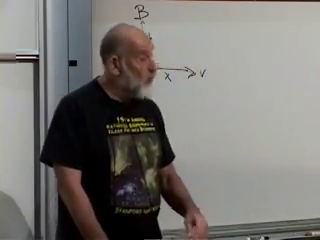
\includegraphics[width=0.62\textwidth]{lecture_07_figure_07.png}
\caption{磁場を横切って運動する粒子のための板書スケッチ；三つの方向は実験室と共動の記述を比較するために用いられる。}
\lectureframe{00:42:20}
\end{figure}

この幾何学は教室の遠近法なしで描き直すことができる：
\begin{figure}[H]
\centering
\begin{tikzpicture}[scale=1.05,>=Stealth]
  \draw[->] (0,0) -- (3.8,0) node[right] {\(x\)};
  \draw[->] (0,0) -- (-1.9,2.4) node[above left] {\(y\)};
  \draw[->] (0,0) -- (0,3.1) node[above] {\(z\)};
  \draw[->,very thick] (0,0) -- (2.7,0)
    node[midway,below] {\(\boldsymbol v\)};
  \draw[->,very thick] (0,0) -- (-1.35,1.7)
    node[midway,above left] {\(\boldsymbol B\)};
  \draw[->,very thick] (0,0) -- (0,2.35)
    node[midway,right] {\(\boldsymbol F,\ \boldsymbol E'\)};
\end{tikzpicture}
\caption{実験室では\(z\)方向の力は磁気的である；瞬間的な共動系では同じ力は電気的でなければならない。}
\end{figure}

次に、その瞬間に粒子とともに運動する観測者を導入する。新しい系での粒子の速度はゼロであるため、磁気項\(q\boldsymbol v'\times\boldsymbol B'\)は消える。しかし、遅い運動の極限では、両方の観測者が粒子が\(z\)加速度を持つことに同意しなければならない。ローレンツ力の法則が両方の系で同じ形を持つならば、共動観測者は力を\(z\)に沿った電場\(\boldsymbol E'\)に帰さなければならない。したがって、実験室で純粋に磁気的であった場は、運動系では純粋に磁気的ではない。

これが、両方の場を成分に含む単一の対象を求めるべき物理的な理由である。座標系の変更は、\(\boldsymbol E\) をそれ自身の3つの成分の間で回転させ、\(\boldsymbol B\) をそれ自身の3つの成分の間で回転させるだけではなく、2つの組を混合する。

\section{電磁場テンソル}

電場と磁場を合わせると6つの成分をもつ。4次元反対称テンソルもまた6つの独立な成分をもつ。なぜなら
\begin{equation}
  \frac{4(4-1)}{2}=6.
\end{equation}
これは、反対称テンソルが文字通り発明できる唯一の6つの量の集まりであることを意味しない。6つのスカラー、あるいはベクトルと2つのスカラーもまた6つの数を含むであろう。それは、その成分が必要とされる仕方で混合しうる自然な幾何学的対象である。

板書の規約を明示するために、反変テンソルを空間優先の順序 \((1,2,3,0)\) で表示する：
\begin{equation}
  F^{\mu\nu}=
  \begin{pmatrix}
    0 & -B_3 & B_2 & E_1 \\
    B_3 & 0 & -B_1 & E_2 \\
    -B_2 & B_1 & 0 & E_3 \\
    -E_1 & -E_2 & -E_3 & 0
  \end{pmatrix}.
  \label{eq:l07-field-tensor}
\end{equation}
左上の \(3\times3\) ブロックはまさに磁気テンソル \eqref{eq:magnetic-tensor} である。1つの空間指数と1つの時間指数をもつ成分は電場を含む。反対称性が残りの成分を与える。

\begin{figure}[H]
\centering
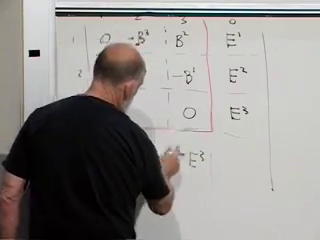
\includegraphics[width=0.72\textwidth]{lecture_07_figure_08.png}
\caption{磁気的な空間ブロックと電気的な時間-空間列が4次元場テンソルへと組み立てられる。}
\lectureframe{00:46:35}
\end{figure}

\begin{classroomqa}
\audiencequestion{これらの場の成分はいつ上付き指数をもつべきで、いつ下付き指数をもつべきか。}
\lecturerresponse{3つの空間ラベルだけについては、板書ではなじみ深いマクスウェル--ファラデー場を同定する際にその区別を省略することがある。共変的な計算ではその区別を復元しなければならない。空間指数を上げたり下げたりすることは、選ばれた計量規約において符号を変える。}
\end{classroomqa}

不変なのは、板書上の特定の符号の配置ではなく、反対称時空テンソルと、整合した計量および指数規約の組み合わせである。表記 \(F\) はファラデーを連想させるかもしれないが、講義はその歴史的帰属を自信をもって主張しているわけではない。アインシュタインは 1905 年に電場と磁場の成分の変換を導いた。コンパクトな4次元テンソル言語は、ミンコフスキーに結びつけられる後期の時空定式化とともに現れた。

\section{4元速度と4元力}

方程式の粒子側も共変的にしなければならない。固有時 \(\tau\) は不変であるから、位置4元ベクトルをそれで微分すると別の4元ベクトルが得られる：
\begin{equation}
  u^\mu=\frac{dx^\mu}{d\tau}
  =\gamma(v_x,v_y,v_z,1),
  \qquad
  \gamma=\frac{1}{\sqrt{1-v^2}}.
  \label{eq:four-velocity}
\end{equation}
最後の成分は \(dt/d\tau=\gamma\) から従う。4元運動量は
\begin{equation}
  p^\mu=mu^\mu,
\end{equation}
であり、その空間部分は相対論的運動量
\(\boldsymbol p=m\gamma\boldsymbol v\)
である。

\begin{figure}[H]
\centering
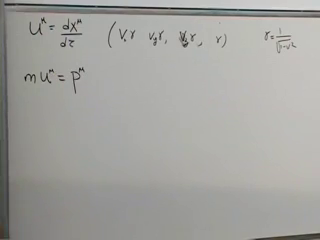
\includegraphics[width=0.75\textwidth]{lecture_07_figure_09.png}
\caption{4元速度、その成分、ローレンツ因子、および4元運動量。}
\lectureframe{00:50:30}
\end{figure}

\(p^\mu\) は4元ベクトルであり \(\tau\) はスカラーであるから、自然な相対論的左辺は
\begin{equation}
  f^\mu\equiv\frac{dp^\mu}{d\tau}.
  \label{eq:four-force-def}
\end{equation}
である。4元力は任意に選ぶことはできない。4元速度は固定されたノルムをもち、
\begin{equation}
  u_\mu u^\mu=1.
\end{equation}
世界線に沿って微分すると
\begin{align}
  0
  &=\frac{d}{d\tau}(u_\mu u^\mu) \\
  &=\frac{du_\mu}{d\tau}u^\mu
    +u_\mu\frac{du^\mu}{d\tau} \\
  &=2u_\mu\frac{du^\mu}{d\tau}.
\end{align}
が得られる。質量が一定の場合、これは
\begin{equation}
  f^\mu u_\mu=0.
  \label{eq:force-orthogonal}
\end{equation}
を意味する。したがって4元力は4元速度にミンコフスキー直交する。これは \(u^\mu\) の規格化から従う純粋に運動学的な制約であり、電磁気学に特有の性質ではない。

\begin{figure}[H]
\centering
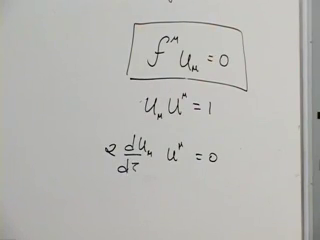
\includegraphics[width=0.64\textwidth]{lecture_07_figure_10.png}
\caption{4元速度の単位ノルムと、それから従う4元力と4元速度の直交性。}
\lectureframe{00:56:50}
\end{figure}

3次元の磁気的計算はすでに \eqref{eq:force-orthogonal} を満たすための仕掛けを与えている。反対称テンソルを速度の1つのコピーと縮約する：
\begin{equation}
  \boxed{
  \frac{dp^\mu}{d\tau}=qF^{\mu\nu}u_\nu.}
  \label{eq:covariant-lorentz}
\end{equation}
実際、
\begin{equation}
  f^\mu u_\mu
  =qF^{\mu\nu}u_\nu u_\mu=0,
\end{equation}
なぜなら \(F^{\mu\nu}\) は反対称であり、\(u_\nu u_\mu\) は対称だからである。これは考えうる唯一の相対論的力の法則ではないが、電磁場と速度の両方について線形な最も単純なものである。

\begin{figure}[H]
\centering
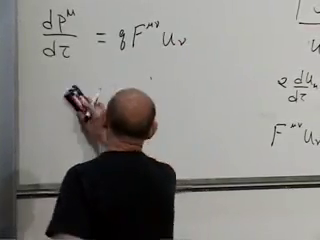
\includegraphics[width=0.72\textwidth]{lecture_07_figure_11.png}
\caption{左辺に共変的なローレンツ力方程式、右辺に第2の4元速度との消える縮約。}
\lectureframe{01:00:00}
\end{figure}

\section{通常のローレンツ力の回復}

共変的に見える方程式は、なお既知の力の法則を再現しなければならない。冒頭で述べた計量規約のもとで、
\begin{equation}
  u_\mu=\gamma(-v_x,-v_y,-v_z,1).
\end{equation}
\(x\) 成分については、\eqref{eq:l07-field-tensor} と
\eqref{eq:covariant-lorentz} から
\begin{align}
  \frac{dp^1}{d\tau}
  &=q\bigl(F^{12}u_2+F^{13}u_3+F^{10}u_0\bigr) \\
  &=q\gamma\bigl(B_3v_y-B_2v_z+E_1\bigr) \\
  &=q\gamma\bigl[\boldsymbol E+\boldsymbol v\times
    \boldsymbol B\bigr]_x.
  \label{eq:x-force}
\end{align}
が得られる。他の空間成分は指数を巡回させることで従う。

\begin{classroomqa}
\audiencequestion{成分展開における \(qE_x\) の項はどこにあるのか。}
\lecturerresponse{それは \(qF^{10}u_0\) の項である。1つの空間指数と1つの時間指数をもつ場テンソルの成分は電場の成分であり、\(u_0=\gamma\) である。}
\end{classroomqa}

右辺の因子 \(\gamma\) は余分な力ではない。
\begin{equation}
  \frac{dp^i}{d\tau}=\frac{dt}{d\tau}\frac{dp^i}{dt}
  =\gamma\frac{dp^i}{dt},
\end{equation}
であるから、\eqref{eq:x-force} の両辺から消える。したがって正確な空間方程式は再び
\begin{equation}
  \frac{d\boldsymbol p}{dt}
  =q\bigl(\boldsymbol E+\boldsymbol v\times\boldsymbol B\bigr),
  \qquad
  \boldsymbol p=m\gamma\boldsymbol v.
  \label{eq:exact-three-force}
\end{equation}
である。なじみ深い形は生き残るが、相対論は運動量の中に隠れている。

\begin{figure}[H]
\centering
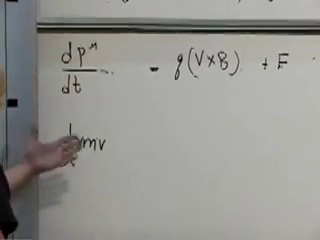
\includegraphics[width=0.75\textwidth]{lecture_07_figure_12.png}
\caption{共通の固有時因子を取り除いた後に三次元のローレンツ則が回復される。運動量は\(\gamma\)の因子を保持する。}
\lectureframe{01:06:30}
\end{figure}

時間成分は対応するエネルギーに関する命題を担い、
\begin{equation}
  \frac{dp^0}{dt}=q\boldsymbol E\cdot\boldsymbol v,
\end{equation}
したがって磁場は仕事をせず、電場は粒子のエネルギーを変化させうる。
\editorialnote{時間成分の検証は、この講義の空間的計算の直接の相棒である。これは同じ「仕事をしない」性質を四次元表記で明らかにするために含められている。}

\begin{classroomqa}
\audiencequestion{この導出は数学か物理か。}
\lecturerresponse{その両方である。テンソル代数が簡潔な形を与えるが、実質的な物理は、すべての慣性系が同じ法則に従うという原理と、運動方程式が二階であるという仮定を通じて入ってくる。二階の法則は位置と速度から未来を予測する。三階の法則ならば、加速度を追加の初期データとして必要とするだろう。自然がどちらの種類の法則を用いるかは、表記ではなく実験が教えてくれる。}
\end{classroomqa}

\section{場はどのように変換するか}

式\eqref{eq:covariant-lorentz}は、両辺が四元ベクトルであるため、どの慣性系でも同じ形をとる。場のテンソル自身は、各添字に一つずつローレンツ行列を掛けて変換する：
\begin{equation}
  F'^{\mu\nu}
  =\Lambda^\mu{}_{\rho}\Lambda^\nu{}_{\sigma}F^{\rho\sigma}.
  \label{eq:tensor-transform}
\end{equation}
黒板では、まず簡単な積\(A^\mu B^\nu\)を変換することによってこの規則を導く。ベクトルの積について規則がわかれば、線形性により任意の二階テンソルの規則が得られる。

\(1\)軸に沿ったブーストに対して、座標は次のように変換する：
\begin{align}
  x'^1&=\gamma(x^1-vx^0), &
  x'^0&=\gamma(x^0-vx^1), \\
  x'^2&=x^2, & x'^3&=x^3.
\end{align}
同じ変換を二つのテンソル添字に別々に適用する。ブーストに平行な成分について、黒板では積から始める：
\begin{align}
  (A'^0B'^1)
  =\gamma^2\bigl(
     A^0B^1-vA^0B^0-vA^1B^1+v^2A^1B^0
   \bigr).
\end{align}
各積を対応するテンソル成分に置き換え、次に反対称性\(F^{00}=F^{11}=0\)および\(F^{10}=-F^{01}\)を用いると、
\begin{equation}
  F'^{01}
  =\gamma^2(1-v^2)F^{01}
  =F^{01}.
\end{equation}
が得られる。したがって、運動に平行な電場成分は変わらない。平行な磁場成分も同様に振る舞う。

横成分は異なる。黒板で用いられたプライム系と符号の規約に従うと、
\begin{align}
  F'^{02}
  &=\gamma\bigl(F^{02}-vF^{12}\bigr), \\
  E'_2
  &=\gamma(E_2+vB_3).
  \label{eq:e-transform}
\end{align}
横電場成分は磁場成分の一部を獲得する。残りの変換則は同じ二添字規則から従い、講義の演習として残される。

\begin{figure}[H]
\centering
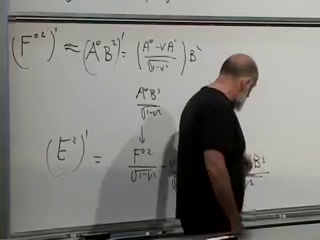
\includegraphics[width=0.76\textwidth]{lecture_07_figure_13.png}
\caption{\(E'_2\)成分が\(vB_3\)に比例する項を含むことがわかる点における横テンソル変換。}
\lectureframe{01:23:40}
\end{figure}

\eqref{eq:e-transform}における符号は、どちらの系が\(+v\)とともに動くと宣言されるか、また添字と計量の規約に依存する。その不変な内容は依存しない。横電場成分と横磁場成分は混合し、共変な力の方程式は変換後も有効である。

\begin{classroomqa}
\audiencequestion{ワイヤー中の電流について、磁場が消えるような速度で動くことはできるか。}
\lecturerresponse{伝導電子とともに動くだけでは十分でない。なぜなら、正の格子電荷が新しい系では動くからである。したがって、中性の電流を運ぶワイヤーは、単一の動く電荷の塊よりも微妙である。純粋に磁気的な場を完全に変換して消すことはできない。電場と磁場が両方存在する場合、それらの変換された部分は特別な状況で相殺しうる。一様に運動する一つの電荷については、その電荷の静止系が磁場の消える簡単な系である。}
\end{classroomqa}

正確な不変な判定は次を用いる：
\begin{equation}
  \boldsymbol B^2-\boldsymbol E^2,
  \qquad
  \boldsymbol E\cdot\boldsymbol B.
\end{equation}
\(\boldsymbol B'=0\)となる系は、\(\boldsymbol E\cdot\boldsymbol B=0\)である電場優勢の場に対してのみ存在しうる。ある系で純粋に磁気的な場は磁場優勢であり、その条件を満たすことはできない。
\editorialnote{これらの不変な判定基準は、教室での議論で到達した限定を正確に述べている。その導出は後回しにされる。}

\begin{classroomqa}
\audiencequestion{電気スカラーポテンシャルと磁気ベクトルポテンシャルは四元ベクトルをなすか。}
\lecturerresponse{はい。規約に依存する符号とともに、それらは四元ポテンシャル\(A^\mu\)に結合する。マクスウェル方程式はその対象を体系的に用いるであろう。}
\end{classroomqa}

\section{場の微分}

ここで一つの粒子の軌道を離れ、時空全体にわたる場を考える。
\begin{equation}
  \phi=\phi(x^1,x^2,x^3,x^0)
\end{equation}
をスカラー場とする。その四つの微分は四元ベクトルの共変成分をなす：
\begin{equation}
  \partial_\mu\phi
  \equiv\frac{\partial\phi}{\partial x^\mu}
  =\left(
    \frac{\partial\phi}{\partial x},
    \frac{\partial\phi}{\partial y},
    \frac{\partial\phi}{\partial z},
    \frac{\partial\phi}{\partial t}
  \right).
\end{equation}
ローレンツ座標変換に連鎖律を適用すると、この共変変換則が証明される。添字を上げると空間の符号は反転するが、時間の符号は変わらない：
\begin{equation}
  \partial^\mu\phi
  =\left(
    -\frac{\partial\phi}{\partial x},
    -\frac{\partial\phi}{\partial y},
    -\frac{\partial\phi}{\partial z},
    \frac{\partial\phi}{\partial t}
  \right).
\end{equation}

微分するごとに下付き添字が付加される。したがって
\(\partial_\nu V^\mu\) は上付き添字を1つと下付き添字を1つもつ階数2のテンソルであり、テンソルを微分すると下付き添字が1つ増えた対象が得られる。これが、好みの慣性系を選ぶことなく場の方程式を書くために必要な基本規則である。

\section{不変なスカラー波動方程式}

最も単純な波動方程式は2階の微分を含む。方程式がすべての慣性系で同じ形をもつためには、その左辺はスカラーでなければならない。微分の添字を縮約すると、一意に最も単純な選択が得られる：
\begin{equation}
  \boxed{\partial^\mu\partial_\mu\phi=0.}
  \label{eq:wave-covariant}
\end{equation}
現在の計量で成分を書き下すと、
\begin{equation}
  \frac{\partial^2\phi}{\partial t^2}
  -\frac{\partial^2\phi}{\partial x^2}
  -\frac{\partial^2\phi}{\partial y^2}
  -\frac{\partial^2\phi}{\partial z^2}=0.
  \label{eq:wave-components}
\end{equation}
\eqref{eq:wave-covariant} における縮約はローレンツ不変性を明白にする。方程式 \eqref{eq:wave-components} は同じ事柄を成分ごとに書いたものである。

\begin{figure}[H]
\centering
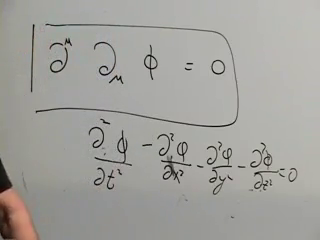
\includegraphics[width=0.75\textwidth]{lecture_07_figure_14.png}
\caption{スカラー波動方程式の縮約された微分形と、その時間マイナス空間の成分展開。}
\lectureframe{01:39:40}
\end{figure}

\begin{classroomqa}
\audiencequestion{波動方程式の右辺はゼロでなければならないのか？}
\lecturerresponse{いいえ。問題と両立する任意のスカラーでよい。\(\phi\) の定数倍や、\(\phi^2\) に比例するような非線形スカラー関数でも、共変性は保たれる。ゼロの場合が最も単純な自由波動方程式を与える。}
\end{classroomqa}

このスカラーの例の要点は準備である。マクスウェル方程式は電場と磁場をより複雑に混ぜ合わせるが、それらもまた、その添字構造からローレンツ不変性が見えるように書くことができる。それが次回に戻る問題である。

\chapter{計量、膨張、そして最初の宇宙論}

前回の講義の終わりに、われわれはローレンツ不変な波動方程式に到達し、マクスウェル方程式を時空の形で書く準備をしていた。ここで聴衆からの質問が、重力へ移る前に有用な警告を与えてくれる。すなわち、対称性だけによって物理理論のどこまでが決定されるのか、という問いである。答えは断固としている。多くを決定するが、すべてではない。ローレンツ不変性は可能な法則に対する強力なフィルターである。しかしそれは、残りの物理的仮定や実験の代わりにはならない。

\section{対称性が決定しないもの}

\begin{classroomqa}
\audiencequestion{電場と磁場がローレンツ変換の下でともに変換することが分かったなら、マクスウェル方程式は相対性理論だけから導かれるのか。}
\lecturerresponse{否である。相対性理論は方程式の形を制約するが、その構成には方程式の線形性、その導関数の低い次数、場の変換の仕方、そして実験的情報も用いられる。それらの追加の要素がなければ、多くのローレンツ共変な場の方程式が依然として可能であろう。}
\end{classroomqa}

冒頭の議論にとって、それらの追加の仮定のうち最も重要なものは線形性である。\(A(x,t)\) が線形な場の方程式の解ならば、任意の定数 \(\lambda\) に対して \(\lambda A(x,t)\) もまた解である。\(A\) と \(B\) が解ならば、
\begin{equation}
  C(x,t)=A(x,t)+B(x,t).
  \label{eq:superposition}
\end{equation}
もまた解である。これが重ね合わせの原理である。2つの源のない電磁波は互いに交差しても変化せずに出てくる。それらは物質的な物体のように直接衝突するのではない。それらは荷電物質を通じて間接的に相互作用しうる。なぜなら各々の波は電荷を動かし、動く電荷は放射するからであるが、真空の場の方程式そのものは線形である。

\begin{figure}[H]
\centering
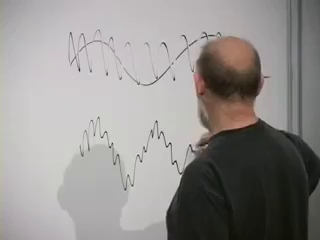
\includegraphics[width=0.64\textwidth]{lecture_08_figure_01.png}
\caption{重ね合わせの議論の際に黒板に示された2つの波のプロファイル。それらの和もまた許される源のない波である。}
\lectureframe{00:05:30}
\end{figure}

調和振動子はこの代数を透明にする。次を仮定する。
\begin{equation}
  m\ddot x=-kx.
  \label{eq:linear-oscillator}
\end{equation}
\(x_1\) と \(x_2\) が \eqref{eq:linear-oscillator} を解くならば、
\begin{equation}
  m(\ddot x_1+\ddot x_2)
  =-k(x_1+x_2),
\end{equation}
であるから、\(x_1+x_2\) は解である。しかし非線形項を加えると、
\begin{equation}
  m\ddot x=-kx+p x^2,
  \label{eq:nonlinear-oscillator}
\end{equation}
和はもはや成り立たない。
\begin{equation}
  (x_1+x_2)^2=x_1^2+x_2^2+2x_1x_2.
\end{equation}
交差項 \(2x_1x_2\) は2つの別々の方程式には対応するものがない。2つの運動は今や互いに影響を及ぼし合う。

\begin{figure}[H]
\centering
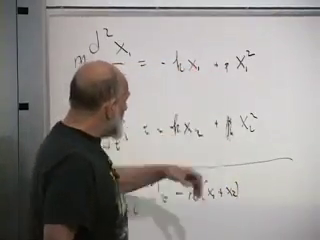
\includegraphics[width=0.73\textwidth]{lecture_08_figure_02.png}
\caption{分離した振動子の方程式を、それらの和の方程式と比較する。二次の項によって、重ね合わせを破る余分な交差項が現れる。}
\lectureframe{00:10:10}
\end{figure}

この例は、宇宙論の議論を通じて有効であり続ける方法論上の要点を確定する。対称性は、どの量が組み合わされうるか、どの方程式が許されるかを教える。力学と観測が、許された方程式のうち自然がどれを用いるかを教える。

\section{幾何学としての間隔}

ここで電磁気学を離れ、一般相対性理論と宇宙論への短い道筋に入る。出発点となる対象は、隣り合う事象の間の間隔である。ある事象を4つの座標\(x^\mu\)でラベルし、近くの事象を\(x^\mu+dx^\mu\)でラベルする。慣性系のデカルト座標において、\(c=1\)および\((+,-,-,-)\)の規約を用いると、
\begin{equation}
  d\tau^2
  =dt^2-dx^2-dy^2-dz^2
  =dx^\mu dx_\mu
  =\eta_{\mu\nu}\,dx^\mu dx^\nu.
  \label{eq:minkowski-interval}
\end{equation}
不変なのは量\(d\tau^2\)であり、座標差のどれか一つではない。ローレンツ変換は\(dt,dx,dy,dz\)を変化させるが、この二次の組み合わせは保つ。したがって特殊相対性理論は、ミンコフスキー時空の幾何学として読むことができる。

\begin{figure}[H]
\centering
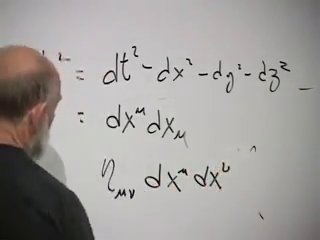
\includegraphics[width=0.72\textwidth]{lecture_08_figure_03.png}
\caption{ミンコフスキー間隔を、成分表示、縮約された添字表示、計量テンソル表示で順に書いたもの。}
\lectureframe{00:14:50}
\end{figure}

\eqref{eq:minkowski-interval} の単純さは座標に依存する。平らな平面でさえ、賢明でないラベルの付け方をすれば見慣れない係数を得る。\(x\) をセンチメートルで測り、\(y\) をメートルで測るとする。物理的な変位に対して、
\begin{equation}
  ds^2=dx^2+\left(\frac{dy}{100}\right)^2
      =dx^2+10^{-4}dy^2.
  \label{eq:mixed-units}
\end{equation}
因子 \(10^{-4}\) は曲率について何も語らない。それは単に単位間の換算を行うだけである。

\begin{figure}[H]
\centering
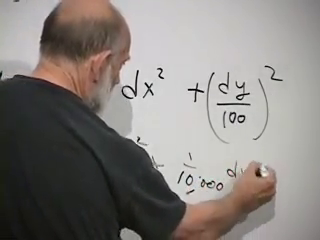
\includegraphics[width=0.59\textwidth]{lecture_08_figure_04.png}
\caption{一方の軸をセンチメートル、他方をメートルで記述した平らな平面。等しくない計量係数は曲率ではなく単位を表している。}
\lectureframe{00:20:10}
\end{figure}

斜交座標では混合項が加わる。2次元では、最も一般的な局所二次形式は
\begin{align}
  ds^2
  &=a_{11}\,dx^2+a_{12}\,dx\,dy\notag\\
  &\quad+a_{21}\,dy\,dx+a_{22}\,dy^2,
  \qquad a_{12}=a_{21}.
  \label{eq:quadratic-form}
\end{align}
と書ける。通常の微分は可換であるから、\(dx\,dy=dy\,dx\)であり、係数配列の対称部分のみが寄与する。係数をまとめて行列
\begin{equation}
  g=
  \begin{pmatrix}
    a_{11} & a_{12}\\
    a_{21} & a_{22}
  \end{pmatrix}.
  \label{eq:metric-matrix}
\end{equation}
を得る。この行列が\emph{計量}である。これは座標差を物理的な間隔へ変換する局所的な規則である。

\begin{figure}[H]
\centering
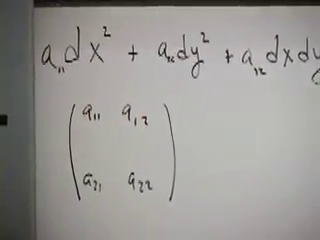
\includegraphics[width=0.71\textwidth]{lecture_08_figure_05.png}
\caption{二次微分形式と、その対称な\(2\times2\)係数行列。この行列が計量として同定される時点でのものである。}
\lectureframe{00:24:07}
\end{figure}

一様な矩形格子または斜交格子では、係数は一定になる。座標線が曲がったり、互いに密集したり、離れていったりすると、下にある面が平坦なままであっても、それらの係数は位置の関数になる。一般の時空の表記は
\begin{equation}
  ds^2=g_{\mu\nu}(x)\,dx^\mu dx^\nu.
  \label{eq:general-metric}
\end{equation}

\begin{figure}[H]
\centering
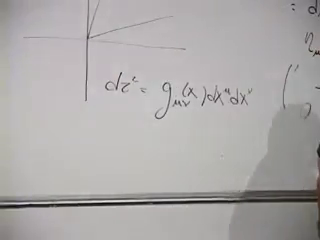
\includegraphics[width=0.66\textwidth]{lecture_08_figure_06.png}
\caption{座標格子が点ごとに変化することを許した後の、一般の位置依存計量。}
\lectureframe{00:28:10}
\end{figure}

指定された座標系で\(g_{\mu\nu}\)がわかれば、局所的な距離、時間、角度が決まり、それによって幾何が決まる。逆は一意ではない。一つの幾何には無限に多くの座標記述があり、したがって座標変換で互いに関係づけられる無限に多くの係数関数の配列がある。

\section{座標の複雑さと内在的曲率}

ここで、複雑な計量と曲がった空間を区別しなければならない。紙を引き伸ばさずに円筒に丸める。部屋の中での見え方は変わるが、紙の内部で測られるすべての距離は同じままである。紙に閉じ込められた生き物は、いかなる内在的測定によっても、その曲げを検出できない。それは外在的な曲げであり、ここで意味している曲率ではない。

半球は異なる。引き伸ばしたり、破いたり、圧縮したりせずに平らに押しつぶすことはできない。地球の平らな地図は、距離、面積、角度、またはそれらの何らかの組み合わせを歪めざるを得ない。この障害は内在的であり、周囲の次元を覗き込むことなく検出できる。

極座標は不可欠な平坦な反例を与える。平面上では、無限小の動径方向の変位の長さは\(dr\)であり、半径\(r\)における角度変位\(d\theta\)の長さは\(r\,d\theta\)である。したがって
\begin{equation}
  ds^2=dr^2+r^2d\theta^2,
  \qquad
  g_{\text{polar}}=
  \begin{pmatrix}
    1&0\\
    0&r^2
  \end{pmatrix}.
  \label{eq:polar-metric}
\end{equation}
係数\(r^2\)は平面全体で変化するが、平面は平坦である。変数変換
\begin{equation}
  x=r\cos\theta,\qquad y=r\sin\theta
\end{equation}
は一定の計量\(ds^2=dx^2+dy^2\)を返す。

\begin{figure}[H]
\centering
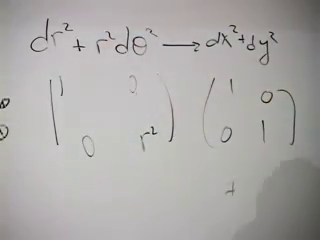
\includegraphics[width=0.70\textwidth]{lecture_08_figure_07.png}
\caption{極座標計量とそのデカルト計量への回帰。左側の位置依存行列は依然として平坦な平面を記述している。}
\lectureframe{00:39:20}
\end{figure}

\begin{classroomqa}
\audiencequestion{極座標における角度距離にはサインが含まれるべきか。}
\lecturerresponse{平面上では含まれない。そこでは弧の長さは
\(r\,d\theta\)である。サインは球面上に現れ、そこでは緯度円の半径は\(R\sin\theta\)である。}
\end{classroomqa}

半径\(R\)の球を考える。\(\theta\)を北極から測った極角、\(\phi\)を方位角とする。子午線方向の歩みの長さは\(R\,d\theta\)である。極角\(\theta\)において、緯度円の半径は\(R\sin\theta\)であるから、方位角方向の歩みの長さは
\(R\sin\theta\,d\phi\)である。局所的なピタゴラスの定理により
\begin{align}
  ds^2
  &=R^2\left(d\theta^2+\sin^2\theta\,d\phi^2\right),
  \label{eq:sphere-metric}\\
  g_{\text{sphere}}=
  &\begin{pmatrix}
    R^2&0\\
    0&R^2\sin^2\theta
  \end{pmatrix}.
\end{align}

\begin{figure}[H]
\centering
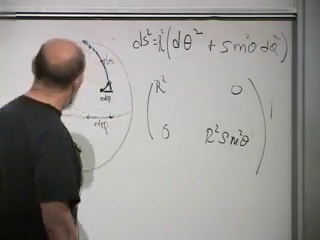
\includegraphics[width=0.72\textwidth]{lecture_08_figure_08.png}
\caption{球、その角度線素、および対応する計量行列。\(\sin^2\theta\)因子は緯度円が縮むことを記録している。}
\lectureframe{00:45:15}
\end{figure}

\begin{figure}[H]
\centering
\begin{tikzpicture}[scale=1.05]
  \draw (0,0) circle (2.1);
  \draw[dashed] (-2.1,0) arc (180:360:2.1 and 0.52);
  \draw (2.1,0) arc (0:180:2.1 and 0.52);
  \coordinate (P) at (48:2.1);
  \fill (P) circle (1.5pt);
  \draw (0,0) -- (0,2.1);
  \draw (0,0) -- (P);
  \draw (0,0.82) arc (90:48:0.82);
  \node at (0.47,1.03) {\(\theta\)};
  \draw[->] (P) -- ++(-0.34,0.36)
    node[midway,left] {\(R\,d\theta\)};
  \draw[->] (P) -- ++(0.76,0)
    node[midway,above] {\(R\sin\theta\,d\phi\)};
\end{tikzpicture}
\caption{\eqref{eq:sphere-metric}を得るために用いた局所的な微分の脚の明快な再構成。}
\end{figure}

\eqref{eq:sphere-metric}を一定のユークリッド行列に変える大域的な座標変換は存在しない。二次元の観測者はこれを内在的に発見できる。測地線から作られた十分に大きな三角形の角の和は\(180^\circ\)より大きい。したがって、有用な判定基準に到達した。係数が変化することは、それ自体では曲率を意味しない。曲率とは、考察対象の領域全体で計量を一定にする座標を見つけることへの障害である。

\section{曲がった時空から宇宙論へ}

一般相対性理論は、時空自体がこの内在的曲率を持つことを許す。位置依存の\(g_{\mu\nu}\)は、極座標の場合のように、依然として座標の産物でありうるが、真に曲がった時空では、いかなる座標変換もその変化を大域的に取り除かない。

\begin{figure}[H]
\centering
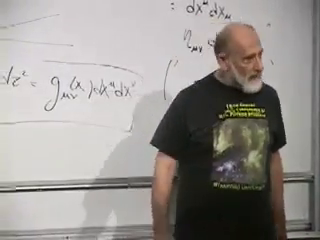
\includegraphics[width=0.70\textwidth]{lecture_08_figure_09.png}
\caption{特殊な座標の例から一般の時空線素\(ds^2=g_{\mu\nu}(x)dx^\mu dx^\nu\)への移行。}
\lectureframe{00:48:40}
\end{figure}

アインシュタイン方程式の完全な機構を試みることはしない。代わりに、宇宙論に適した幾何に注意を限定する。空間は十分に大きなスケールで一様であるとされ、一方で幾何は時間とともに変化しうる。一様とは、ある場所が別の場所から区別されないことを意味する。平坦であることを意味しない。球面上のすべての点は等価であるが、球面は曲がっている。また、あらゆるスケールで特徴がないことを意味するのでもない。

\begin{classroomqa}
\audiencequestion{銀河が集団、板、フィラメントを形成しているのに、なぜ宇宙は一様でありうるのか。}
\lecturerresponse{この主張は粗視化されたスケールに関するものである。恒星、銀河、銀河団は強く非一様である。数億光年にわたる領域を比較すると、それらの構造は一様な分布へと平均化される。宇宙原理は経験的な作業仮説であり、論理的必然ではない。宇宙背景における方向依存の差を含む、十分に大きな系統的差異があれば、それを反証しうる。}
\end{classroomqa}

この講義における第二の大規模な仮定は、空間的な平坦性である。固定された宇宙時刻において、十分に大きな三角形はユークリッド的に見える。すなわち、その角度の和は\(180^\circ\)となる。これは三次元空間の幾何学についての主張であり、まだ四次元時空の曲率についてのものではない。

\begin{classroomqa}
\audiencequestion{宇宙論的距離だけ離れた点にとって、それらの光が異なる時刻に我々に届くのだから、同時性とは何を意味するのか。}
\lecturerresponse{遠方の銀河の間に棒を置くことも、それらを瞬時に調べることもできない。我々は信号を後になって受け取り、時空模型の内部で放出事象の幾何学を再構成する。この手続きは間接的であるが、天文学における多くの幾何学的測定も同様である。平坦性とは、再構成された大きな三角形が、調査されたスケールにおいて検出可能な角度の過剰も不足も示さないことを意味する。}
\end{classroomqa}

\section{共動座標とスケール因子}

銀河の大規模な流れの上に描かれたデカルト格子を想像せよ。格子が膨張するにつれて、各銀河はその座標ラベルを保つ。そのラベルはメートル単位の距離ではなく、住所である。時間に依存する変換因子が、座標の隔たりを物理的な隔たりに変える。

\begin{figure}[H]
\centering
\begin{tikzpicture}[>=Latex,scale=0.86]
  \foreach \x in {0,0.65,1.3,1.95,2.6} {
    \draw[gray!65] (\x,0) -- (\x,2.2);
  }
  \foreach \y in {0,0.55,1.1,1.65,2.2} {
    \draw[gray!65] (0,\y) -- (2.6,\y);
  }
  \fill[blue!65!black] (0.65,0.55) circle (2pt);
  \fill[red!70!black] (1.95,1.65) circle (2pt);
  \node[below] at (1.3,-0.2) {comoving labels at \(t_1\)};
  \draw[->,very thick] (3.0,1.1) -- (4.0,1.1)
    node[midway,above] {\(a(t)\) grows};
  \foreach \x in {4.4,5.5,6.6,7.7,8.8} {
    \draw[gray!65] (\x,0) -- (\x,2.2);
  }
  \foreach \y in {0,0.55,1.1,1.65,2.2} {
    \draw[gray!65] (4.4,\y) -- (8.8,\y);
  }
  \fill[blue!65!black] (5.5,0.55) circle (2pt);
  \fill[red!70!black] (7.7,1.65) circle (2pt);
  \node[below] at (6.6,-0.2) {same labels at \(t_2\)};
\end{tikzpicture}
\caption{共動的な住所は固定されたままであり、一方で座標格子の物理的な間隔は増大する。}
\end{figure}

空間的な一様性は、与えられた時刻においてどこでも同じ変換因子を要求する。空間的な平坦性は、計量の空間部分がデカルト的であることを許す。結果として得られる線素は
\begin{equation}
  d\tau^2
  =dt^2-a^2(t)\left(dx^2+dy^2+dz^2\right).
  \label{eq:flrw-flat}
\end{equation}
である。これは共動座標における空間的に平坦で一様な宇宙論的計量である。\(x,y,z\)を無次元に選び、\(a(t)\)に長さの単位を与えてもよい。別の規約では、次元を座標に押し込み、\(a\)を無次元にすることもできる。重要なのは積だけである。

\begin{figure}[H]
\centering
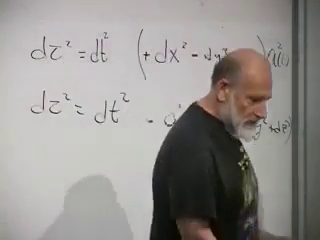
\includegraphics[width=0.76\textwidth]{lecture_08_figure_10.png}
\caption{黒板で完成された、空間的に平坦な宇宙論的計量。共通因子\(a^2(t)\)が三つの空間方向すべてに掛かっている。}
\lectureframe{01:03:15}
\end{figure}

もし\(a\)が定数であれば、\(x,y,z\)を再スケールすることによってそれを吸収でき、\eqref{eq:flrw-flat}は異なる単位での通常のミンコフスキー時空となるであろう。その時間依存性が非自明な要素である。

\begin{classroomqa}
\audiencequestion{座標格子が膨張するなら、なぜメートル棒、原子、銀河はそれとともに膨張しないのか。}
\lecturerresponse{計量は平均的な宇宙の流れを記述するものであり、すべての束縛系がそれに従うことを強制する力ではない。電磁気力がメートル棒と原子をまとめており、自己重力が銀河をまとめている。それらの束縛効果は、小さなスケールにおいて極めて弱い背景膨張を支配している。近傍の銀河はハッブル流から外れることもある。アンドロメダは天の川銀河へと引かれている。銀河の束縛に関する詳細な研究は、可視物質だけでは不十分であることを示しており、これは暗黒物質の論拠の一つである。}
\end{classroomqa}

\begin{classroomqa}
\audiencequestion{なぜスケール因子それ自体は、銀河を押し離す力ではないのか。}
\lecturerresponse{現在の規約ではそれは長さの次元をもち、力ではない。上向きに打ち出された砲弾を考えよ。一度打ち出されれば、その外向きの運動は慣性的である。重力はその運動を、速度を減らすか引き戻すことによって変える。同様に、膨張は運動の状態である。力学上の問いは、重力と他の源が\(\dot a\)と\(\ddot a\)をどのように変えるかであり、\(a\)を動かし続けるためにどのような力が必要かではない。}
\end{classroomqa}

古い予想では、引力性の重力が膨張を減速させるはずであった。この講義の時点までに、天文学的証拠は最近の膨張がむしろ加速していることを示しており、それは完全な力学が通常の引力性物質以上のものを含むことを意味する。その問題は、幾何学的な設定が確立されるまで延期する。

\section{ハッブルの法則}

固定された座標間隔が
\(\Delta x\)
である2つの共動銀河を取る。共通の宇宙時刻において、それらの物理的距離は
\begin{equation}
  D(t)=a(t)\,\Delta x.
  \label{eq:physical-distance}
\end{equation}
である。共動ラベルを固定したまま微分すると、
\begin{align}
  V(t)
    &=\dot D(t)
      =\dot a(t)\,\Delta x \nonumber\\
    &=\frac{\dot a(t)}{a(t)}D(t).
  \label{eq:hubble-derivation}
\end{align}
となる。
\begin{equation}
  H(t)=\frac{\dot a(t)}{a(t)}.
  \label{eq:hubble-parameter}
\end{equation}
と定義する。すると
\begin{equation}
  V(t)=H(t)D(t).
  \label{eq:hubble-law}
\end{equation}
となる。ある一つの宇宙時刻においては、同じ\(H(t)\)がどこでも成り立つ。そうでなければ空間は一様ではない。後退速度が距離に比例するのは、共動格子のすべての間隔が同じ割合で引き伸ばされるからである。

\begin{figure}[H]
\centering
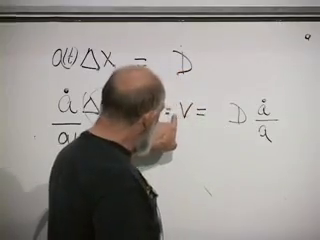
\includegraphics[width=0.73\textwidth]{lecture_08_figure_11.png}
\caption{物理的距離\(D=a\Delta x\)と、\(V=(\dot a/a)D\)に至るその時間微分。}
\lectureframe{01:16:45}
\end{figure}

\begin{classroomqa}
\audiencequestion{遠方の銀河に対して、ハッブルパラメータは現在の値で評価すべきか、それとも観測された光が放出された時点の値で評価すべきか。}
\lecturerresponse{記述されている時代の値で評価する。遠方の銀河からの光は、より早い時代の膨張の値を伝える。厳密な解析では\(H\)の時間依存性を考慮しなければならない。現在の値をどこにでも代入するのは局所近似にすぎない。}
\end{classroomqa}

\begin{classroomqa}
\audiencequestion{\(D=a\Delta x\)において単位はどこに存在するのか。}
\lecturerresponse{便利な選択は、共動ラベル\(\Delta x\)を無次元として扱い、\(a\)に長さを持たせることである。逆の記帳も可能である。いずれにせよ、\(H=\dot a/a\)は時間の逆数の次元を持つ。}
\end{classroomqa}

\section{膨張する座標における光}

光はヌル経路に従う。そのような経路に沿って固有時間間隔は消える：
\begin{equation}
  d\tau^2=0.
\end{equation}

\begin{classroomqa}
\audiencequestion{なぜ光に対して間隔はゼロなのか。}
\lecturerresponse{それが相対性理論における光線の定義的な幾何学である。すべての局所的自由落下観測者は光が\(c=1\)で進むと測定するので、局所的に\(dt^2=d\ell^2\)となり、時空間隔は消える。これは光を受け取る観測者に対して座標時間が経過しないという意味ではない。}
\end{classroomqa}

\(x\)方向のみに進む光線に対して、
\begin{equation}
  0=dt^2-a^2(t)\,dx^2.
\end{equation}
\(x\)が増加する向きに進む光線を選ぶと、
\begin{equation}
  dt=a(t)\,dx,
  \qquad
  dx=\frac{dt}{a(t)},
  \qquad
  \frac{dx}{dt}=\frac{1}{a(t)}.
  \label{eq:null-ray}
\end{equation}

\begin{figure}[H]
\centering
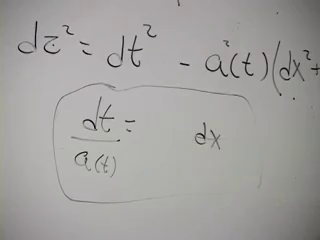
\includegraphics[width=0.64\textwidth]{lecture_08_figure_12.png}
\caption{膨張計量におけるヌル条件と、それから得られる共動光線方程式\(dx=dt/a(t)\)。}
\lectureframe{01:23:45}
\end{figure}

座標速度\(dx/dt\)はスケール因子が大きくなるにつれて減少する。これは光が局所的に遅くなるという意味ではない。1単位の共動座標距離はますます大きな物理的距離を表すので、座標速度の数値は変化するが、すべての局所測定は依然として\(c=1\)を与える。

\section{なぜ時間依存性が重要か}

中心的な幾何学の問いは今や避けられない：\(a(t)\)はどのように変化するのか。類推は、ある瞬間の位置がわかっている投射物である。その未来の軌道には運動方程式が必要である。宇宙論では、重力力学が\(a(t)\)の方程式を与えるであろう。

\begin{classroomqa}
\audiencequestion{なぜ\(a(t)\)が変化するかという問いを、たとえば電子電荷が時間とともに変化するかという同等に正当な問いよりも特権的に扱うのか。}
\lecturerresponse{論理的な階層は存在しない。電子電荷の測定された変化は極めて重要であろう。我々が\(a(t)\)に注目するのは、観測がすでに宇宙の間隔が変化することを教えているのに対し、電子電荷は一定に見えるからである。幾何学的には、一定の\(a\)は空間単位の変更によって除去でき、平坦な時空を残すであろう。時間依存の\(a\)はそのようには除去できない。}
\end{classroomqa}

遠方の後退を測定する前に、何が測定されているかを言うためにこの幾何学的枠組みが必要である。最も粗いレベルでは、既知の光度の光源は、その光がより大きな面積に広がるため距離とともに暗く見える。一方、既知の原子スペクトル線の変位は赤方偏移を与え、したがって後退の指標を与える。ハッブルは距離推定と赤方偏移を組み合わせて比例関係
\eqref{eq:hubble-law}
を明らかにしたが、係数の初期の数値はかなり誤っていた。現代の距離はしごと相対論的光伝播計算はずっと精巧であるが、概念的には距離と赤方偏移の対が依然として残る。

\section{ハッブル時間と年齢の推定}

ハッブルの法則には簡単な推定が隠れている。銀河の現在の後退速度を凍結し、運動を一様に逆向きに走らせる。現在の距離を閉じるのに必要な時間は
\begin{equation}
  t=\frac{D}{V}.
\end{equation}
となる。\(V=HD\)を用いると、
\begin{equation}
  t=\frac{D}{HD}=\frac{1}{H}.
  \label{eq:hubble-time}
\end{equation}
となる。距離が相殺されるので、共動銀河のどの対も同じ粗い時間を与える。ススキンドはここで容易な言葉の誤りを捉えて訂正する。仮定は\(H\)が一定に留まるということではない。特定の後退速度が、あたかも一定であるかのように逆向きに外挿されるということである。

\begin{figure}[H]
\centering
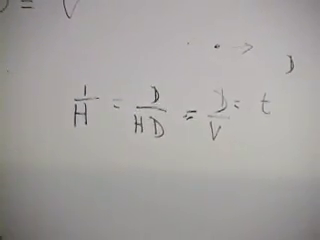
\includegraphics[width=0.66\textwidth]{lecture_08_figure_13.png}
\caption{ハッブル時間の推定値\(H^{-1}=D/(HD)=D/V\)では、後方外挿から距離が相殺される。}
\lectureframe{01:33:45}
\end{figure}

したがって、ハッブルパラメータの逆数は時間スケールであり、自動的に宇宙の正確な年齢になるわけではない。純粋に減速する物質優勢の描像では、現在の速度を逆転させ、重力が銀河を引き寄せるままにする。それらは等速の場合よりも早く出会うので、現在の\(H^{-1}\)は年齢を過大評価する。講義では約\(13.5\)億年という精密化された年齢が引用されており、ハッブル時間に近いが同一ではない。

\begin{classroomqa}
\audiencequestion{我々の銀河の内部にハッブル膨張がないなら、すべての銀河を崩壊するまで逆にたどるとはどういう意味か。}
\lecturerresponse{一様な記述は、最終的に束縛構造の実際の歴史を分解できなくなる。時間を前方に進めると、小さな揺らぎが重力的に成長して銀河や銀河団になる。文字通り逆再生した映画では、あらゆる微視的運動が逆転し、エントロピーが減少する必要がある。平均的なハッブル流れを単に逆転しても、構造形成が元に戻るわけではない。後方外挿は粗い宇宙論的推定であり、すべての恒星がその軌跡をたどる映画ではない。}
\end{classroomqa}

\begin{classroomqa}
\audiencequestion{実験は、膨張する銀河間距離と縮む物差しを区別できるか。}
\lecturerresponse{観測可能なのは無次元の比だけである。測定されるのは、銀河間の距離を原子または実験室の長さ標準で割った値が増加することである。我々は慣例的に原子・分子物理学のパラメータを固定して保持し、宇宙が膨張すると言う。銀河間の間隔を標準として選び、原子、陽子、メートル棒が縮んでいると記述することもできる。その比の物理学は変わらない。}
\end{classroomqa}

その慣例が自然なのは、棒が原子からできており、その大きさが一定に見えるパラメータによって制御されているからである。メートルは最終的に多数の微視的長さである。それらの微視的標準を固定して保持すると、\(a(t)\)が増大するというよく知られた言明が得られる。

\begin{classroomqa}
\audiencequestion{\eqref{eq:flrw-flat}は空間的一様性と平坦性に適合する唯一の計量か。}
\lecturerresponse{座標変換を除いてのみである。正確な主張は、それらの仮定と宇宙時間および共動空間座標の適切な選択の下で、計量をこの形に持ち込めるということである。別の座標系では、同じ時空がかなり異なって見えるかもしれない。}
\end{classroomqa}

\begin{classroomqa}
\audiencequestion{後方への分離がゼロに達すると、ハッブル則も速度ゼロを与える。それは銀河が出会うのを妨げるか。}
\lecturerresponse{いいえ。今日推測される\(H\)は、最後まで固定して保持されるわけではない。通常の膨張解では、\(H(t)\)はより初期の時刻にはるかに大きかった。推定値\(H_0^{-1}\)は、スケールを得るためだけに今日の速度を一様に延長して作られる。実際の\(a(t)\)、\(H(t)\)、速度は力学から求めなければならない。}
\end{classroomqa}

\section{ニュートンの球殻定理と宇宙論的力学}

力学を明らかにするには、銀河を一様な媒質に塗りつぶす。一つの銀河を原点として選び、別の銀河を共動ラベル\(x\)で指定する。この選択に物理的な特権はない。一様性は、最終的な方程式がすべての銀河の周りで同じであることを要求する。二番目の銀河の物理的半径は
\begin{equation}
  R(t)=a(t)x.
  \label{eq:radius-ax}
\end{equation}

最初は、その重力加速度を求めるには、巨大な宇宙にあるすべての銀河の引力を足し合わせる必要があるように思われる。ニュートンの球殻定理は問題を次のように崩壊させる。

\begin{proposition}[Newton's shell theorem]
逆二乗則の力と球対称な質量分布に対して、試験点を通る球の外側の物質は正味の力をゼロしか寄与しない。球の内側の物質は、囲まれた質量がすべて中心に集中しているかのように試験点に作用する。
\end{proposition}

\begin{figure}[H]
\centering
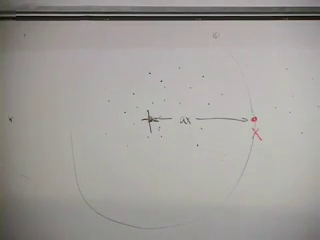
\includegraphics[width=0.70\textwidth]{lecture_08_figure_14.png}
\caption{一様な銀河分布、共動ラベル\(x\)にある試験銀河、およびその動径運動を囲まれた質量のみが制御する球。}
\lectureframe{01:50:05}
\end{figure}

\begin{figure}[H]
\centering
\begin{tikzpicture}[scale=0.94,>=Latex]
  \draw[gray!65] (0,0) circle (2.35);
  \foreach \p in {
    (-1.5,0.8),(-1.2,-0.8),(-0.8,1.5),(-0.6,0.35),(-0.3,-1.45),
    (0.15,1.05),(0.35,-0.55),(0.7,1.65),(0.9,0.45),(1.25,-0.9),
    (1.65,0.95),(-1.75,-0.2),(1.8,-0.15)} {
    \fill[black!55] \p circle (1.15pt);
  }
  \fill[blue!65!black] (0,0) circle (2pt)
    node[below left] {chosen origin};
  \fill[red!70!black] (2.35,0) circle (2.2pt)
    node[right] {test galaxy};
  \draw[->,thick] (0,0) -- (2.32,0)
    node[midway,above] {\(R=a(t)x\)};
  \draw[<->] (-2.35,-2.55) -- (2.35,-2.55)
    node[midway,below=4pt] {only the enclosed mass contributes};
\end{tikzpicture}
\caption{球殻定理の設定の明快な再構成。原点は便利な選択であり、宇宙の中心ではない。}
\end{figure}

したがって宇宙論的多体問題は、おなじみの一体問題となった。すなわち、現在の球の内部に閉じ込められた質量の引力の下で動径方向に運動する投射体である。ニュートンの方程式が、\(R=a x\) が、ひいては \(a(t)\) がどのように加速するかを決定する。講義はその計算を実行する前に意図的に止まっている。次回は、最も単純な物質優勢宇宙論を導出するのであって、その答えを幾何学的設定に密輸入するのではない。

\section{遅れて出た質問：光、ビッグバン、曲率}

正式な講義は終わったが、最後の質問はいくつかの誤解を招く描像を明らかにするものであり、付録ではなく物理学の一部である。

\begin{classroomqa}
\audiencequestion{非常に遠方の天体からの光が、宇宙がはるかに小さかったときに放出されたのなら、なぜそれは今、それほど遠くから来ているように見えるのか。また、初期宇宙がコンパクトだったのなら、なぜそのすべてが観測可能ではないのか。}
\lecturerresponse{膨張座標におけるヌル光線方程式を解かねばならない。\(a(t)\) が非常に小さいとき、\(dx/dt=1/a(t)\) は非常に大きい。光は、局所的には依然として \(c=1\) で進みながら、大きな共動区間を横切る。\(a(t)\) が大きくなるにつれて、その共動座標速度は減少する。正確な放出点と観測可能領域の大きさは、\(a(t)\) の全歴史に依存するので、数値的な答えは、特定の宇宙論が解かれるまで延期される。}
\end{classroomqa}

\begin{figure}[H]
\centering
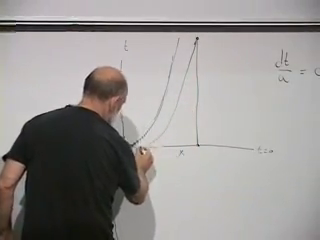
\includegraphics[width=0.72\textwidth]{lecture_08_figure_15.png}
\caption{\((x,t)\) 平面内の光線：\(a(t)\) が小さいとき共動座標ではほぼ水平であり、その後、スケール因子が大きくなるにつれて次第に急になる。}
\lectureframe{01:56:20}
\end{figure}

\eqref{eq:null-ray} を積分すると、延期された計算が明示的になる：
\begin{equation}
  \Delta x
  =\int_{t_{\mathrm e}}^{t_0}\frac{dt}{a(t)}.
  \label{eq:comoving-light-distance}
\end{equation}
\(t_{\mathrm e}\) が始まりに近づくにつれて積分が任意に大きな共動距離に達するかどうかは、\(a(t)\) の初期時間の形に依存する。\editorialnote{式 \eqref{eq:comoving-light-distance} は、黒板の式 \(dx=dt/a(t)\) の積分形である。それは、特定のスケール因子を選ぶことなく、講義が次回に割り当てる計算を明示的にする。}

\begin{figure}[H]
\centering
\begin{tikzpicture}[scale=0.92,>=Latex]
  \draw[->] (0,0) -- (6.4,0) node[right] {\(x\)};
  \draw[->] (0,0) -- (0,4.6) node[above] {\(t\)};
  \draw[thick,blue!65!black]
    plot[smooth] coordinates {(0,0.18) (1.65,0.42) (2.65,1.05)
      (3.35,2.05) (3.85,3.25) (4.05,4.25)};
  \fill[red!70!black] (4.05,4.25) circle (2pt)
    node[right] {reception today};
  \draw[dashed] (4.05,0) -- (4.05,4.25);
  \node[align=left] at (1.65,3.25)
    {\(\displaystyle \frac{dx}{dt}=\frac1{a(t)}\)\\
     large when \(a\) is small};
\end{tikzpicture}
\caption{共動座標における光線構成の整理された版。変化する傾きは座標効果であり、局所的な光速度の変化ではない。}
\end{figure}

\begin{classroomqa}
\audiencequestion{ビッグバンは物質を一点から放出したので、今では膨張する殻または環の上にあるべきなのか。}
\lecturerresponse{いいえ。このモデルは、一様で極めて高密度の空間から始まる。すべての大規模な間隔が成長する。物質は、優先的な中心から既存の空虚な空間を通って打ち出されるのではない。一様に点を付けた風船は有用な二次元の類推である。それが膨張するにつれて、すべての点の間隔が成長する一方、表面は一様に点で満たされたままである。空間はすべての正の時刻において無限でさえありうる。膨張は、それが何か他のものの内部の有限な球として始まったことを意味しない。}
\end{classroomqa}

\begin{classroomqa}
\audiencequestion{膨張の間、重力自体は弱かったのか、それとも強かったのか。}
\lecturerresponse{議論ではニュートンの定数 \(G\) を固定したままにする。それでも力は変化する。なぜなら間隔と閉じ込められた密度が変化するからである。以前は、同じ共動銀河は物理的により近く、一様な物質はより高密度だったので、重力による減速はより大きかった。これはまさに、球殻定理の計算が定量化しようとしているものである。}
\end{classroomqa}

最後に、空間曲率を膨張と混同してはならない。地球の小さな一片は、その大きさが地球の半径に比べて微小であるため平坦に見える。十分に大きな三角形を測定することにより、角度の超過を検出するか、曲率半径に下限を課すことができる。天文学は巨大な三角形を用いて同様の実験を行う。2006 年の講義で用いられた観測の言葉では、可視領域全体にわたって曲率は検出されなかったので、曲率半径はその領域より実質的に大きくなければならなかった。これは厳密に平坦な宇宙を証明するものではない。到達可能な部分がどれほど曲がりうるかに境界を与えるものである。

球について、内在的曲率は \(R^{-2}\) としてスケールする。したがって成長する球は局所的に平坦になる。同様に、一様な宇宙が非零の空間曲率をもつなら、膨張はその曲率半径を増大させ、任意の固定サイズの局所領域に見える曲率を減少させる。
\editorialnote{\(R^{-2}\) のスケーリングは、球が成長するにつれて数値的曲率が減少するという講義の記述の標準的な定量的形である。}

\begin{classroomqa}
\audiencequestion{もし空間が曲がっているなら、宇宙のある成分は収縮し、別の成分は膨張していなければならないのだろうか。}
\lecturerresponse{そうではない。正、ゼロ、負の空間曲率は、各宇宙時間スライスの幾何学を記述する。膨張または収縮は\(a(t)\)の時間発展によって支配される。曲がった宇宙は膨張しうるし、平坦な宇宙は収縮しうる。膨張は後に反転するかもしれない。ちょうど上向きに運動する投射物が落下して戻りうるように。しかし同時収縮が曲率の中に隠れているわけではない。力学上の問題は、外向きの運動が内部に含まれる質量の引力を振り切るか、落下して戻るか、それとも臨界境界上にあるかである。}
\end{classroomqa}

その脱出速度の比較が、この講義の最後の板書レベルの考えである。幾何学は計量、ハッブル則、光線方程式を与えた。ニュートンの定理は力学を一つの球の内部の質量に帰着させた。次の講義は、まさにこの講義が終わるべきところから始まる。すなわち、\(a(t)\)を決定する方程式から、そして膨張が振り切るのか、再収縮するのか、それとも刃の上に留まるのかという問いからである。

\chapter{フリードマン力学：物質、放射、真空エネルギー}

\lectureoverview{膨張宇宙の運動学は一行で述べることができる。すなわち、物理的な距離はスケール因子\(a(t)\)とともに増大する。問題は今や、その関数を決定することである。我々は平坦空間のフリードマン方程式をニュートン的なエネルギー保存から導き、まず通常の物質について解き、次に放射と真空エネルギーがなぜ全く異なる宇宙の歴史をもたらすのかを見るであろう。}

\section{説明されるべき幾何学}

固定された宇宙時刻において、大規模な宇宙は一様かつ等方に見える。銀河、銀河団、超銀河団は確かに実在する構造であるが、数億光年あるいは数十億光年のスケールでは、その分布は驚くほど一様になる。この経験的な規則性は宇宙原理と呼ばれる。その名がこれを定理にするわけではない。この原理の力は観測から来るのである。

第二の経験的事実がある。現在の精度の範囲内では、大きな空間的三角形はユークリッド三角形として振る舞う。サッカー場を測量することとの比較が有用である。ぴんと張った線がなす三角形の角の和が\(180^\circ\)になるとしても、それによって地球が大域的には平坦であることが証明されたわけではない。示されたのは、地球の曲率半径がサッカー場に比べて大きいということである。宇宙の測量も同じ論理形式をもつ。空間は非常に大きな曲率半径をもつかもしれないが、観測可能な領域では平坦であるとよく近似される。

基準となる幾何学はミンコフスキー時空であり、
\begin{equation}
  d\tau^2=dt^2-\left(dx^2+dy^2+dz^2\right).
  \label{eq:l09-minkowski}
\end{equation}
括弧は三次元におけるユークリッド距離要素にほかならない。これに対して一般相対性理論では、座標微分の係数は場である。それらは位置と時間によって変化し得るし、混合項も現れ得る。これらの計量係数は、ニュートン的重力場の相対論的な後継者である。

\begin{figure}[H]
  \centering
  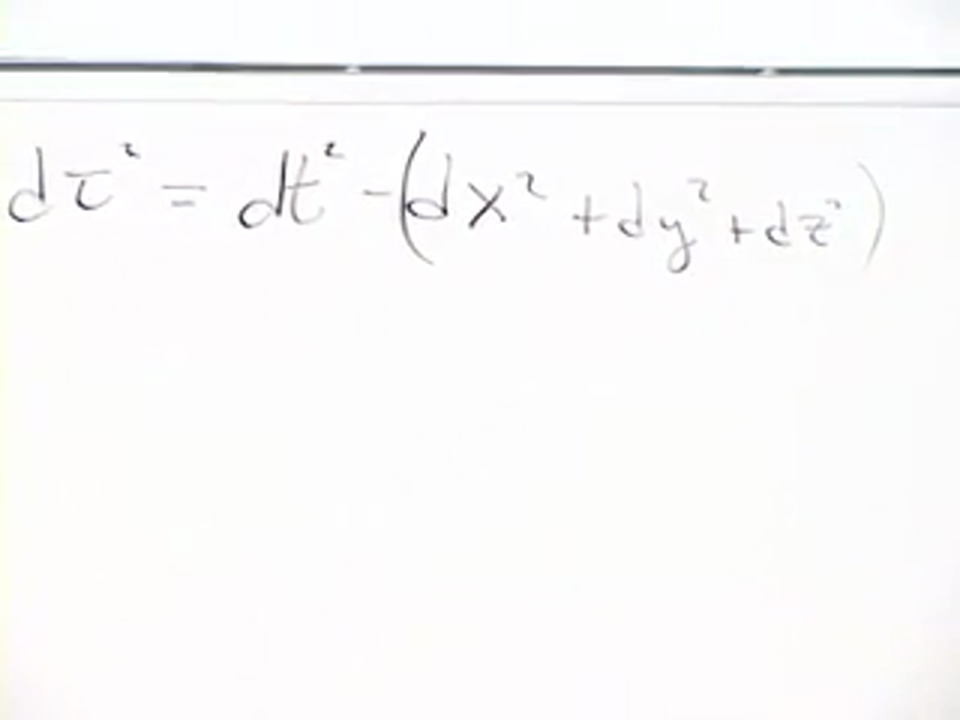
\includegraphics[width=0.72\textwidth]{lecture_09_figure_01.png}
  \caption{講義の冒頭で書かれたミンコフスキー固有時間要素。00時01分50秒のソースフレーム。}
  \label{fig:l09-minkowski-board}
\end{figure}

空間的に平坦な膨張宇宙では、一様性と等方性により、時間に依存する一つのスケール因子が残る：
\begin{equation}
  d\tau^2=dt^2-a^2(t)\left(dx^2+dy^2+dz^2\right).
  \label{eq:l09-flat-frw}
\end{equation}
我々は\(c=1\)とする単位系を用いるので、時間と長さは同じ次元をもつ。整合的な二つの規約がある。\(x,y,z\)に長さの次元を与え、\(a\)を無次元とみなすこともできるし、\(x,y,z\)を無次元のラベルとして扱い、\(a\)に長さの次元をもたせることもできる。本講義では第二の規約を用いる。それは\(a(t)\)の物理的意味を可視化するからである。

\begin{figure}[H]
  \centering
  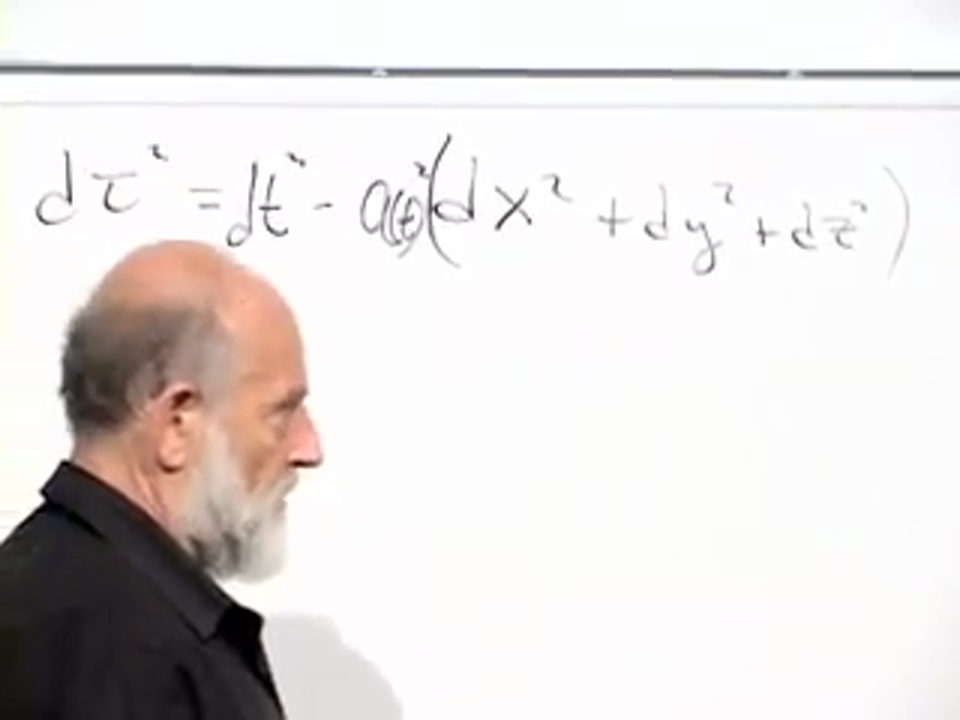
\includegraphics[width=0.72\textwidth]{lecture_09_figure_02.png}
  \caption{平坦な膨張計量であり、スケール因子がユークリッド空間的線要素に掛かる。00時09分12秒のソースフレーム。}
  \label{fig:l09-expanding-metric-board}
\end{figure}

ゴムのシートに座標が描かれていると想像しよう。座標の印はシートに貼り付いたままであるが、それらの間の物理的距離は増大する。したがって、「\(x=0\)から\(x=1\)まで」といった座標の差は、単なる一対のラベルにすぎない。その区間が表す距離は\(a(t)\)である。このスケール因子を支配する方程式を見出すことが、本講義の力学の問題である。

\section{閉じた、平坦な、開いた空間幾何学}

平坦性は観測上の単純化であり、一様性の帰結ではない。一様かつ等方な空間幾何学は三つある。正の曲率、零の曲率、負の曲率である。正の場合を理解するには、次元について正確であることが助けになる。

軌跡
\begin{equation}
  X_1^2+X_2^2=R^2
\end{equation}
は円、すなわち一次元球面\(S^1\)である。その内部を埋めたものは円板であり、二次元球体とも呼ばれる。埋め込み座標を一つ加えると
\begin{equation}
  X_1^2+X_2^2+X_3^2=R^2,
\end{equation}
通常の二次元球面\(S^2\)となる。四番目の埋め込み座標を加えると
\begin{equation}
  X_1^2+X_2^2+X_3^2+X_4^2=R^2,
  \label{eq:l09-three-sphere}
\end{equation}
三次元球面\(S^3\)となり、それ自体が三次元空間である。その四次元埋め込みを思い描くことはできないが、内在的幾何学が存在するためにその埋め込みを必要とするわけではない。

\begin{figure}[H]
  \centering
  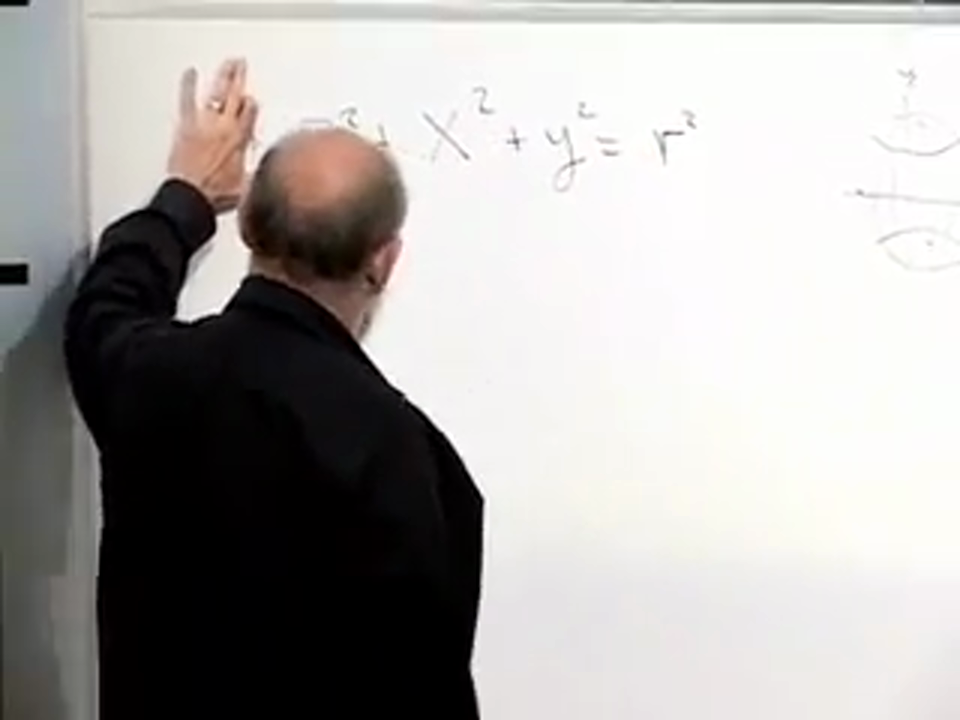
\includegraphics[width=0.72\textwidth]{lecture_09_figure_03.png}
  \caption{三次元球面を導入するために用いられた埋め込み方程式。00時16分40秒のソースフレーム。}
  \label{fig:l09-three-sphere-board}
\end{figure}

理想的な球面のどの点も他のどの点とも幾何学的に等価であり、ある点におけるどの方向も等価である。したがって球面は一様かつ等方の両方である。その半径を\(a(t)\)倍すると、空間全体が、球面上に中心を選ぶことなく膨張または収縮する。そのような宇宙を過去にたどっても、すべての物質が外部の空虚の中の一つの特別な位置に置かれるわけではない。空間全体が小さくなるので、どの点の対も近くなる。ビッグバンは空間のある一点からの爆発ではない。

正に曲がった球面上では、測地線三角形の内角の和は\(180^\circ\)より大きい。平坦な三角形の内角の和はちょうど\(180^\circ\)である。鞍面によって不完全に表される等質な負の曲率をもつ幾何学では、内角の和は\(180^\circ\)より小さい。これらの内在的テストが三つの場合を区別する。

\begin{figure}[H]
  \centering
  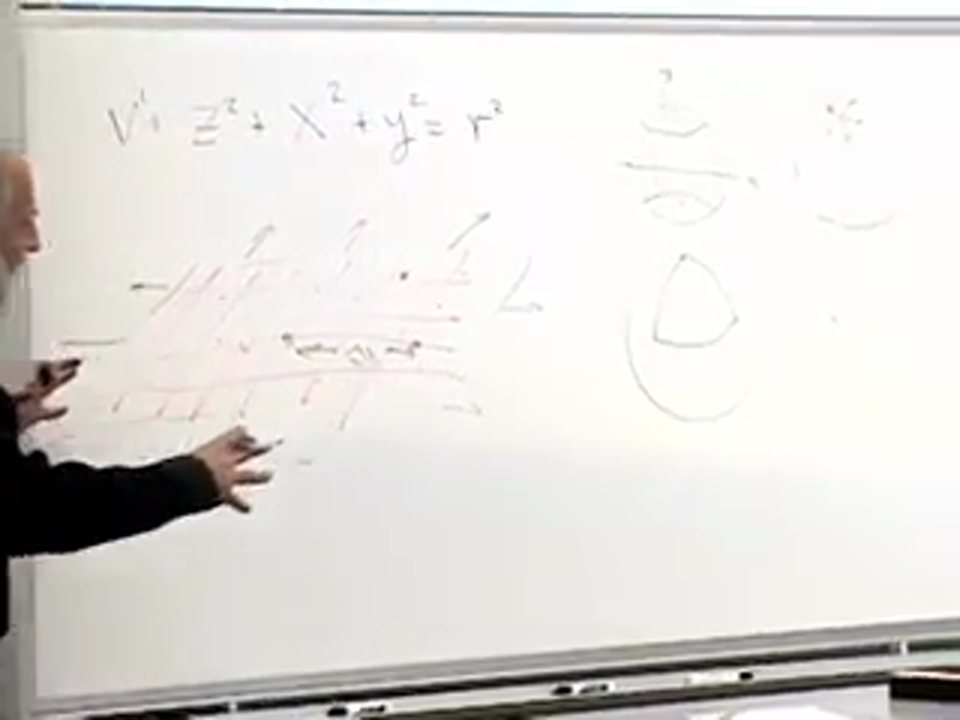
\includegraphics[width=0.72\textwidth]{lecture_09_figure_07.png}
  \caption{正、零、負の曲率をそれぞれの特徴的な三角形の形によって描いたもの。00:37:30のソースフレーム。}
  \label{fig:l09-curvature-board}
\end{figure}

完全に平坦な局所計量は、それ自体では空間が位相的に無限であることを証明しない。コンパクトな平坦位相は数学的に可能であるが、この講義では最も単純な無限ユークリッド模型を採用する。\editorialnote{この大域的位相に関する但し書きは、以降の局所的な力学のいずれにも必要ではない。}

\section{共動ラベルとハッブルの法則}

ここで膨張する平坦なシートに戻り、その上に座標格子を描こう。共動座標では、格子は大規模な物質の流れとともに膨張する。銀河、より正確には十分に粗視化された銀河団は、別の共動物体からの物理的距離が変化しても、ほぼ固定された座標ラベルを保つ。

\begin{figure}[H]
  \centering
  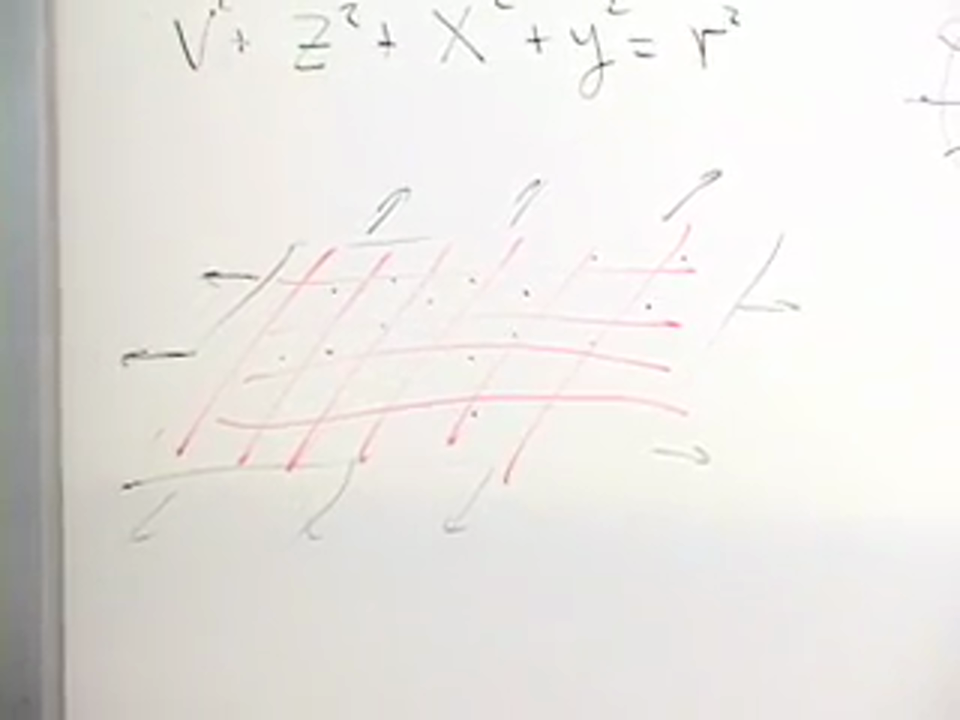
\includegraphics[width=0.72\textwidth]{lecture_09_figure_04.png}
  \caption{膨張する空間的シートに沿って運ばれる座標メッシュ。00:22:20のソースフレーム。}
  \label{fig:l09-comoving-grid-board}
\end{figure}

\(x\)軸に沿って固定された共動間隔\(\Delta x\)だけ離れた二つの物体について、それらの物理的距離は
\begin{equation}
  D(t)=a(t)\,\Delta x.
  \label{eq:l09-physical-distance}
\end{equation}
\(\Delta x\)を固定して微分すると
\begin{equation}
  v(t)=\dot a(t)\,\Delta x
      =\frac{\dot a(t)}{a(t)}D(t).
\end{equation}
次を定義すると
\begin{equation}
  H(t)\equiv\frac{\dot a(t)}{a(t)},
  \label{eq:l09-hubble-parameter}
\end{equation}
ハッブルの法則が得られる。
\begin{equation}
  v=H(t)D.
  \label{eq:l09-hubble-law}
\end{equation}
「ハッブル定数」における「定数」という語は、指定された宇宙時刻において空間全体にわたって一定であることを意味する。宇宙の歴史を通じて一定であることを意味するものではない。

\begin{figure}[H]
  \centering
  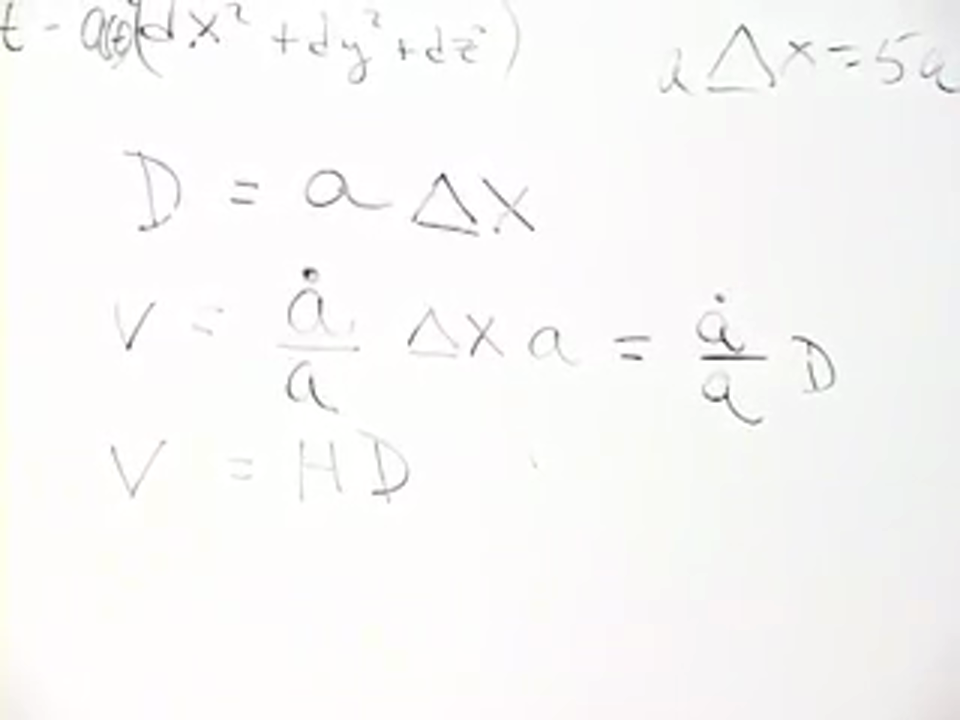
\includegraphics[width=0.72\textwidth]{lecture_09_figure_05.png}
  \caption{黒板での導出\(D=a\Delta x\)、
  \(v=(\dot a/a)D=HD\)。00:26:40のソースフレーム。}
  \label{fig:l09-hubble-board}
\end{figure}

\begin{classroomqa}
\audiencequestion{遠方の銀河がより早い時刻に見られるなら、その推定されたハッブルパラメータは本当に今日近傍で測定された値と等しいべきだろうか。}
\lecturerresponse{ルックバック時間が宇宙の年齢に比べて小さい場合に限る。適度な距離では、\(H(t)\)の変化は一つの数値が有用であるほど小さい。真に宇宙論的な距離では、我々はより早い時代を見ており、\(a\)と\(H\)の時間依存性を含めなければならない。それが、スケール因子に対する動的方程式が必要となる一つの理由である。}
\end{classroomqa}

\section{膨張する座標系におけるヌル光線}

\begin{classroomqa}
\audiencequestion{スケール因子は遠方の銀河間の光の伝播に影響するだろうか。}
\lecturerresponse{光線はヌル軌道に従うので、\(d\tau=0\)である。正の\(x\)軸に沿って進む光線では、\(dy=dz=0\)であり、膨張する計量は次を与える。
\begin{align}
  0&=dt^2-a^2(t)dx^2,
  &dt&=a(t)dx,\notag\\
  &&\frac{dx}{dt}&=\frac{1}{a(t)}.
  \label{eq:l09-null-ray}
\end{align}
座標速度は\(a(t)\)が増大するにつれて減少するが、光の局所的な物理的速度は\(c=1\)のままである。固定された座標間隔は増大する物理的距離を表す。}
\end{classroomqa}

\begin{figure}[H]
  \centering
  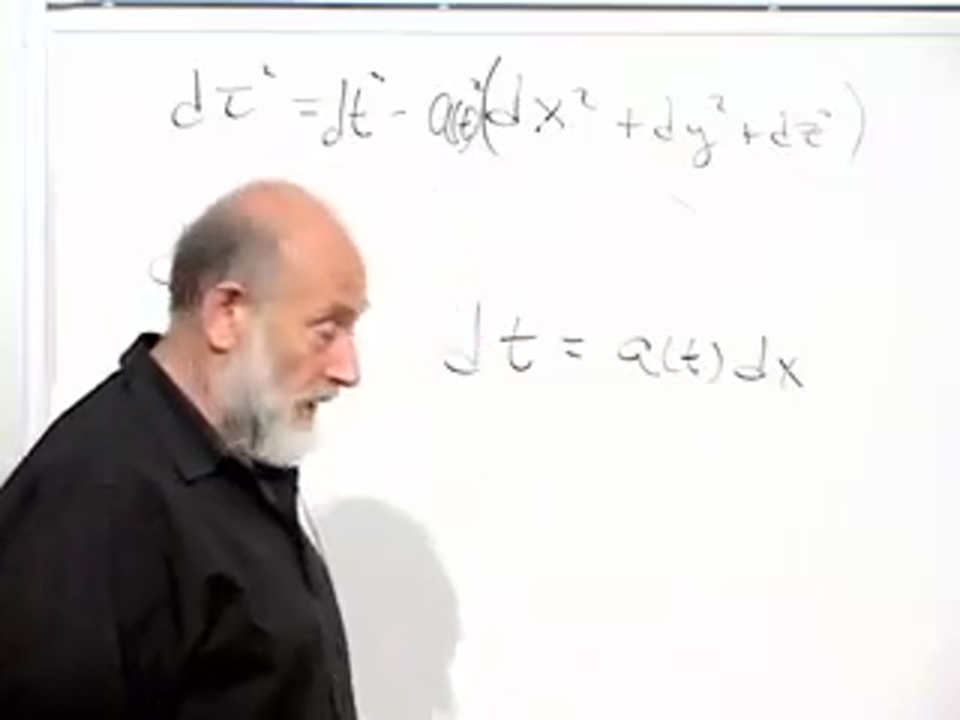
\includegraphics[width=0.72\textwidth]{lecture_09_figure_06.png}
  \caption{ヌル条件と動径方向の光伝播に対する\(dt=a(t)dx\)。00:30:54のソースフレーム。}
  \label{fig:l09-null-board}
\end{figure}

この同じ事実が「光は遠方ほど遅くなる」ように聞こえる座標を選ぶこともできるが、その場合には長さと時計がそれに対応して扱いにくい記述を帯びることになる。膨張する空間という言葉遣いの方が、自由落下するすべての観測者が同じ光速度を測定するという局所的な言明を保つので、より明快である。

\begin{classroomqa}
\audiencequestion{局所的な光の伝播と原子物理が遠方の銀河でも同じであるという証拠はあるだろうか。}
\lecturerresponse{操作的に意味があるのは無次元の比較だけである。原子の大きさを長さの単位として選び、原子的または核的な周期を時間の単位として選び、そのうえで光が選んだ長さを横切るのにそのような周期がいくつ必要かを問う。分光観測は、これらの無次元比が遠方の領域でも同じであるという言明を支持する。証拠は間接的であるが、それはまさに局所的な法則の一様性を検証する比較の一種である。}
\end{classroomqa}

観測可能な宇宙が極めて小さかったとき、光は対応する光横断単位で与えられた物理的領域を素早く横切ることができた。これは\(c\)が異なっていたことを意味しない。領域そのものが小さかったことを意味する。

\section{宇宙内部のニュートン球}

ここで運動学から力学へと移る。自分自身を原点に置き、多数の銀河と銀河団を包含するのに十分な大きさの球を描く。その境界上の銀河を一つ選ぶ。一様な宇宙では質量分布は我々のまわりで球対称であり、ニュートンの球殻定理から二つの決定的な事実が得られる：
\begin{enumerate}
  \item 選択した半径の外側にある球対称に分布した全物質は、境界の銀河に正味のニュートン力としてゼロしか及ぼさない；
  \item 球の内側にある全物質は、この動径方向の運動に対して、中心に集中しているかのように振る舞う。
\end{enumerate}
我々は静止している座標系を用いるので、以下の議論における速度と加速度は我々に対して測定される。

\begin{figure}[H]
  \centering
  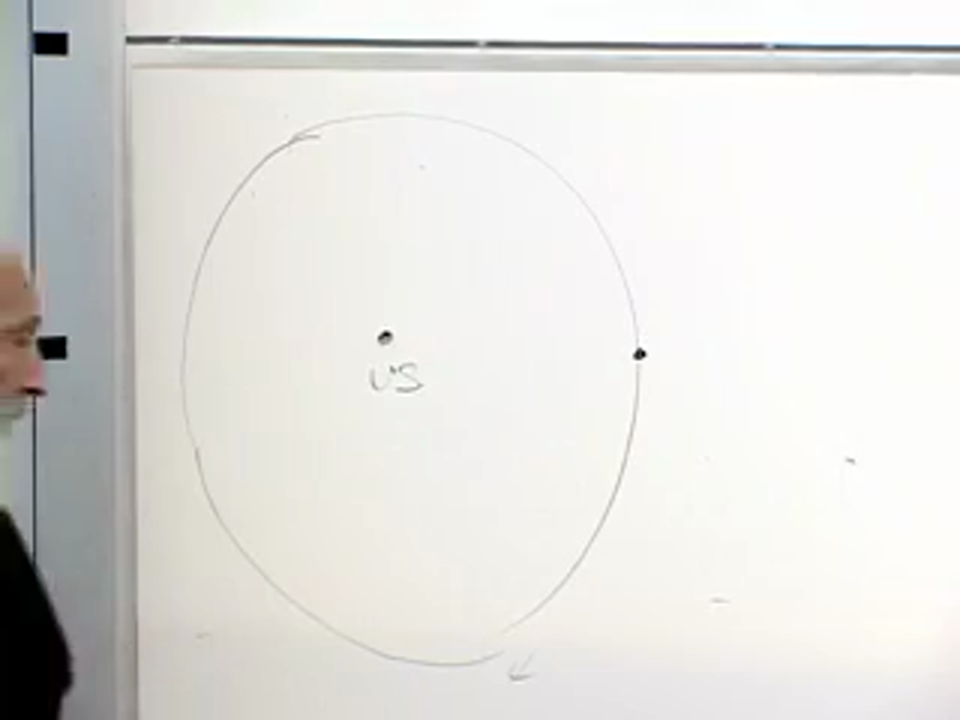
\includegraphics[width=0.72\textwidth]{lecture_09_figure_08.png}
  \caption{球殻定理の構成：我々は中心にあり、試験銀河は大きな一様球の境界上にある。00年における源フレーム：41：10。}
  \label{fig:l09-shell-board}
\end{figure}

\begin{figure}[H]
  \centering
  \begin{tikzpicture}[scale=0.92,>=Latex]
    \draw[thick] (0,0) circle (2.35);
    \fill (0,0) circle (2pt) node[below left] {us};
    \fill (2.35,0) circle (2.2pt) node[right] {test galaxy \(m\)};
    \draw[->,thick,blue!65!black] (0.18,0) -- (2.15,0)
      node[midway,above] {\(R=a(t)x\)};
    \draw[->,thick,red!65!black] (2.35,0.12) -- (3.25,0.12)
      node[midway,above] {\(v=\dot a(t)x\)};
    \node[align=center,text width=7cm] at (0,-2.85)
      {outside shells cancel;\\enclosed mass acts at the center};
  \end{tikzpicture}
  \caption{ニュートン的構成の明快な再構成。}
  \label{fig:l09-shell-clean}
\end{figure}

銀河が固定された共動座標\(x\)を持つなら、その物理的半径と速度は
\begin{equation}
  R(t)=x a(t),
  \qquad
  v(t)=x\dot a(t)=H(t)R(t).
  \label{eq:l09-radius-velocity}
\end{equation}
である。球に囲まれた質量を\(M\)、試験銀河の質量を\(m\)とする。ニュートン的エネルギーは
\begin{equation}
  E=\frac12 m v^2-\frac{GMm}{R}.
  \label{eq:l09-newtonian-energy}
\end{equation}

\begin{figure}[H]
  \centering
  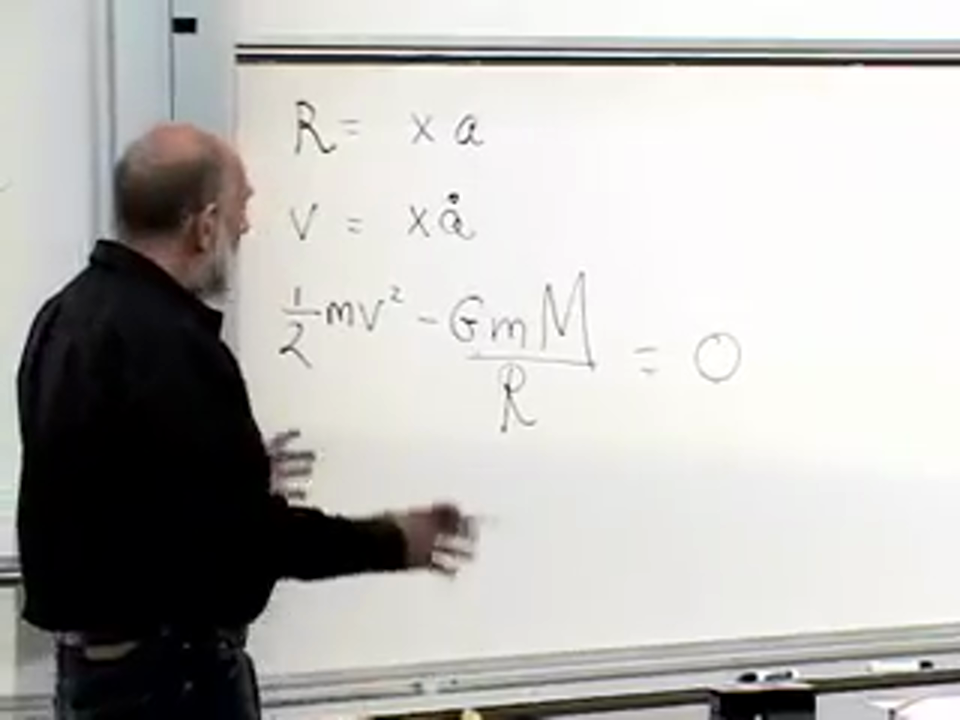
\includegraphics[width=0.72\textwidth]{lecture_09_figure_09.png}
  \caption{完全な板書の順序\(R=xa\)、\(v=x\dot a\)、および\(E=0\)に特化したニュートン的エネルギー方程式。00年における源フレーム：48：40。}
  \label{fig:l09-energy-board}
\end{figure}

エネルギーは正、ゼロ、または負であり得る。脱出と再崩壊の境界\(E=0\)から始めると、それに対して
\begin{equation}
  \frac12 v^2=\frac{GM}{R}.
  \label{eq:l09-zero-energy}
\end{equation}

\begin{classroomqa}
\audiencequestion{後退する銀河にとって全エネルギーがゼロであるとはどういう意味か？}
\lecturerresponse{それはまさに脱出速度の場合である。正のエネルギーは脱出速度を超える運動を意味し、負のエネルギーは脱出速度を下回る運動を意味し、物質のみのニュートン的描像では最終的な戻りを意味する。我々はそれらの可能性の境界から始め、平坦な方程式を導出した後に他の符号に戻る。}
\end{classroomqa}

\begin{classroomqa}
\audiencequestion{囲まれた質量\(M\)は球が膨張するにつれて変化するか？}
\lecturerresponse{いいえ。球は共動しているので、同じ粒子がその内部にとどまる。その物理的体積は増大し密度は低下するが、その全囲まれた質量は固定されたままである。\(M\)と\(\rho(t)\)のこの区別は本質的である。}
\end{classroomqa}

一様密度\(\rho(t)\)に対して、
\begin{equation}
  M=\frac{4\pi}{3}\rho(t)R^3.
  \label{eq:l09-enclosed-mass}
\end{equation}
\eqref{eq:l09-zero-energy}への代入により
\begin{equation}
  \frac12 v^2
  =\frac{G}{R}\left(\frac{4\pi}{3}\rho R^3\right).
  \label{eq:l09-enclosed-energy}
\end{equation}

\begin{figure}[H]
  \centering
  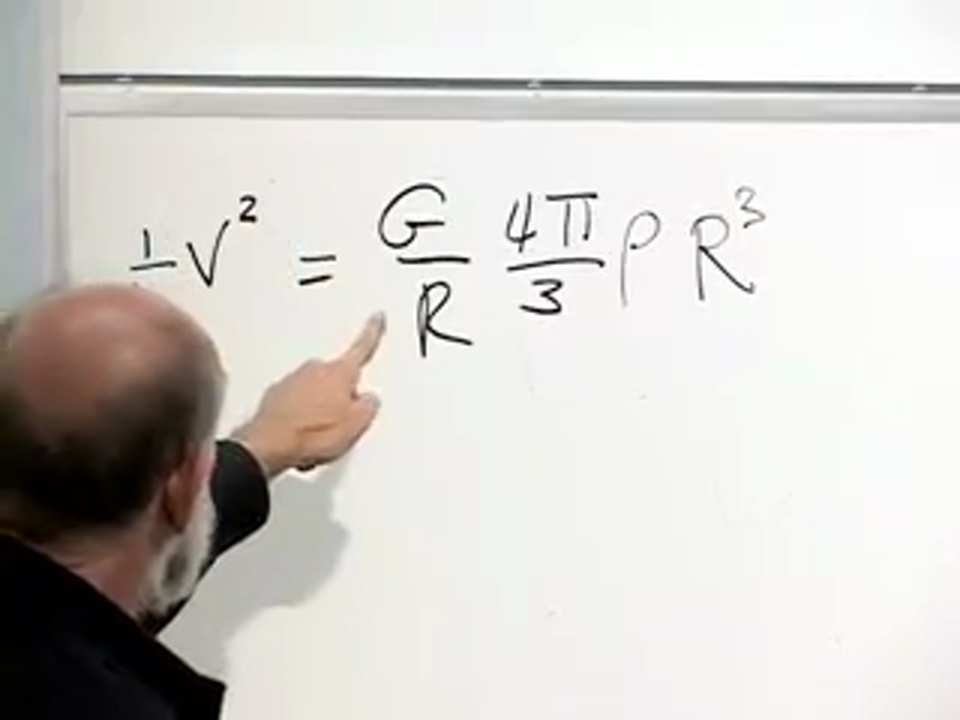
\includegraphics[width=0.72\textwidth]{lecture_09_figure_10.png}
  \caption{ゼロエネルギー方程式における囲まれた質量の代入。
  00年における源フレーム：54：16.060。}
  \label{fig:l09-enclosed-mass-board}
\end{figure}

\(v=HR\)を用いると、
\begin{align}
  \frac12 H^2R^2
    &=\frac{4\pi G}{3}\rho R^2,\\
  H^2
    &=\frac{8\pi G}{3}\rho.
\end{align}
が得られる。したがって、ゼロエネルギーで空間的に平坦な膨張則は
\begin{equation}
  \boxed{\left(\frac{\dot a}{a}\right)^2
  =\frac{8\pi G}{3}\rho(t)}.
  \label{eq:l09-flat-friedmann}
\end{equation}
である。\(R^2\)の相殺は偶然ではない。一様な宇宙は、どの共動銀河を試験対象として選んでも同じ\(H(t)\)を与えなければならない。

\begin{figure}[H]
  \centering
  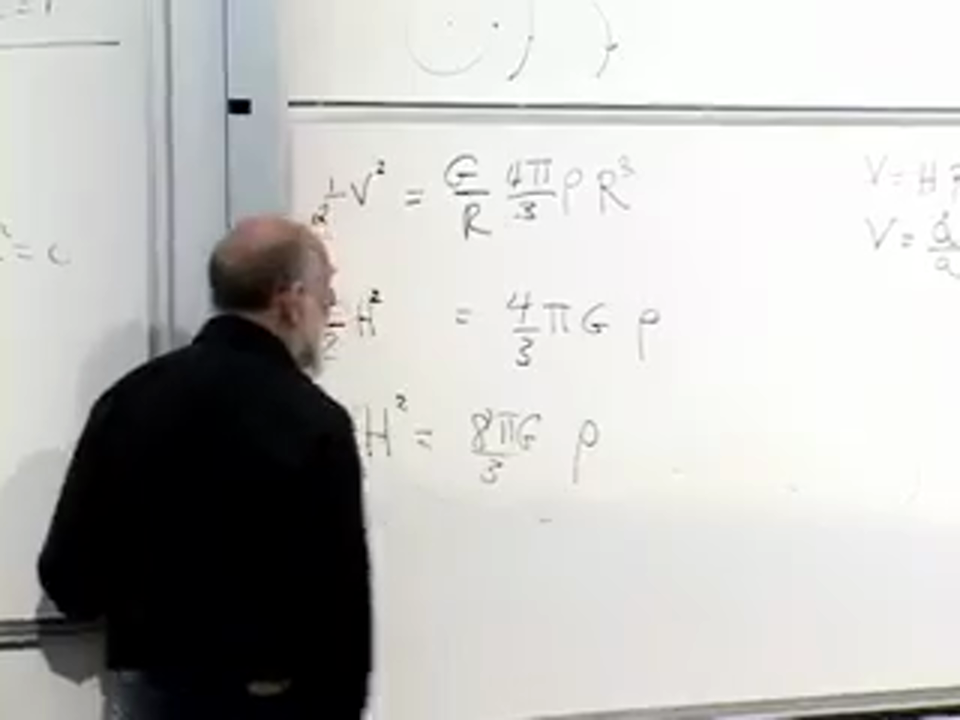
\includegraphics[width=0.72\textwidth]{lecture_09_figure_11.png}
  \caption{半径の相殺と、その結果として得られる平坦なフリードマン関係が板書に示されている。00年における源フレーム：57：30。}
  \label{fig:l09-friedmann-board}
\end{figure}

\begin{classroomqa}
\audiencequestion{ゼロエネルギー関係の証拠はあるか？}
\lecturerresponse{両辺は観測的に推論できる：\(H\)は後退データから、\(\rho\)は恒星、ガス、暗黒物質、真空エネルギーを考慮することによって。講義当時の比較では、両辺は約パーセントの精度で一致していた。この限定は重要である：すべての形態のエネルギーを含めなければならず、後の真空エネルギーの議論は素朴な脱出速度の解釈を変える。}
\end{classroomqa}

単位\(c=1\)では、質量密度とエネルギー密度は同じ単位を持つ。したがって記号\(\rho\)は、議論中の成分に適した全エネルギー密度を表す。

\section{通常の物質と3分の2の法則}

方程式\eqref{eq:l09-flat-friedmann}は、\(\rho(t)\)がどのように変化するかを知るまで閉じない。まず、共動する直方体の箱をゆっくり運動する非相対論的粒子で満たす。その座標次元は固定されているが、その物理的体積は
\begin{equation}
  V(t)=a^3(t)\,\Delta x\,\Delta y\,\Delta z.
\end{equation}
として増大する。箱の中の粒子数と静止質量は固定されたままなので、
\begin{equation}
  \rho_{\mathrm m}(t)=\frac{C_{\mathrm m}}{a^3(t)}.
  \label{eq:l09-matter-dilution}
\end{equation}
現在の時代\(t_0\)に規格化すると、
\begin{equation}
  \frac{\rho_{\mathrm m}(t)}{\rho_{\mathrm m,0}}
  =\left(\frac{a_0}{a(t)}\right)^3.
  \label{eq:l09-matter-normalized}
\end{equation}

\begin{figure}[H]
  \centering
  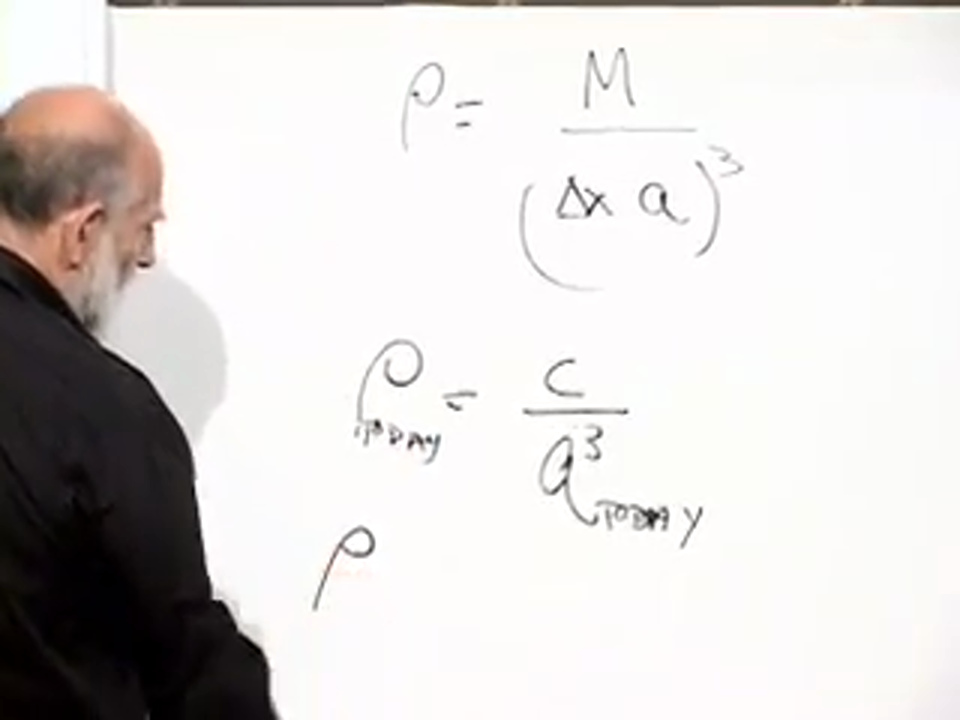
\includegraphics[width=0.72\textwidth]{lecture_09_figure_12.png}
  \caption{物質密度、その\(a^{-3}\)希釈、および現在の規格化。01年における源フレーム：04：47.940。}
  \label{fig:l09-density-board}
\end{figure}

\begin{classroomqa}
\audiencequestion{現在の宇宙の粗いエネルギー密度はどれほどで、通常の原子だけでそれを賄えるのか。}
\lecturerresponse{可視バリオン物質の数え上げでは、答えの一部しか得られない。暗黒物質と暗黒エネルギーも等価な質量エネルギーとして表さなければならない。講義では、立方メートルあたり原子一個から水素質量数十個分に及ぶ粗い尺度が引用され、精密な目録よりも桁の程度が強調されている。}
\end{classroomqa}

\eqref{eq:l09-matter-dilution}を\eqref{eq:l09-flat-friedmann}に代入し、すべての時間に依存しない因子を正の定数\(C\)に吸収すると、
\begin{equation}
  \left(\frac{\dot a}{a}\right)^2=\frac{C}{a^3},
  \qquad
  \dot a^2=\frac{C}{a}.
  \label{eq:l09-matter-ode}
\end{equation}
これを解く透明な方法が二つある。冪則の試行解\(a=K t^p\)は
\begin{equation}
  p-1=-\frac{p}{2},
  \qquad p=\frac23.
\end{equation}
を要求する。同値に、展開する平方根の分枝を取って積分すると、
\begin{equation}
  a^{1/2}\frac{da}{dt}=\sqrt C,
  \qquad
  \int a^{1/2}da=\sqrt C\int dt,
\end{equation}
となるので、時間のビッグバン起源を選んだ後、
\begin{equation}
  a^{3/2}\propto t,
  \qquad
  \boxed{a(t)\propto t^{2/3}}.
  \label{eq:l09-matter-solution}
\end{equation}
となる。ライブの導出では係数を合わせる際に一時的に因子を失うが、その後積分に戻って指数を検証する。ノートは検算を保持するが、表示するのは訂正された代数のみである。

\begin{figure}[H]
  \centering
  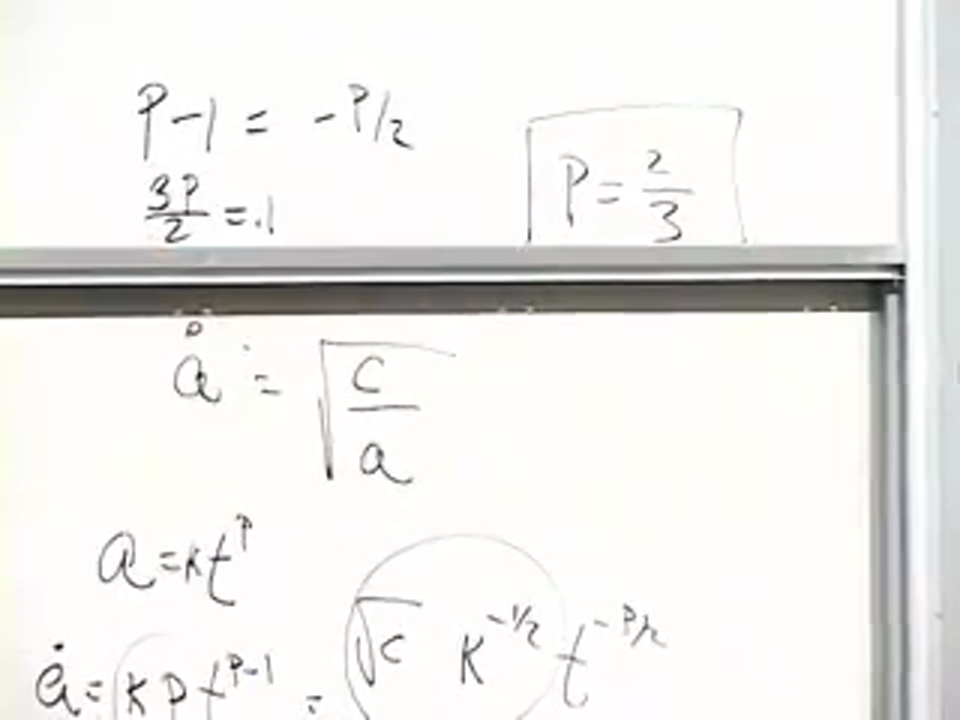
\includegraphics[width=0.72\textwidth]{lecture_09_figure_13.png}
  \caption{冪則の試行解と枠で囲まれた指数\(p=2/3\)。01のソースフレーム：13：05。}
  \label{fig:l09-matter-solution-board}
\end{figure}

解を微分すると
\begin{equation}
  H(t)=\frac{\dot a}{a}=\frac{2}{3t}.
  \label{eq:l09-matter-hubble}
\end{equation}
が得られる。ハッブルパラメータは過去においてより大きかった。したがって、無視できないルックバック時間が見えるほど遠くを見るとき、今日の\(H_0\)を変えずに局所的な線形関係を延長してはならない。

\begin{figure}[H]
  \centering
  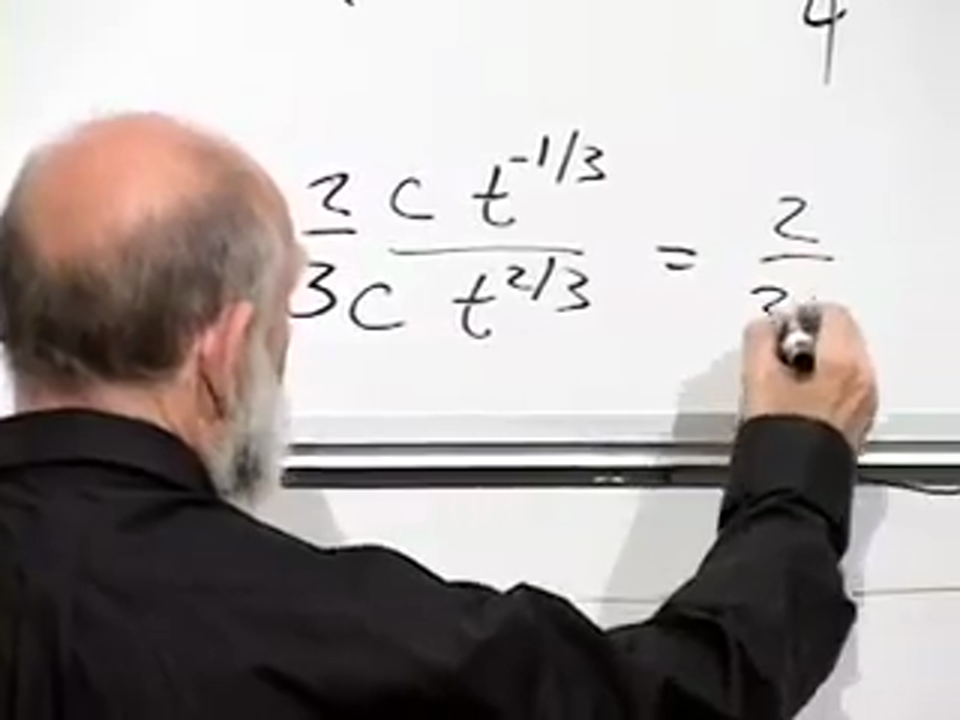
\includegraphics[width=0.72\textwidth]{lecture_09_figure_14.png}
  \caption{\(a\propto t^{2/3}\)に対して\(\dot a/a\)を取ると\(H=2/(3t)\)が得られる。01のソースフレーム：20：42。}
  \label{fig:l09-hubble-time-board}
\end{figure}

\section{エネルギーの符号と空間曲率}

ニュートン的な推論は平坦なゼロエネルギーの場合を貫いて我々を導いてきた。一般相対性理論は、球殻定理だけからは得られない事実を付け加える。ニュートン流の比エネルギーの符号は空間曲率の符号に対応する。
\begin{center}
\begin{tabular}{@{}>{\raggedright\arraybackslash}p{0.20\linewidth}
                    >{\raggedright\arraybackslash}p{0.29\linewidth}
                    >{\raggedright\arraybackslash}p{0.37\linewidth}@{}}
  \toprule
  全エネルギー & 空間曲率 & 物質のみの運命 \\
  \midrule
  正 & 負（開） & 永遠に膨張する \\
  ゼロ & ゼロ（平坦） & 脱出境界に近づく \\
  負 & 正（閉） & 膨張し、転回し、再収縮する \\
  \bottomrule
\end{tabular}
\end{center}
最後の列は真空エネルギーがないことを仮定している。発射体の類推では、正のエネルギーは脱出速度より上、ゼロはちょうど脱出速度、負は脱出速度より下を意味する。アインシュタイン方程式はこれら三つの場合をそれぞれ開いた、平坦な、閉じた空間幾何学と同一視する。

\section{光子と1/2則}

物質の法則\(\rho\propto a^{-3}\)は、各粒子のエネルギーがほぼ固定されている一方で数密度が減少すると仮定している。光子はその仮定に反する。光子に対しては、
\begin{equation}
  E=h\nu=\frac{hc}{\lambda}.
\end{equation}
膨張はその波長をスケール因子に比例して伸ばし、
\begin{equation}
  \lambda\propto a,
  \qquad E\propto a^{-1}.
\end{equation}
光子数密度は依然として\(a^{-3}\)のように減少し、各光子のエネルギーがさらに\(a^{-1}\)の因子を一つ寄与する。したがって
\begin{equation}
  \boxed{\rho_{\mathrm r}(t)\propto a^{-4}(t)}.
  \label{eq:l09-radiation-dilution}
\end{equation}

ギター弦の類推は物理的描像を捉えている。弦を弾き、次にその振動部分を長くすると、波長は長くなり音は下がる。膨張する共動箱の中の光子モードも同様に振る舞う。この描像を逆向きにたどると、圧縮は波長を短くし光子エネルギーを高める。

\begin{figure}[H]
  \centering
  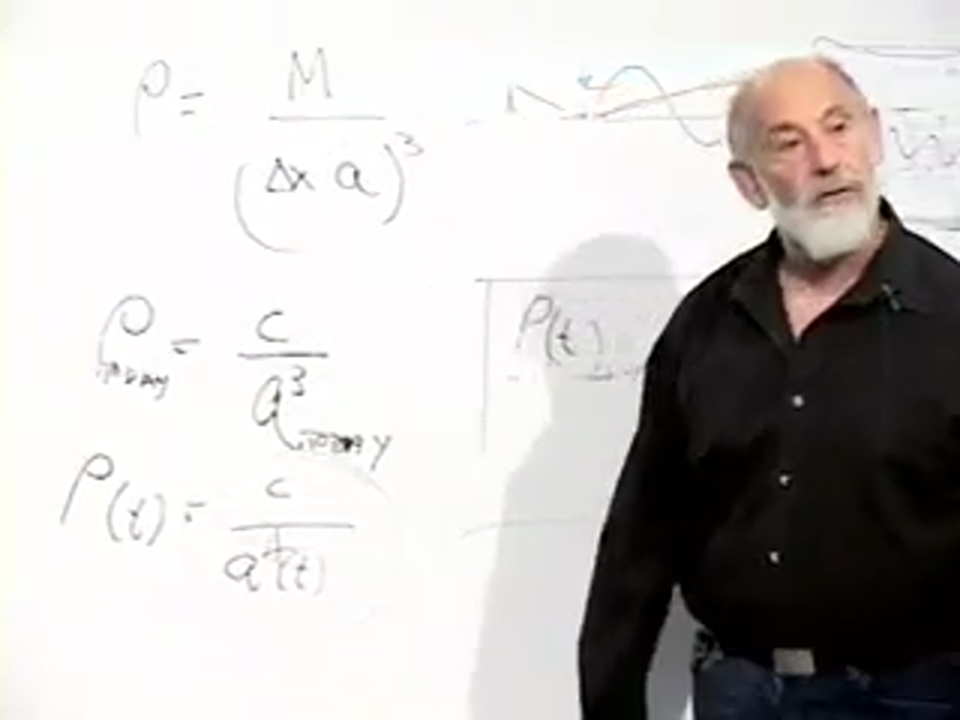
\includegraphics[width=0.72\textwidth]{lecture_09_figure_15.png}
  \caption{物質密度の関係を黒板で放射のスケーリング\(\rho_{\mathrm r}\propto a^{-4}\)へ拡張したもの。01のソースフレーム：29：20。}
  \label{fig:l09-radiation-board}
\end{figure}

平坦なフリードマン方程式で\(\rho_{\mathrm r}\propto a^{-4}\)を用いると
\begin{equation}
  \left(\frac{\dot a}{a}\right)^2=\frac{C_{\mathrm r}}{a^4},
  \qquad
  \dot a\propto a^{-1},
\end{equation}
が得られ、したがって
\begin{equation}
  \boxed{a(t)\propto t^{1/2}}.
  \label{eq:l09-radiation-solution}
\end{equation}
となる。これは\(t^{2/3}\)よりゆっくり成長する。十分に過去へさかのぼると、\(a\)が減少するにつれて\(a^{-4}\)が\(a^{-3}\)より速く上昇するため、放射が通常の物質を支配しなければならない。講義では物質と放射の交差を、スケール因子が今日よりおよそ千倍小さかった時代のあたりに置いている。その交差より前、宇宙は放射支配であり、その後、長い期間にわたって物質支配であった。

\section{真空エネルギーと指数関数的膨張}

真空エネルギーは逆のスケーリング挙動を示す。その密度は空の空間の性質であり、宇宙が膨張しても薄まらない：
\begin{equation}
  \rho_\Lambda=\text{constant}.
  \label{eq:l09-vacuum-density}
\end{equation}
通常の物質と放射は過去に向かってより密になるが、この項はそうならない。したがって初期宇宙ではより重要でなく、他の成分が薄まるにつれてより重要になる。講義では、真空エネルギーが今日の宇宙エネルギー密度のおよそ\(70\%\)を供給するという当時の推定を用いている。

\(\rho_\Lambda\) を一定とすると、式 \eqref{eq:l09-flat-friedmann} は一定の膨張率を与える。
\begin{equation}
  H_\Lambda=\sqrt{\frac{8\pi G}{3}\rho_\Lambda},
  \qquad
  \frac{\dot a}{a}=H_\Lambda.
\end{equation}
したがって
\begin{equation}
  \boxed{a(t)=a(t_i)e^{H_\Lambda(t-t_i)}}.
  \label{eq:l09-vacuum-solution}
\end{equation}

\begin{figure}[H]
  \centering
  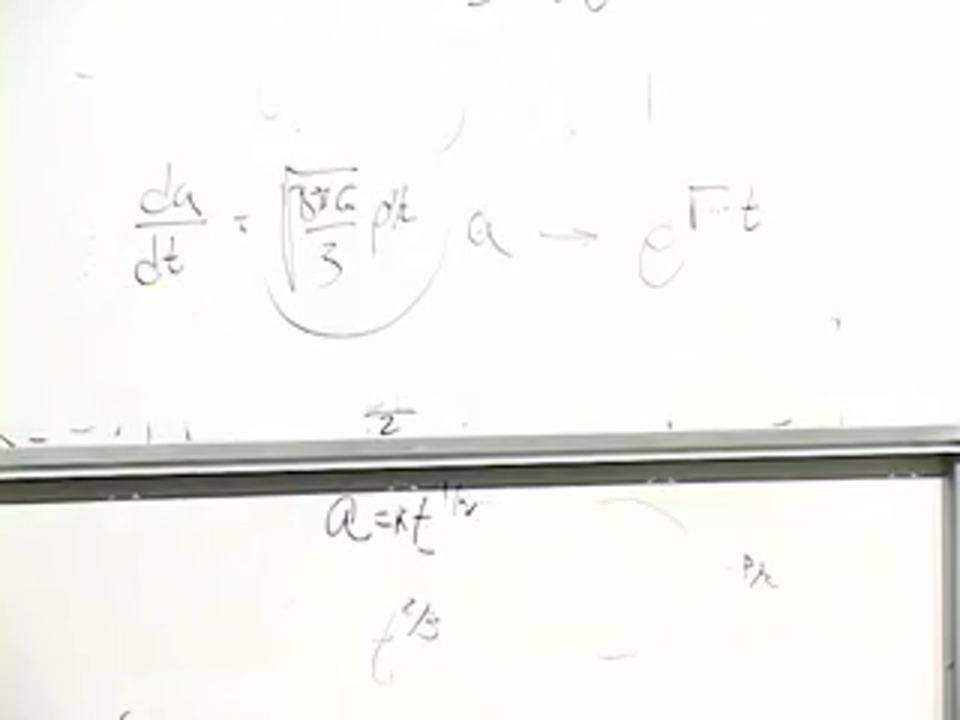
\includegraphics[width=0.72\textwidth]{lecture_09_figure_16.png}
  \caption{指数関数的膨張を導く定数密度の式。
  ソースフレーム 01:35:48。}
  \label{fig:l09-vacuum-board}
\end{figure}

講義で引用された観測スケールでは、宇宙の線形サイズはおよそ百億年から百二十億年で二倍になる。この小さく非零の真空密度の起源は依然として説明されていない。その存在と膨張への影響は経験的事実である。

\begin{classroomqa}
\audiencequestion{この議論において、真空エネルギーはダークエネルギーと同じものか。}
\lecturerresponse{はい。ここで「ダークエネルギー」とは一定の真空エネルギー密度、等価的には宇宙定数を指す。より一般的な時間依存ダークエネルギーモデルも想像できるが、それらはこの講義の計算の一部ではない。}
\end{classroomqa}

\section{膨張する宇宙が光を赤方偏移させる仕組み}

\begin{classroomqa}
\audiencequestion{光子は、我々が膨張する共動座標を選んだこと、したがって光子がエネルギーを下げることを、どうして知り得るのか。}
\lecturerresponse{光子は我々のラベルに反応しない。光子は、物理的間隔が変化する幾何学の中を伝播する。物理的サイズが二倍になる領域を占める波連は、二倍の波長を獲得する。共動座標はこの伸張を簡潔に記述するにすぎず、それを引き起こすのではない。}
\end{classroomqa}

\begin{classroomqa}
\audiencequestion{今日我々に到達する背景光子はどこから来るのか。}
\lecturerresponse{より遠くを見ることはより昔を見ることである。やがて我々は、宇宙の物質が電離プラズマであった時代を見る。それは自由な荷電粒子によって光子が繰り返し散乱されるため不透明である。光子が最後に自由に我々へと旅することができた境界は、観測者を取り囲む球として現れる。すなわち最終散乱面である。}
\end{classroomqa}

\begin{figure}[H]
  \centering
  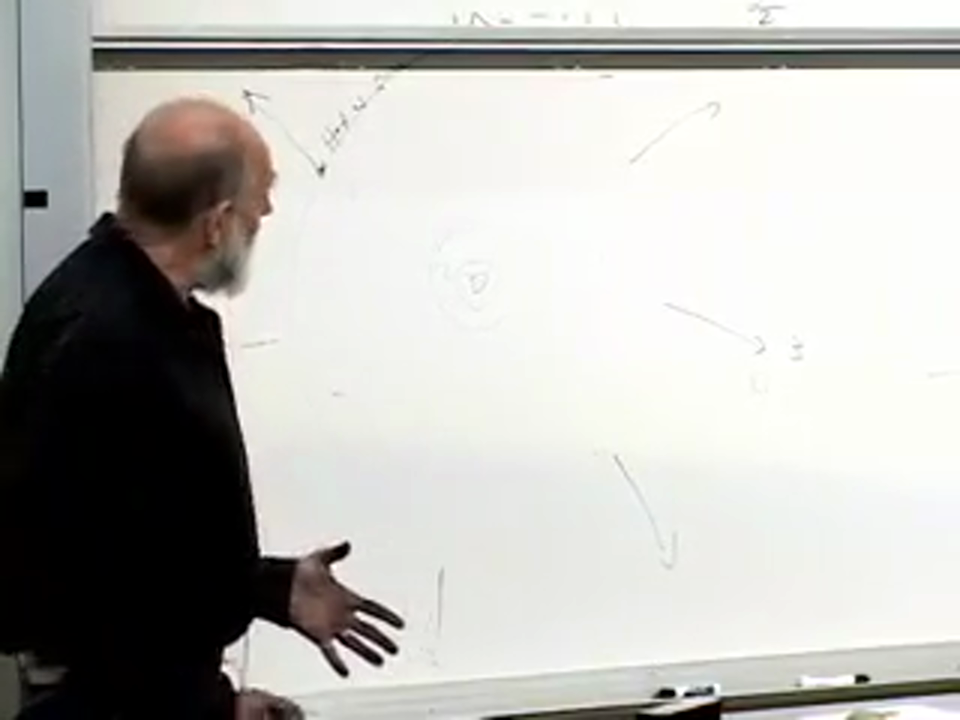
\includegraphics[width=0.72\textwidth]{lecture_09_figure_17.png}
  \caption{最終散乱面と次第に遠くなる殻の観測者中心のスケッチ。ソースフレーム 01:42:05。}
  \label{fig:l09-last-scattering-board}
\end{figure}

\begin{figure}[H]
  \centering
  \begin{tikzpicture}[scale=0.9,>=Latex]
    \fill (0,0) circle (2pt) node[below] {observer};
    \draw[thick,orange!70!black] (0,0) circle (2.55);
    \node[orange!70!black,align=center] at (0,3.05)
      {surface of last scattering};
    \foreach \a in {25,75,145,210,285,335}{
      \draw[->,blue!60!black] ({2.55*cos(\a)},{2.55*sin(\a)}) --
        ({1.7*cos(\a)},{1.7*sin(\a)});
    }
    \draw[decorate,decoration={snake,amplitude=1.5pt,segment length=7pt},
      red!65!black,thick,->] (-2.5,0) -- (-0.15,0);
    \node[red!65!black,below] at (-1.35,-0.15)
      {redshifted photon};
  \end{tikzpicture}
  \caption{最終散乱の描像の明瞭な再構成。}
  \label{fig:l09-last-scattering-clean}
\end{figure}

その放射は高温プラズマに特徴的なスペクトルで放出され、およそ千倍長い波長で我々に到達する。講義のドップラー的表現では、遠方の放射面は速やかに後退し、その放射は強く赤方偏移する。幾何学的表現では、波は伝播の間に伸張する。両方の描像は同じ関係を表しており、\begin{equation}
  1+z=\frac{\lambda_0}{\lambda_{\mathrm{em}}}
      =\frac{a_0}{a_{\mathrm{em}}}.
  \label{eq:l09-cosmological-redshift}
\end{equation}
\editorialnote{式\eqref{eq:l09-cosmological-redshift}は、講義の伸張およびドップラーによる記述の標準的な定量的形式である。}

より早い観測時代には、最終散乱球は対応する描像においてより近くにあり、観測される背景光子はより赤方偏移が小さく、したがってより高エネルギーであったであろう。宇宙時間が進むにつれて、その初期プラズマから共動観測者に到達する光子は次第に長い波長を持つ。

\section{赤方偏移した光子のエネルギーはどこへ行くのか。}

\begin{classroomqa}
\audiencequestion{光子はエネルギー \(h\nu_{\mathrm{em}}\) で放出され、より少ないエネルギーで赤方偏移して到達する。その差はどうなったのか。}
\lecturerresponse{ニュートン的導出はエネルギー方程式として始まった。その宇宙論的形式は膨張率を物質エネルギー密度に関係づけるので、物質エネルギーと膨張を別々に保存される会計として扱うことはできない。講義は、失われた光子エネルギーが膨張の運動学的な帳簿に入ると記述する。放射で満たされたピストンがこの類推を具体的にする。放射圧がピストンを外側へ押し、光子の波長が増大し、失われたエネルギーが力学的仕事とピストンの運動エネルギーになる。}
\end{classroomqa}

\begin{figure}[H]
  \centering
  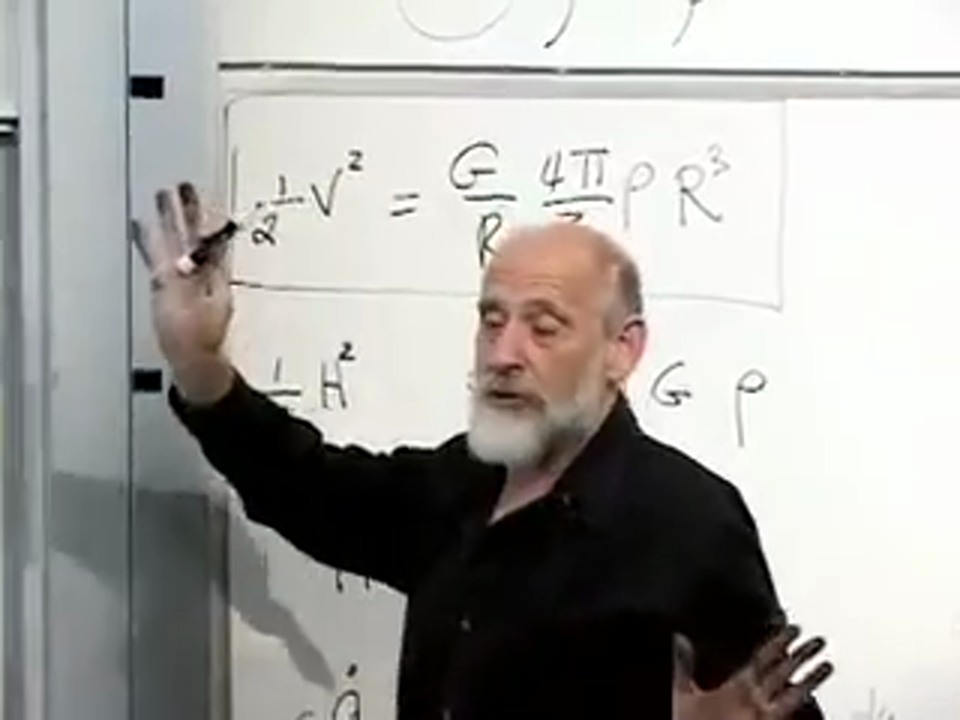
\includegraphics[width=0.72\textwidth]{lecture_09_figure_18.png}
  \caption{黒板は、枠で囲まれたニュートン的エネルギー方程式を対応するフリードマン方程式の上に置いている。ソースフレーム 01:44:42。}
  \label{fig:l09-energy-bookkeeping-board}
\end{figure}

\begin{classroomqa}
\audiencequestion{何が放射エネルギーを膨張に結合するのか。}
\lecturerresponse{圧力である。可動ピストンを備えたシリンダーでは、光子が壁に運動量を移す。ピストンが動くにつれて、放射は仕事をし、その波長は増大し、そのエネルギーは減少する。一様に膨張する宇宙には文字通りの外側のピストンはないが、\(p\,dV\) の類推は、放射のエネルギー密度が単なる数密度の希釈よりも速く減少する理由を説明する。}
\end{classroomqa}

\begin{figure}[H]
  \centering
  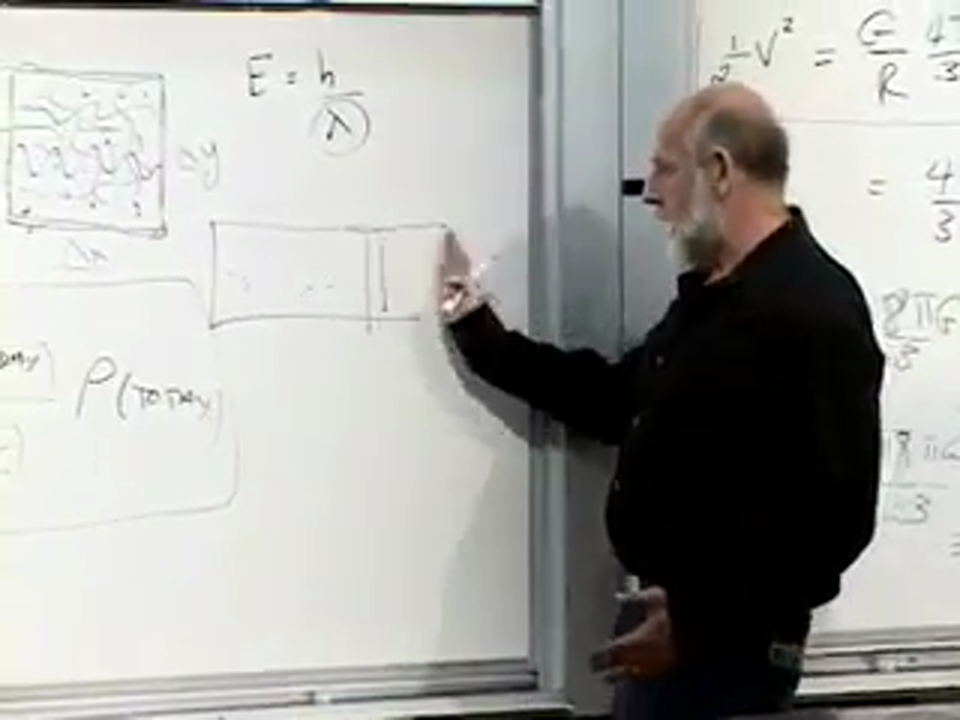
\includegraphics[width=0.72\textwidth]{lecture_09_figure_19.png}
  \caption{圧力仕事を可視化するために用いられる、可動の光子で満たされたピストン。ソースフレーム 01:46:40。}
  \label{fig:l09-piston-board}
\end{figure}

\begin{figure}[H]
  \centering
  \begin{tikzpicture}[scale=0.92,>=Latex]
    \draw[thick] (0,0) rectangle (5.3,2.6);
    \draw[very thick] (4.25,0) -- (4.25,2.6);
    \draw[very thick] (4.25,1.3) -- (5.25,1.3);
    \draw[->,thick,red!65!black] (5.25,1.3) -- (6.2,1.3)
      node[right] {moving piston};
    \foreach \y in {0.55,1.3,2.05}{
      \draw[decorate,decoration={snake,amplitude=1.4pt,segment length=6pt},
        blue!65!black,->] (0.35,\y) -- (3.9,\y);
    }
    \node at (2.15,-0.45) {radiation does \(p\,dV\) work};
  \end{tikzpicture}
  \caption{放射ピストンの類推の整理された再構成。}
  \label{fig:l09-piston-clean}
\end{figure}

一般相対性理論におけるエネルギーには注意が必要である。一般的な膨張時空では、孤立したニュートン系のエネルギーに相当する、一意に保存される大域的なエネルギーが存在する必要はない。局所的な応力エネルギーの保存は依然として成り立ち、一様な流体に対しては連続の式
\begin{equation}
  \dot\rho+3H(\rho+p)=0,
  \label{eq:l09-continuity}
\end{equation}
が得られる。この式には、物質と放射のスケーリング則の背後にある圧力仕事の項が含まれている。\editorialnote{式\eqref{eq:l09-continuity}は、講義で意図的にニュートン的なエネルギー収支の類推の基礎となっている、正確な局所的一般相対論的表現である。}

真空エネルギーはこの難問を特に鋭くする。その密度は体積が増大しても一定に保たれるため、共動領域内の全真空エネルギーは増加する。その負の圧力は重力源の一部であり、加速膨張を駆動する。したがって、幾何学と圧力仕事を含めずに、素朴な「共動箱の中の物質エネルギー」の独立した保存を要求すべきではない。

\section{なぜスケール因子を時間項から除くことができるのか}

\begin{classroomqa}
\audiencequestion{なぜスケール因子は計量の空間部分には掛かるが、時間部分には掛からないのか。}
\lecturerresponse{それは時間座標の選び方である。共形時間座標\(t\)から出発し、
\begin{equation}
  d\tau^2=A^2(t)\left(dt^2-dx^2\right).
\end{equation}
とする。新しい宇宙時間\(T\)を
\begin{equation}
  dT=A(t)\,dt.
\end{equation}
によって定義する。すると
\begin{equation}
  d\tau^2=dT^2-A^2\bigl(t(T)\bigr)dx^2.
\end{equation}
となる。時間微分の前の共通因子は消え、物理的なスケール因子は空間項に残る。}
\end{classroomqa}

\begin{figure}[H]
  \centering
  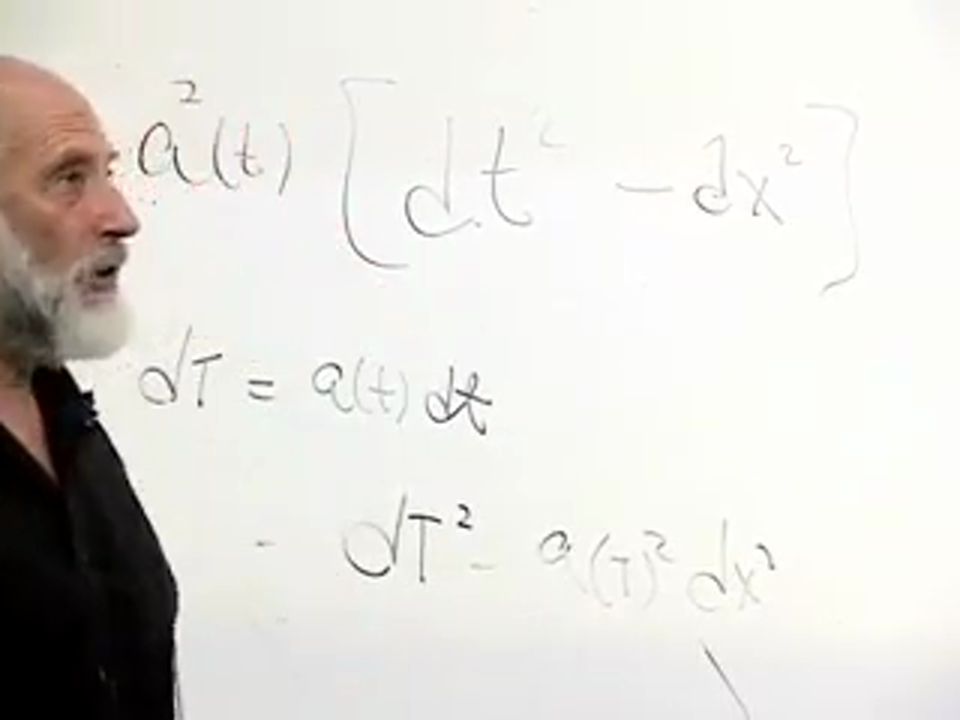
\includegraphics[width=0.72\textwidth]{lecture_09_figure_20.png}
  \caption{共形時間を宇宙時間に変換する時間の再定義\(dT=A(t)dt\)。01におけるソースフレーム：51：05。}
  \label{fig:l09-time-reparam-board}
\end{figure}

\section{曲率、真空エネルギー、宇宙の運命}

\begin{classroomqa}
\audiencequestion{もし宇宙が正の曲率を持っていたなら、銀河が我々に向かって来るのをすでに見るべきではないか。}
\lecturerresponse{必ずしもそうではない。脱出速度を下回る速度で打ち上げられた物体は、まず外側へ進み、転回点に達し、その後になって初めて落下して戻る。我々は宇宙を膨張段階で観測している。真空エネルギーがなければ、正の曲率を持つ物質宇宙は最終的に再収縮するであろう。十分に大きな正の真空エネルギーはその転回を妨げ、観測値は、小さな空間曲率にかかわらず長期的な膨張を指数的にするのに十分な大きさであるように見える。}
\end{classroomqa}

指数的な未来はエネルギーの楽園ではない。恒星は最終的に燃え尽き、物質と放射の密度は指数的に減少し、遠方の領域は因果的接触の外へと去っていく。真空エネルギーは残るが、通常の構造は次第に冷たく希薄になっていく。

\begin{classroomqa}
\audiencequestion{さらに過去を見ると、通常の粒子よりも光子の方が多いのか。}
\lecturerresponse{光子とバリオンの数比はすでに膨大であり、講義の見積もりではバリオンあたりおよそ\(10^{10}\)個の光子であり、共動体積中の両方の数はほぼ一定に保たれる。過去に向かって変化するのは主に光子あたりのエネルギーである。光子のエネルギーは\(a^{-1}\)として上昇するが、非相対論的な静止質量はそうではない。したがって、数比自体は変化する必要がないにもかかわらず、初期には放射がエネルギー密度を支配する。}
\end{classroomqa}

中心的な教訓は、幾何学だけでは宇宙の歴史は決まらないということである。平坦なフリードマン方程式は膨張とエネルギー密度の関係を与えるが、物質の内容が時間依存性を与える。非相対論的物質は\(a\propto t^{2/3}\)を与え、放射は\(a\propto t^{1/2}\)を与え、一定の真空エネルギーは指数的膨張を与える。これら三つの法則が宇宙の successive な時代を組織し、同じスケール因子が距離、赤方偏移、変化するハッブルパラメータを支配する理由を説明する。

\end{document}